%definira klasu dokumenta 
\documentclass[12pt]{report} 

%prostor izmedu naredbi \documentclass i \begin{document} se zove uvod. U njemu se nalaze naredbe koje se odnose na cijeli dokument

%osnovni LaTex ne može riješiti sve probleme, pa se koriste različiti paketi koji olakšavaju izradu željenog dokumenta
\usepackage[croatian]{babel} 
\usepackage{amssymb}
\usepackage{amsmath}
\usepackage{txfonts}
\usepackage{mathdots}
\usepackage{titlesec}
\usepackage{array}
\usepackage{lastpage}
\usepackage{etoolbox}
\usepackage{tabularray}
\usepackage{color, colortbl}
\usepackage{adjustbox}
\usepackage{geometry}
\usepackage[classicReIm]{kpfonts}
\usepackage{hyperref}
\usepackage{fancyhdr}

\usepackage{float}
\usepackage{setspace}
\restylefloat{table}


\patchcmd{\chapter}{\thispagestyle{plain}}{\thispagestyle{fancy}}{}{} %redefiniranje stila stranice u paketu fancyhdr

%oblik naslova poglavlja
\titleformat{\chapter}{\normalfont\huge\bfseries}{\thechapter.}{20pt}{\Huge}
\titlespacing{\chapter}{0pt}{0pt}{40pt}


\linespread{1.3} %razmak između redaka

\geometry{a4paper, left=1in, top=1in,}  %oblik stranice

\hypersetup{ colorlinks, citecolor=black, filecolor=black, linkcolor=black,	urlcolor=black }   %izgled poveznice


%prored smanjen između redaka u nabrajanjima i popisima
\newenvironment{packed_enum}{
	\begin{enumerate}
		\setlength{\itemsep}{0pt}
		\setlength{\parskip}{0pt}
		\setlength{\parsep}{0pt}
	}{\end{enumerate}}

\newenvironment{packed_item}{
	\begin{itemize}
		\setlength{\itemsep}{0pt}
		\setlength{\parskip}{0pt}
		\setlength{\parsep}{0pt}
	}{\end{itemize}}




%boja za privatni i udaljeni kljuc u tablicama
\definecolor{LightBlue}{rgb}{0.9,0.9,1}
\definecolor{LightGreen}{rgb}{0.9,1,0.9}

%Promjena teksta za dugačke tablice
\DefTblrTemplate{contfoot-text}{normal}{Nastavljeno na idućoj stranici}
\SetTblrTemplate{contfoot-text}{normal}
\DefTblrTemplate{conthead-text}{normal}{(Nastavljeno)}
\SetTblrTemplate{conthead-text}{normal}
\DefTblrTemplate{middlehead,lasthead}{normal}{Nastavljeno od prethodne stranice}
\SetTblrTemplate{middlehead,lasthead}{normal}

%podesavanje zaglavlja i podnožja

\pagestyle{fancy}
\lhead{Programsko inženjerstvo}
\rhead{Digitalizacija}
\lfoot{Inženjerski pristup}
\cfoot{stranica \thepage/\pageref{LastPage}}
\rfoot{\today}
\renewcommand{\headrulewidth}{0.2pt}
\renewcommand{\footrulewidth}{0.2pt}


\begin{document} 
	
	
	
	\begin{titlepage}
		\begin{center}
			\vspace*{\stretch{1.0}} %u kombinaciji s ostalim \vspace naredbama definira razmak između redaka teksta
			\LARGE Programsko inženjerstvo\\
			\large Ak.\ god.\ 2023./2024.\\
			
			\vspace*{\stretch{3.0}}
			
			\huge Digitalizacija\\
			\Large Dokumentacija,\ Rev.\ \textit{1}\\
			
			\vspace*{\stretch{12.0}}
			\normalsize
			Grupa: \textit{Inženjerski Pristup}\\
			Voditelj: \textit{Vilim Branica}\\
			
			
			\vspace*{\stretch{1.0}}
			Datum predaje: \textit{17. 11. 2023.}\\
	
			\vspace*{\stretch{4.0}}
			
			Nastavnik: \textit{Vlado Sruk}\\
		
		\end{center}

	
	\end{titlepage}

	
	\tableofcontents


	\chapter{Dnevnik promjena dokumentacije}		
		
		\begin{longtblr}[
				label=none
			]{
				width = \textwidth, 
				colspec={|X[2]|X[13]|X[3]|X[3]|}, 
				rowhead = 1
			}
			\hline
			\textbf{Rev.}	& \textbf{Opis promjene/dodatka} & \textbf{Autori} & \textbf{Datum}\\[3pt] \hline
			0.1 & Napravljen predložak dokumentacije.	& Marko Šelendić & 24.10.2023. 		\\[3pt] \hline 
			0.2 & Dodani funkcionalni zahtjevi i obrasci uporabe. & Marko Šelendić & 25.10.2023. 	\\[3pt] \hline 
			0.3 & Dodan opis projekta. & Tomislav Čupić & 30.10.2023. \\[3pt] \hline
			0.4 & Dodani sekvencijski dijagrami & Nika Miličević & 4.11.2023. \\[3pt] \hline 
			0.5 & Dodani \textit{Use Case} dijagrami & Nika Miličević & 4.11.2023. \\[3pt] \hline 
			0.6 & Dodani prvi sastanci & Marko Šelendić & 8.11.2023. \\[3pt] \hline 
			0.6.1 & Dodani ostali sastanci \newline & Tomislav Čupić & 9.11.2023. \\[3pt] \hline
			0.7 & Dodani opis baze & Filip Krilčić & 13.11.2023. \\[3pt] \hline
			0.8 & Dodani opis arhitekture & Zvonimir Pipić & 14.11.2023. \\[3pt] \hline
			\textbf{1.0} & Osnovni model aplikacije pušten u pogon & Svi & 17.11.2023. \\[3pt] \hline 
			1.1 & Dodane korištene tehnologije & Filip Krilčić & 4.1.2024. \\[3pt] \hline	
			1.2 & Dodani dijagrami aktivnosti i dijagrami komponenti & Nika Miličević & 9.1.2024. \\[3pt] \hline	
			1.3 & Dodano ispitivanje komponenti & Filip Krilčić & 10.1.2024. \\[3pt] \hline	
			1.3.1 & Popravljeni dijagrami & Nika Miličević & 13.1.2024. \\[3pt] \hline	
			1.3.2 & Dodan sastanak & Tomislav Čupić & 13.1.2024. \\[3pt] \hline
			1.4 & Dodane upute za puštanje u pogon & Nika Miličević & 18.1.2024. \\[3pt] \hline
			1.5 & Dodan zaključak, budući rad i literatura& Filip Krilčić & 18.1.2024. \\[3pt] \hline
			\textbf{2.0} & Finalna verzija aplikacije puštena u pogon & Svi & 18.1.2024. \\[3pt] \hline 

		\end{longtblr}
	
	
	\chapter{Opis projektnog zadatka}
				
		\section{Uvod}
		Cilj ovog projekta je razviti web aplikaciju koja će značajno ubrzati proces digitalizacije u računovodstvenim tvrtkama. Tradicionalni način obrade dokumenata je gotovo uvijek spor i nepouzdan jer je podložan ljudskim pogreškama. Naša nova aplikacija rješava te probleme te pruža brži, precizniji i pouzdaniji način upravljanja dokumentima. Ključna prednost nad tradicionalnim načinom je povećanje produktivnosti. Korisnici aplikacije će moći obrađivati mnogo veći broj dokumenata u puno kraćem vremenskom periodu, što rezultira značajnim uštedama vremena i resursa uloženih u rad.
		
		\section{Osnovne funkcionalnosti}
		Glavna funkcionalnost ove aplikacije je detekcija dokumenata na slikama čime se eliminira potreba za ručnim označavanjem i kategorizacijom dokumenata. Nakon toga dolazi izvođenje optičkog prepoznavanja teksta (OCR) iz tih dokumenata. Ovaj ključni proces omogućava tvrtki da izvuče vrijedne informacije iz papirnatih dokumenata i prevede ih u digitalni oblik. Sofisticiranim OCR sustavom se može postići vrlo visoka točnost u prepoznavanju teksta. Aplikacija je fleksibilna i skalabilna, omogućit će se korisnicima učitavanje do 50 slika istovremeno.
		
		Značaj ovog projekta je unaprijediti i ubrzati proces digitalizacije dokumenata, osiguravajući točnost i pouzdanost u svakom koraku, od samog skeniranja do arhiviranja. S ovom aplikacijom će se pomoći smanjiti vjerojatnost ljudskih pogrešaka što je od velike važnosti za očuvanje točnosti financijskih podataka, te se time povećava učinkovitost poslovanja.
		
		Prilikom pokretanja aplikacije prikazuje se mogućnost prijave u sustav s postojećim računom za što su potrebni:
		\begin{packed_item}
			\item \text{Korisničko ime}
			\item \text{Zaporka}
		\end{packed_item}

		\begin{figure}[H]
			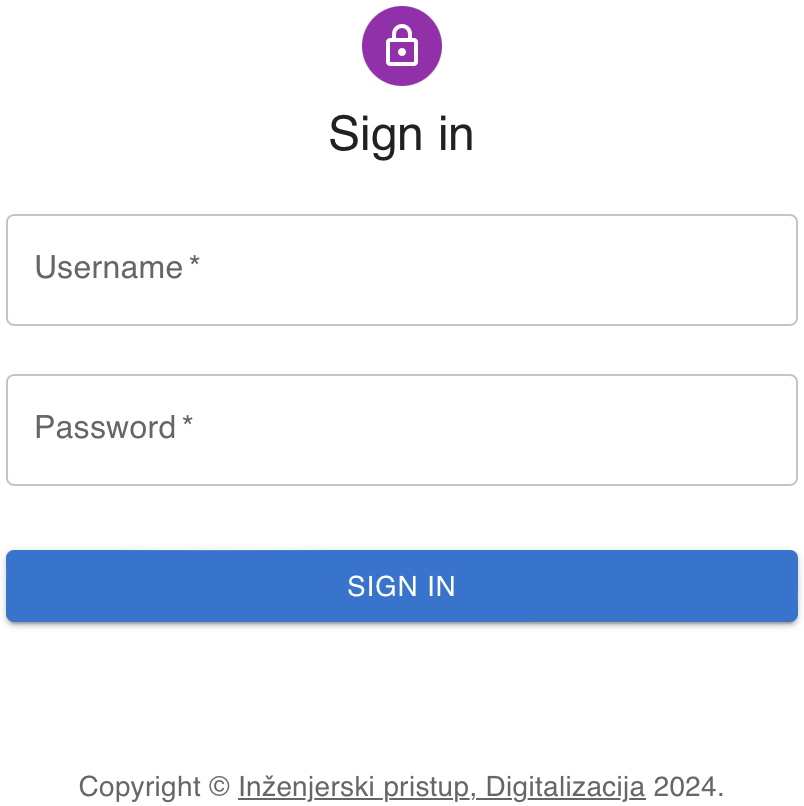
\includegraphics[width=\textwidth]{slike/slika_prijave.png}
			\caption{Slika prijave korisnika u sustav}
			\label{fig:slika_prijave}
		\end{figure}

		\section{Tehnički aspekti i razvojni ciklus}

		Aplikacija  će biti razvijena korištenjem modernih tehnologija kako bi osigurala visoku razinu sigurnosti i performansi. Backend će biti implementiran pomoću popularnog okvira kao što je Django, osiguravajući robusnost i skalabilnost sustava. Kako bi se postigla brza i responzivna korisnička sučelja, frontend će se temeljiti na Reactu.
		Važan aspekt svake aplikacije je korisničko sučelje koje smo dizajnirali tako da je vrlo intuitivno i jednostavno za korištenje. 
		Dizajnerske odluke temelje se na najboljim praksama kako bi se različitim korisnicima osiguralo ugodno iskustvo.
		Kroz pažljivo planiranje korisničkih tokova i jasnu navigaciju, aplikacija će omogućiti korisnicima brz i učinkovit pristup funkcionalnostima.
		Razvoj će se odvijati u iteracijama koristeći agilne metodologije, što će omogućiti fleksibilnost u prilagodbi promjenama zahtjeva. Redovito testiranje, uključujući testiranje jedinica, integracije i sustava, bit će ključno za osiguravanje stabilnosti i performansi aplikacije.
		
		\section{Prava određenih korisnika}
		
		Prijavom u sustav korisniku se dodjeljuju njegova prava. Svaki korisnik ima osnovne mogućnosti:
		\begin{packed_item}
			\item mijenjanje lozinke korisničkog računa
			\item skeniranje dokumenata
			\item pristup povijesti vlastitih skeniranih dokumenata
			\item Nakon skeniranja dokumenta ima pravo potvrditi njegovu točnost, odnosno odbiti ga.
		\end{packed_item}
		S obzirom na osjetljivost financijskih podataka, sigurnost je ključna komponenta. Pristup određenim funkcionalnostima bit će strogo kontroliran putem sustava ovlasti,
		 osiguravajući da svaki korisnik ima pristup samo onim informacijama i radnjama koje su relevantne za njegovu ulogu.
		\newline
		Dodatna prava koja ovise o njegovu položaju u tvrtki su:
		\begin{packed_item}
			\item \textbf{Zaposlenici:} 
					\begin{packed_item}
						\item Imaju pravo slati svoje skenirane dokumente revizoru.
					\end{packed_item}
			\item \textbf{Revizori:} 
					\begin{packed_item}
						\item Imaju odgovornost za pregled svih pristiglih dokumenata i daljnje usmjeravanje prema računovođama
						\item odbijanje dokumenta ako ne zadovoljava potrebne uvjete 
					\end{packed_item}
			\item \textbf{Računovođe:} 
						\begin{packed_item}
						\item Imaju ključnu ulogu u arhiviranju primljenih dokumenata i dodjeljivanju jedinstvenih brojeva arhivama
						\item slanje dokumenata direktoru na potpis
					\end{packed_item}
			\item \textbf{Direktor:}
						\begin{packed_item} 
							\item Ima najveće ovlasti, potpunu preglednost nad svim dokumentima i statistikama zaposlenika
							\item Pregled povijesti dokumenata i zaposlenika
							\item mogućnost dijeljenja odabranih dokumenata na društvene mreže
							\item Jedini ima mogućnost registriranja novih korisnika, pri čemu on i dodjeljuje ulogu svakom novom korisniku. 
							\item Može i obrisati korisnika koji se nalazi u sustavu iz sustava.
						\end{packed_item}
		\end{packed_item}
		
		\section{Slična rješenja}
		
		Ova aplikacija nije jedina takva na tržištu, slična rješenja uključuju Adobe Acrobat za OCR i upravljanje dokumentima, te ABBYY FineReader za napredno optičko prepoznavanje znakova. No ova aplikacija se razlikuje po svojoj kombinaciji funkcionalnosti. Ona će kombinirati najbolje aspekte ovih rješenja i dodati posebne značajke prilagođene potrebama računovodstva. To uključuje automatsku detekciju i organizaciju dokumenata te više razine pristupa.

		\section{Partnerstva i integracije}

		Staviti ćemo naglasak na uspostavu suradnje s drugim tehnološkim tvrtkama i pružateljima usluga kako bi se proširile funkcionalnosti aplikacije. Partnerstva mogu omogućiti pristup dodatnim resursima, stručnost u specifičnim područjima te ubrzanje inovacija.
		Prvenstveno ćemo se fokusirati na partnere koji se bave područjima naprednog OCR-a, sigurnosnih rješenja ili prilagođenih integracija. Kroz partnerstva i integracije, aplikacija će pružiti dodatnu vrijednost korisnicima. Na primjer, mogućnost sinkronizacije podataka s računovodstvenim softverom ili automatsko prepoznavanje i integraciju informacija iz drugih aplikacija može značajno poboljšati korisničko iskustvo.				 Razvojni tim će redovito pratiti tehničke trendove i inovacije kako bi osigurao da partnerstva i integracije prate najnovije tehnološke standarde. Ova proaktivna pristup osigurat će dugoročnu relevantnost aplikacije u dinamičnom okruženju tehnoloških promjena.
		
		\section{Zaključak}
		
		U konačnici, ovim projektom  stvaraju se temelji za razvoj napredne i inovativne web aplikacije koja će uvelike ubrzati i
		poboljšati proces digitalizacije u računovodstvenim tvrtkama i donijeti korisnicima novo i učinkovito rješenje s
		minimaliziranom količinom pogrešaka za obradu dokumenata. Uz kombinaciju tehnoloških rješenja, sigurnosnih mjera i korisničkih sučelja, očekuje se da će ova aplikacija postati ključni alat u optimizaciji poslovnih operacija. 
		Njezina prilagodljivost i skalabilnost čine je perspektivnim rješenjem koje će unaprijediti digitalizaciju dokumenata na novu razinu.
		Kroz ove aktivnosti, projekt će izgraditi snažnu mrežu podrške i suradnje, čime će osigurati da aplikacija ostane fleksibilna i prilagodljiva promjenama u tehnologiji i zahtjevima korisnika.
		\eject
		
		\section{Primjeri u \LaTeX u}
		
		\text{Ovo potpoglavlje izbrisati.}\\

		U nastavku se nalaze različiti primjeri kako koristiti osnovne funkcionalnosti \LaTeX a koje su potrebne za izradu dokumentacije. Za dodatnu pomoć obratiti se asistentu na projektu ili potražiti upute na sljedećim web sjedištima:
		\begin{itemize}
			\item Upute za izradu diplomskog rada u \LaTeX u - \url{https://www.fer.unizg.hr/_download/repository/LaTeX-upute.pdf}
			\item \LaTeX\ projekt - \url{https://www.latex-project.org/help/}
			\item StackExchange za Tex - \url{https://tex.stackexchange.com/}\\
		
		\end{itemize} 	


		
		\noindent \underbar{podcrtani tekst}, \textbf{podebljani tekst}, 	\textit{nagnuti tekst}\\
		\noindent \normalsize primjer \large primjer \Large primjer \LARGE {primjer} \huge {primjer} \Huge primjer \normalsize
				
		\begin{packed_item}
			
			\item  primjer
			\item  primjer
			\item  primjer
			\item[] \begin{packed_enum}
				\item primjer
				\item[] \begin{packed_enum}
					\item[1.a] primjer
					\item[b] primjer
				\end{packed_enum}
				\item primjer
			\end{packed_enum}
			
		\end{packed_item}
		
		\noindent primjer url-a: \url{https://www.fer.unizg.hr/predmet/proinz/projekt}
		
		\noindent posebni znakovi: \# \$ \% \& \{ \} \_ 
		$|$ $<$ $>$ 
		\^{} 
		\~{} 
		$\backslash$ 
		
		
		\begin{longtblr}[
			label=none,
			entry=none
			]{
				width = \textwidth,
				colspec={|X[8,l]|X[8, l]|X[16, l]|}, 
				rowhead = 1,
			} %definicija širine tablice, širine stupaca, poravnanje i broja redaka naslova tablice
			\hline \SetCell[c=3]{c}{\textbf{naslov unutar tablice}}	 \\ \hline[3pt]
			\SetCell{LightGreen}IDKorisnik & INT	&  	Lorem ipsum dolor sit amet, consectetur adipiscing elit, sed do eiusmod  	\\ \hline
			korisnickoIme	& VARCHAR &   	\\ \hline 
			email & VARCHAR &   \\ \hline 
			ime & VARCHAR	&  		\\ \hline 
			\SetCell{LightBlue} primjer	& VARCHAR &   	\\ \hline 
		\end{longtblr}
		

		\begin{longtblr}[
				caption = {Naslov s referencom izvan tablice},
				entry = {Short Caption},
			]{
				width = \textwidth, 
				colspec = {|X[8,l]|X[8,l]|X[16,l]|}, 
				rowhead = 1,
			}
			\hline
			\SetCell{LightGreen}IDKorisnik & INT	&  	Lorem ipsum dolor sit amet, consectetur adipiscing elit, sed do eiusmod  	\\ \hline
			korisnickoIme	& VARCHAR &   	\\ \hline 
			email & VARCHAR &   \\ \hline 
			ime & VARCHAR	&  		\\ \hline 
			\SetCell{LightBlue} primjer	& VARCHAR &   	\\ \hline 
		\end{longtblr}
	


		
		
		%unos slike
		\begin{figure}[H]
			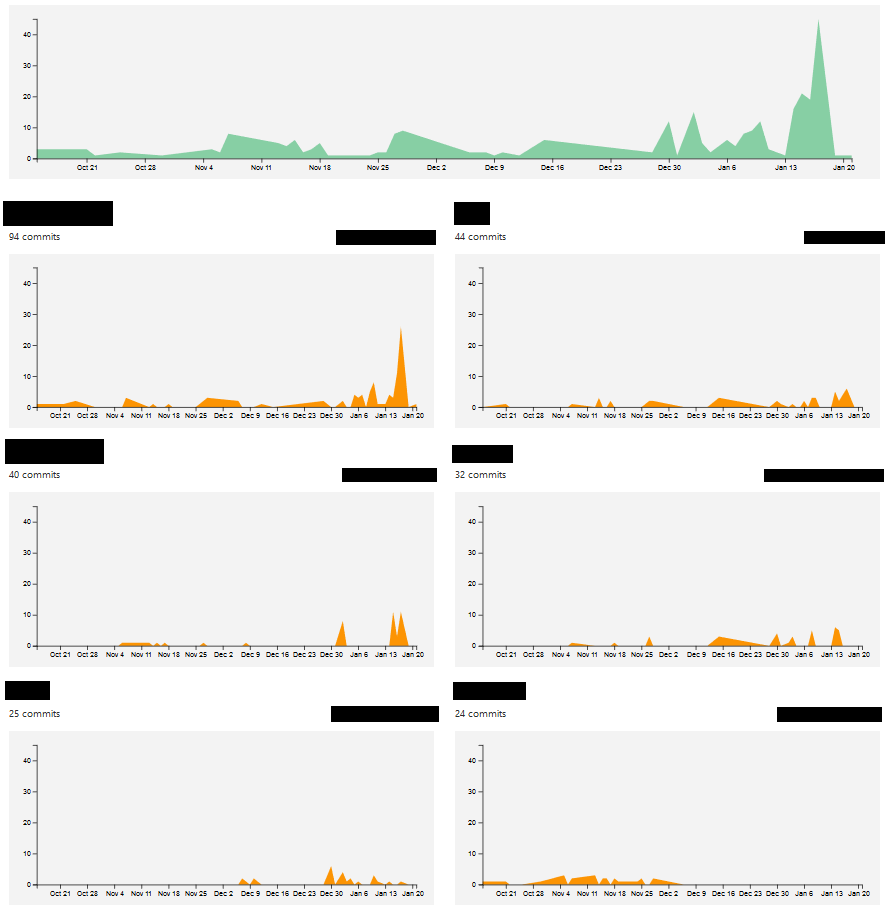
\includegraphics[scale=0.4]{slike/aktivnost.PNG} %veličina slike u odnosu na originalnu datoteku i pozicija slike
			\centering
			\caption{Primjer slike s potpisom}
			\label{fig:promjene}
		\end{figure}
		
		\begin{figure}[H]
			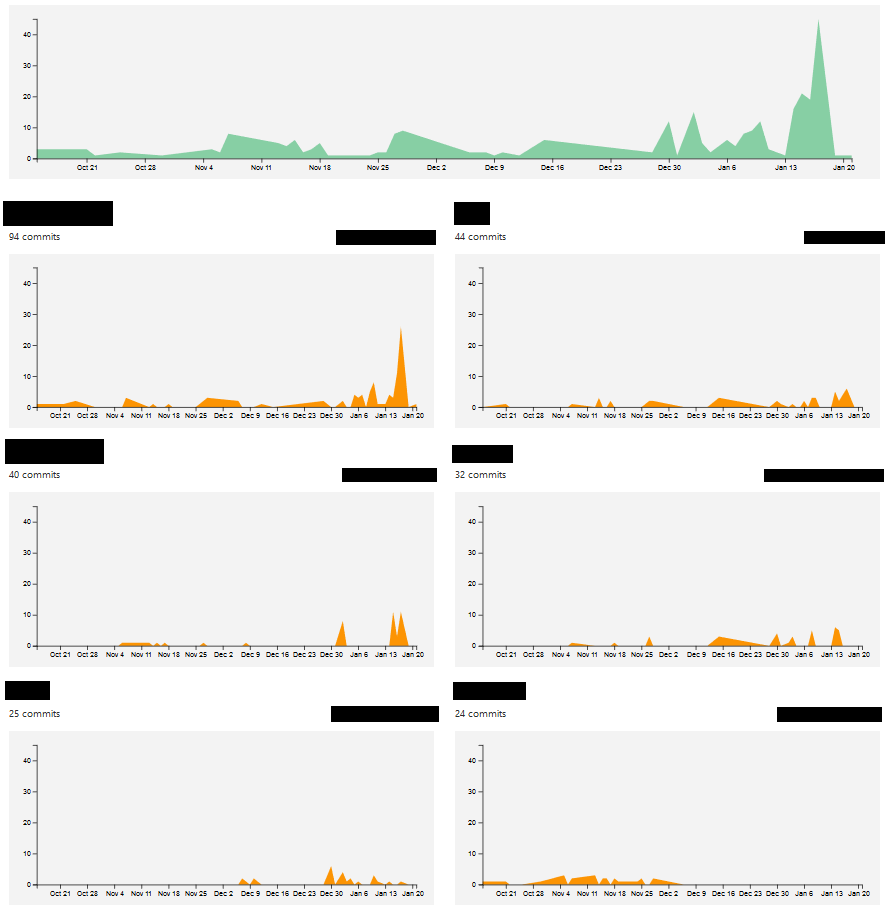
\includegraphics[width=\textwidth]{slike/aktivnost.PNG} %veličina u odnosu na širinu linije
			\caption{Primjer slike s potpisom 2}
			\label{fig:promjene2} %label mora biti drugaciji za svaku sliku
		\end{figure}
		
		Referenciranje slike \ref{fig:promjene2} u tekstu.
		
		\eject
		
	
	\chapter{Specifikacija programske potpore}
		
	\section{Funkcionalni zahtjevi}
			
			\textbf{\textit{dio 1. revizije}}\\
			
			\textit{Navesti \textbf{dionike} koji imaju \textbf{interes u ovom sustavu} ili  \textbf{su nositelji odgovornosti}. To su prije svega korisnici, ali i administratori sustava, naručitelji, razvojni tim.}\\
				
			\textit{Navesti \textbf{aktore} koji izravno \textbf{koriste} ili \textbf{komuniciraju sa sustavom}. Oni mogu imati inicijatorsku ulogu, tj. započinju određene procese u sustavu ili samo sudioničku ulogu, tj. obavljaju određeni posao. Za svakog aktora navesti funkcionalne zahtjeve koji se na njega odnose.}\\
			
			
			\noindent \textbf{Dionici:}
			
			\begin{packed_enum}
				
				\item Zaposlenik
				\item Revizor
				\item Računovođa
				\item Direktor
				\item Razvojni tim
				
			\end{packed_enum}
			

			\noindent \textbf{Aktori i njihovi funkcionalni zahtjevi:}
			
			\begin{packed_enum}
				\item  \underbar{Svaki neregistrirani/neprijavljeni korisnik (inicijator) može:}

				\begin{packed_enum}
					
					\item prijaviti se u sustav
					
				\end{packed_enum}
			
				\item  \underbar{Svaki registrirani/prijavljeni korisnik (inicijator) može:}
				
				\begin{packed_enum}
					
					\item promijeniti lozinku korisničkog računa
					\item vidjeti povijest svojih skeniranja dokumenata
					\item skenirati novi dokument i:

						\begin{packed_enum}
							
							\item potvrditi točnost skeniranog dokumenta
							\item odbiti skenirani dokument

						\end{packed_enum}

				\end{packed_enum}

				\item  \underbar{Zaposlenik (inicijator) može:}
				
				\begin{packed_enum}
					
					\item poslati skenirani dokument revizoru
					
				\end{packed_enum}

				\item  \underbar{Revizor (inicijator) može:}
				
				\begin{packed_enum}
					
					\item provjeriti pristigle dokumente, uključujući svoje, i:

						\begin{packed_enum}
							
							\item potvrditi dokument i proslijediti ga nadležnom računovođi
							\item odbiti dokument

						\end{packed_enum}
					
				\end{packed_enum}

				\item  \underbar{Računovođa (inicijator) može:}

				\begin{packed_enum}
					
					\item arhivirati pristigle dokumente
					\item proslijediti pristigli dokument direktoru na potpis
					
				\end{packed_enum}

				\item  \underbar{Direktor (inicijator) može:}

				\begin{packed_enum}
					
					\item potpisati dokumente pristigle iz računovodstva
					\item vidjeti povijest svih dokumenata
					\item vidjeti povijest i statistike svih zaposlenika
					\item objaviti određeni dokument na društvene mreže 
					\item registrirati novog korisnika i dodijeliti mu ulogu
					\item obrisati postojećeg korisnika
					
				\end{packed_enum}

				\item  \underbar{Baza podataka (sudionik):}

				\begin{packed_enum}

					\item pohranjuje sve podatke o korisnicima i njihovim ovlastima
					\item pohranjuje sve podatke o skeniranim dokumentima
					
				\end{packed_enum}			

			\end{packed_enum}
	
			\eject{}
			
			\subsection{Obrasci uporabe}
				
				\subsubsection{}

					\noindent \underbar{\textbf{UC1 — Prijava u sustav}}
					\begin{packed_item}
	
						\item \textbf{Glavni sudionik:} Bilo koji korisnik
						\item  \textbf{Cilj:} Dobiti pristup korisničkom sučelju
						\item  \textbf{Sudionici:} Baza podataka
						\item  \textbf{Preduvjet:} Posjedovanje vlastitog korisničkog računa
						\item  \textbf{Opis osnovnog tijeka:}
						
						\item[] \begin{packed_enum}
	
							\item Korisnik unosi korisničko ime i lozinku
							\item Baza podataka provjerava ispravnost unesenih podataka
							\item Korisnik dobiva pristup korisničkom sučelju

						\end{packed_enum}
						
						\item  \textbf{Opis mogućih odstupanja:}
						
						\item[] \begin{packed_item}
	
							\item[2.a] Korisnik je unio neispravno korisničko ime ili lozinku
							\item[] \begin{packed_enum}
								
								\item Sustav obavještava korisnika o neuspjeloj prijavi i vraća ga na stranicu za prijavu
								
							\end{packed_enum}
							
						\end{packed_item}

					\end{packed_item}


					\noindent \underbar{\textbf{UC2 — Promjena lozinke korisničkog računa}}
					\begin{packed_item}
	
						\item \textbf{Glavni sudionik:} Bilo koji korisnik
						\item  \textbf{Cilj:} Promijeniti lozinku korisničkog računa
						\item  \textbf{Sudionici:} Baza podataka
						\item  \textbf{Preduvjet:} Korisnik je prijavljen u sustav
						\item  \textbf{Opis osnovnog tijeka:}
						
						\item[] \begin{packed_enum}
	
							\item Korisnik odabire opciju promjene lozinke računa
							\item Korisnik unosi trenutnu lozinku računa
							\item Baza podataka provjerava ispravnost unesene lozinke
							\item Korisnik unosi novu lozinku računa
							\item Baza podataka pohranjuje promjenu lozinke

						\end{packed_enum}
						
						\item  \textbf{Opis mogućih odstupanja:}
						
						\item[] \begin{packed_item}
	
							\item[3.a] Korisnik je unio neispravnu trenutnu	lozinku
							\item[] \begin{packed_enum}
								
								\item Sustav obavještava korisnika o pogrešnom unosu trenutne lozinke i vraća ga na stranicu za unos lozinke
								
							\end{packed_enum}
							
						\end{packed_item}

					\end{packed_item}


					\noindent \underbar{\textbf{UC3 — Pregled povijesti skeniranih dokumenata}}
					\begin{packed_item}
	
						\item \textbf{Glavni sudionik:} Bilo koji korisnik
						\item  \textbf{Cilj:} Vidjeti povijest svojih skeniranih dokumenata
						\item  \textbf{Sudionici:} Baza podataka
						\item  \textbf{Preduvjet:} Korisnik je prijavljen u sustav
						\item  \textbf{Opis osnovnog tijeka:}
						
						\item[] \begin{packed_enum}
	
							\item Aplikacija korisniku na početnom zaslonu prikazuje njegovu povijest skeniranih dokumenata

						\end{packed_enum}

					\end{packed_item}


					\noindent \underbar{\textbf{UC4 — Skeniranje novog dokumenta}}
					\begin{packed_item}
	
						\item \textbf{Glavni sudionik:} Bilo koji korisnik
						\item  \textbf{Cilj:} Skenirati novi dokument
						\item  \textbf{Sudionici:} Baza podataka
						\item  \textbf{Preduvjet:} Korisnik je prijavljen u sustav
						\item  \textbf{Opis osnovnog tijeka:}
						
						\item[] \begin{packed_enum}
	
							\item Korisnik na početnom zaslonu odabire opciju za skeniranje novog dokumenta
							\item Korisnik učitava dokument u obliku slike u aplikaciju
							\item Aplikacija provjerava ispravnost učitanog dokumenta
							\item Aplikacija korisniku prikazuje učitani dokument i razvsrtava ga u jednu od kategorija:

								\begin{packed_enum}
									
									\item račun
									\item ponuda
									\item interni dokument

								\end{packed_enum}

							\item Korisnik potvrđuje točnost učitanog dokumenta ili ga odbija

						\end{packed_enum}

						\item  \textbf{Opis mogućih odstupanja:}
						
						\item[] \begin{packed_item}
	
							\item[3.a] Dokument nije ispravno skeniran
							\item[] \begin{packed_enum}
								
								\item Aplikacija obavještava korisnika o neuspjelom skeniranju i vraća ga na zaslon za učitavanje dokumenta
								
							\end{packed_enum}
							
						\end{packed_item}

					\end{packed_item}


					\noindent \underbar{\textbf{UC5 — Slanje skeniranog dokumenta revizoru}}
					\begin{packed_item}
	
						\item \textbf{Glavni sudionik:} Zaposlenik
						\item  \textbf{Cilj:} Poslati skenirani dokument revizoru
						\item  \textbf{Sudionici:} Baza podataka, revizor
						\item  \textbf{Preduvjet:} Zaposlenik se prijavio u sustav skenirao je dokument
						\item  \textbf{Opis osnovnog tijeka:}
						
						\item[] \begin{packed_enum}
	
							\item Zaposlenik odabire opciju za slanje skeniranog dokumenta revizoru
							\item Aplikacija prikazuje popis svih revizora
							\item Zaposlenik odabire revizora kojemu želi poslati dokument
							\item Aplikacija šalje dokument odabranom revizoru

						\end{packed_enum}

					\end{packed_item}


					\noindent \underbar{\textbf{UC6 — Provjera pristiglih dokumenata}}
					\begin{packed_item}
	
						\item \textbf{Glavni sudionik:} Revizor
						\item  \textbf{Cilj:} Provjeriti pristigle dokumente, uključujući svoje
						\item  \textbf{Sudionici:} Baza podataka, zaposlenik, računovođa
						\item  \textbf{Preduvjet:} Revizor je prijavljen u sustav i ima pristiglih dokumenata
						\item  \textbf{Opis osnovnog tijeka:}
						
						\item[] \begin{packed_enum}
	
							\item Revizor odabire opciju za provjeru pristiglog dokumenta
							\item Aplikacija revizoru prikazuje dokument
							\item Revizor potvrđuje točnost dokumenta ili ga odbija:
							
							\begin{packed_enum}
								
								\item točan dokument aplikacija proslijeđuje nadležnom računovođi
								\item netočan dokument aplikacija odbacuje i o tome dojavljuje zaposlenika

							\end{packed_enum}

						\end{packed_enum}

					\end{packed_item}


					\noindent \underbar{\textbf{UC7 — Arhiviranje pristiglih dokumenata}}
					\begin{packed_item}
	
						\item \textbf{Glavni sudionik:} Računovođa
						\item  \textbf{Cilj:} Arhivirati pristigle dokumente
						\item  \textbf{Sudionici:} Baza podataka
						\item  \textbf{Preduvjet:} Računovođa je prijavljen u sustav i ima pristiglih dokumenata
						\item  \textbf{Opis osnovnog tijeka:}
						
						\item[] \begin{packed_enum}
	
							\item Računovođa odabire opciju za arhiviranje pristiglog dokumenta
							\item Aplikacija dojavljuje bazi podataka da arhivira dokument
							\item Baza podataka arhivira dokument i dodjeljuje mu jedinstveni broj arhiva

						\end{packed_enum}

					\end{packed_item}


					\noindent \underbar{\textbf{UC8 — Slanje dokumenata na potpis direktoru}}
					\begin{packed_item}
	
						\item \textbf{Glavni sudionik:} Računovođa
						\item  \textbf{Cilj:} Poslati dokument direktoru na potpis
						\item  \textbf{Sudionici:} Direktor
						\item  \textbf{Preduvjet:} Računovođa je prijavljen u sustav i ima pristiglih dokumenata
						\item  \textbf{Opis osnovnog tijeka:}
						
						\item[] \begin{packed_enum}
	
							\item Računovođa odabire opciju za slanje dokumenta direktoru na potpis
							\item Aplikacija šalje dokument direktoru na potpis
							\item Direktor dobiva obavijest o pristiglom dokumentu

						\end{packed_enum}

					\end{packed_item}


					\noindent \underbar{\textbf{UC9 — Potpisivanje dokumenata}}
					\begin{packed_item}
	
						\item \textbf{Glavni sudionik:} Direktor
						\item  \textbf{Cilj:} Potpisati dokumente pristigle iz računovodstva
						\item  \textbf{Sudionici:} Baza podataka, računovođa
						\item  \textbf{Preduvjet:} Direktor je prijavljen u sustav i ima pristiglih dokumenata
						\item  \textbf{Opis osnovnog tijeka:}
						
						\item[] \begin{packed_enum}
	
							\item Direktor odabire opciju za potpisivanje dokumenta
							\item Aplikacija dojavljuje bazi podataka da je dokument potpisan
							\item Baza podataka označava dokument kao potpisan
							\item Aplikacija šalje potpisani dokument računovođi

						\end{packed_enum}

					\end{packed_item}


					\noindent \underbar{\textbf{UC10 — Pregled povijesti dokumenata}}	
					\begin{packed_item}
	
						\item \textbf{Glavni sudionik:} Direktor
						\item  \textbf{Cilj:} Vidjeti povijest svih dokumenata
						\item  \textbf{Sudionici:} Baza podataka
						\item  \textbf{Preduvjet:} Direktor je prijavljen u sustav
						\item  \textbf{Opis osnovnog tijeka:}
						
						\item[] \begin{packed_enum}
	
							\item Aplikacija direktoru na početnom zaslonu prikazuje povijest svih dokumenata

						\end{packed_enum}

					\end{packed_item}


					\noindent \underbar{\textbf{UC11 — Pregled povijesti i statistika zaposlenika}}
					\begin{packed_item}
	
						\item \textbf{Glavni sudionik:} Direktor
						\item  \textbf{Cilj:} Vidjeti povijest i statistike svih zaposlenika
						\item  \textbf{Sudionici:} Baza podataka
						\item  \textbf{Preduvjet:} Direktor je prijavljen u sustav
						\item  \textbf{Opis osnovnog tijeka:}
						
						\item[] \begin{packed_enum}
	
							\item Aplikacija direktoru na početnom zaslonu prikazuje povijest i statistike svih zaposlenika

						\end{packed_enum}

					\end{packed_item}


					\noindent \underbar{\textbf{UC12 — Registracija novog korisnika}}
					\begin{packed_item}
	
						\item \textbf{Glavni sudionik:} Direktor
						\item  \textbf{Cilj:} Registrirati novog korisnika i dodijeliti mu ulogu
						\item  \textbf{Sudionici:} Baza podataka
						\item  \textbf{Preduvjet:} Direktor je prijavljen u sustav
						\item  \textbf{Opis osnovnog tijeka:}
						
						\item[] \begin{packed_enum}
	
							\item Direktor odabire opciju za registraciju novog korisnika
							\item Aplikacija prikazuje formu za registraciju novog korisnika
							\item Direktor unosi podatke o novom korisniku, uključujući njegovu ulogu
							\item Aplikacija provjerava ispravnost unesenih podataka
							\item Aplikacija dojavljuje bazi podataka da registrira novog korisnika
							\item Baza podataka pohranjuje podatke o novom korisniku

						\end{packed_enum}

						\item  \textbf{Opis mogućih odstupanja:}
						
						\item[] \begin{packed_item}
	
							\item[4.a] Direktor je unio neispravne podatke o novom korisniku
							\item[] \begin{packed_enum}
								
								\item Aplikacija obavještava direktora o neuspjeloj registraciji i vraća ga na formu za registraciju novog korisnika

							\end{packed_enum}
							
						\end{packed_item}

					\end{packed_item}


					\noindent \underbar{\textbf{UC13 - Brisanje postojećeg korisnika}}
					\begin{packed_item}
	
						\item \textbf{Glavni sudionik:} Direktor
						\item  \textbf{Cilj:} Obrisati postojećeg korisnika
						\item  \textbf{Sudionici:} Baza podataka
						\item  \textbf{Preduvjet:} Direktor je prijavljen u sustav i postojeći korisnik je registriran u sustavu
						\item  \textbf{Opis osnovnog tijeka:}
						
						\item[] \begin{packed_enum}
	
							\item Direktor odabire opciju za brisanje postojećeg korisnika
							\item Aplikacija prikazuje popis svih korisnika
							\item Direktor odabire korisnika kojeg želi obrisati
							\item Aplikacija dojavljuje bazi podataka da obriše korisnika
							\item Baza podataka briše korisnika

						\end{packed_enum}

					\end{packed_item}


					\noindent \underbar{\textbf{UC14 - Objavljivanje dokumenta na društvene mreže}}
					\begin{packed_item}
	
						\item \textbf{Glavni sudionik:} Direktor
						\item  \textbf{Cilj:} Objaviti određeni dokument na društvene mreže
						\item  \textbf{Sudionici:} Baza podataka, društvene mreže
						\item  \textbf{Preduvjet:} Direktor je prijavljen u sustav i dokument je potpisan
						\item  \textbf{Opis osnovnog tijeka:}
						
						\item[] \begin{packed_enum}
	
							\item Direktor odabire opciju za objavljivanje dokumenta na društvene mreže
							\item Aplikacija direktoru prikazuje izbor društvenih mreža
							\item Direktor odabire društvenu mrežu na koju želi objaviti dokument
							\item Aplikacija direktora preusmjerava na odabranu društvenu mrežu

						\end{packed_enum}

					\end{packed_item}


					\noindent \underbar{\textbf{UC15 - Odjava iz sustava}}
					\begin{packed_item}
	
						\item \textbf{Glavni sudionik:} Korisnik
						\item  \textbf{Cilj:} Odjaviti se iz sustava
						\item  \textbf{Sudionici:} -
						\item  \textbf{Preduvjet:} Korisnik je prijavljen u sustav
						\item  \textbf{Opis osnovnog tijeka:}
						
						\item[] \begin{packed_enum}
	
							\item Korisnik odabire opciju za odjavu iz sustava
							\item Aplikacija korisnika odjavljuje iz sustava i preusmjerava na stranicu za prijavu

						\end{packed_enum}

					\end{packed_item}

				\eject{}
					
				\subsubsection{Dijagrami obrazaca uporabe}
					
					\textit{Prikazati odnos aktora i obrazaca uporabe odgovarajućim UML dijagramom. Nije nužno nacrtati sve na jednom dijagramu. Modelirati po razinama apstrakcije i skupovima srodnih funkcionalnosti.}

					\begin{figure}[H]
						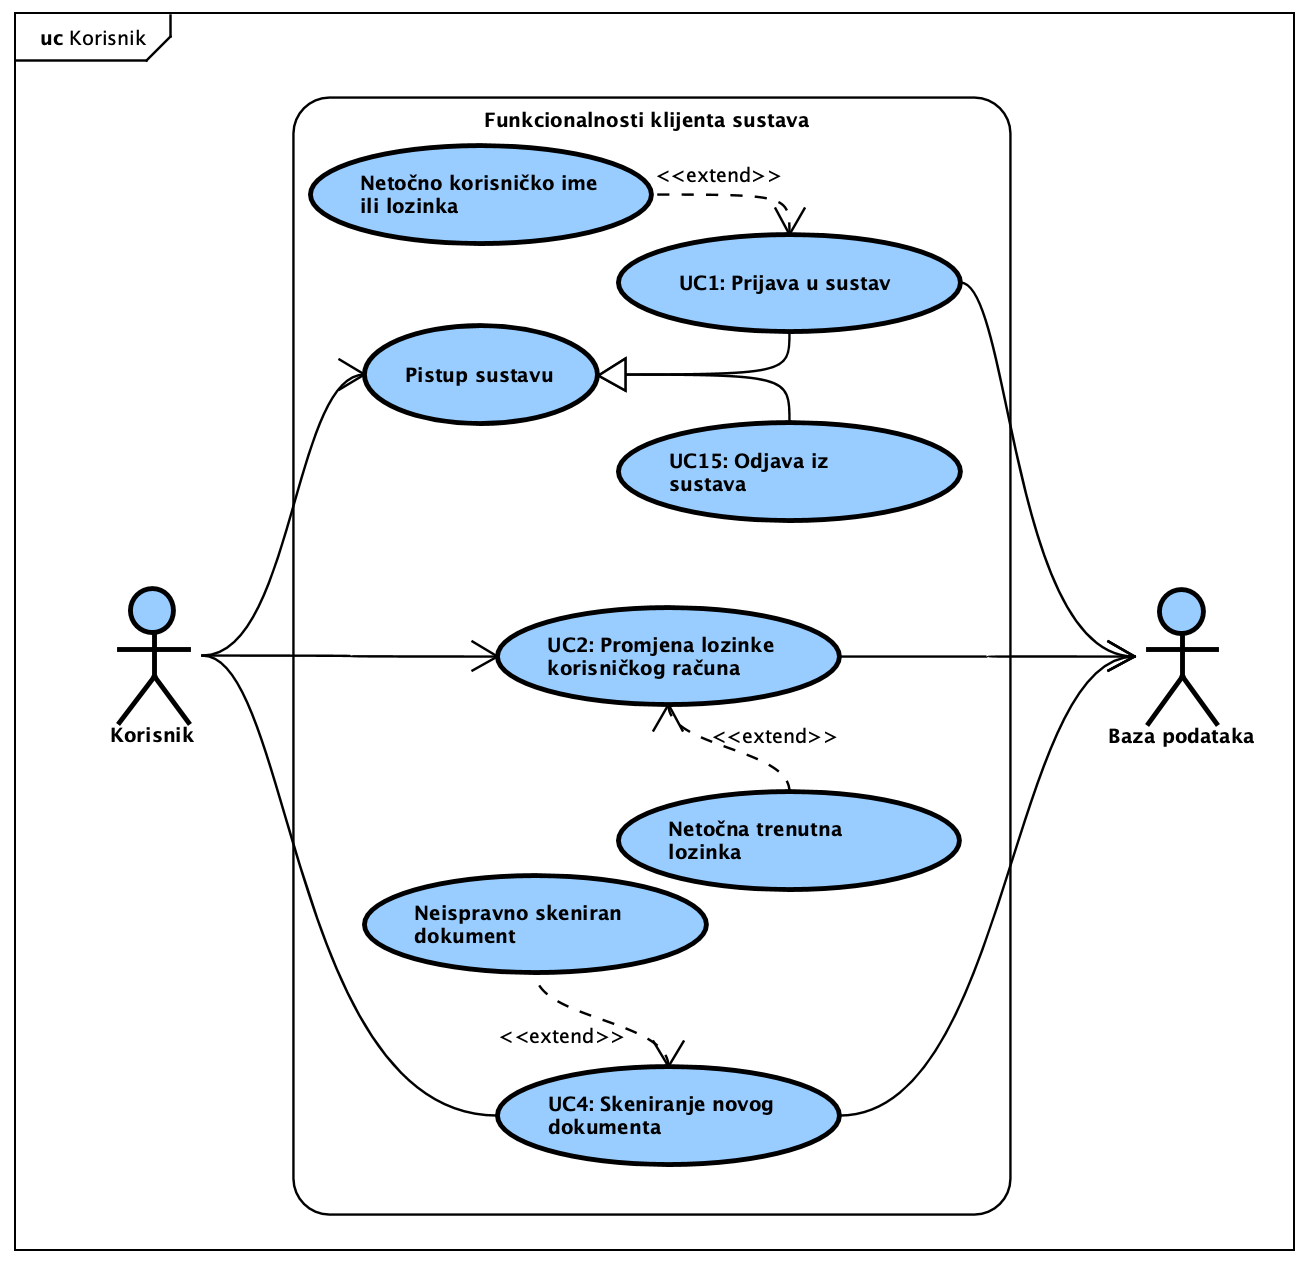
\includegraphics[width=\textwidth]{slike/UseCase_Korisnik.png} %veličina u odnosu na širinu linije
						\caption{Dijagram obrasca uporabe, funkcionalnost korisnika}
						\label{fig:usecase_korisnik} %label mora biti drugaciji za svaku sliku
					\end{figure}

					\begin{figure}[H]
						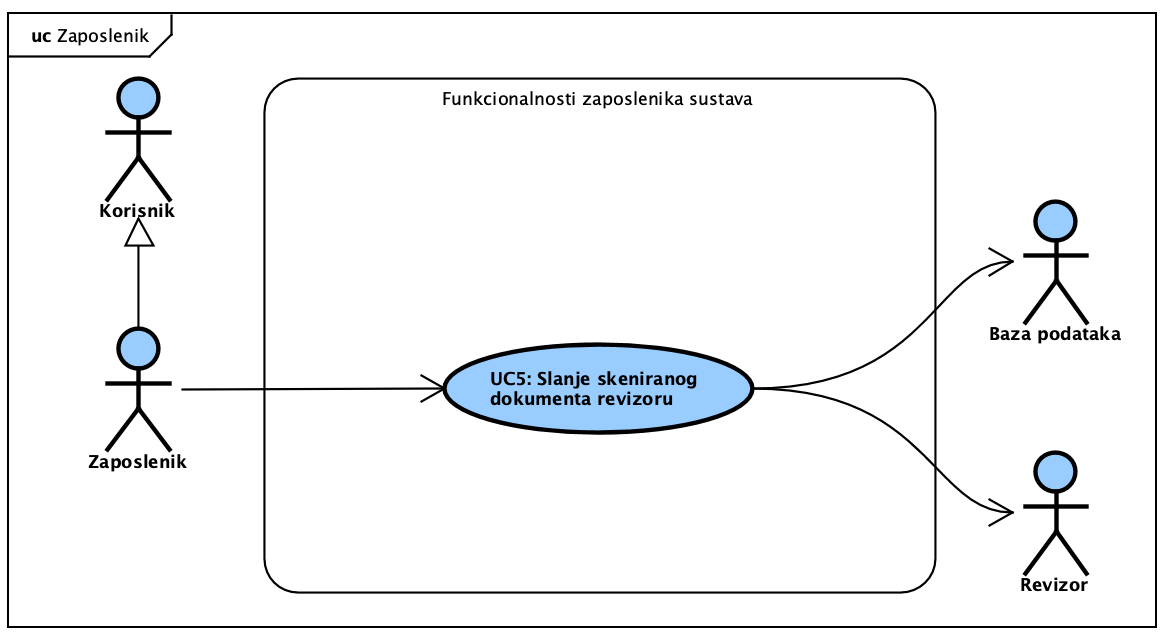
\includegraphics[width=\textwidth]{slike/UseCase_Zaposlenik.png}
						\caption{Dijagram obrasca uporabe, funkcionalnost zaposlenika}
						\label{fig:usecase_zaposlenik}
					\end{figure}

					\begin{figure}[H]
						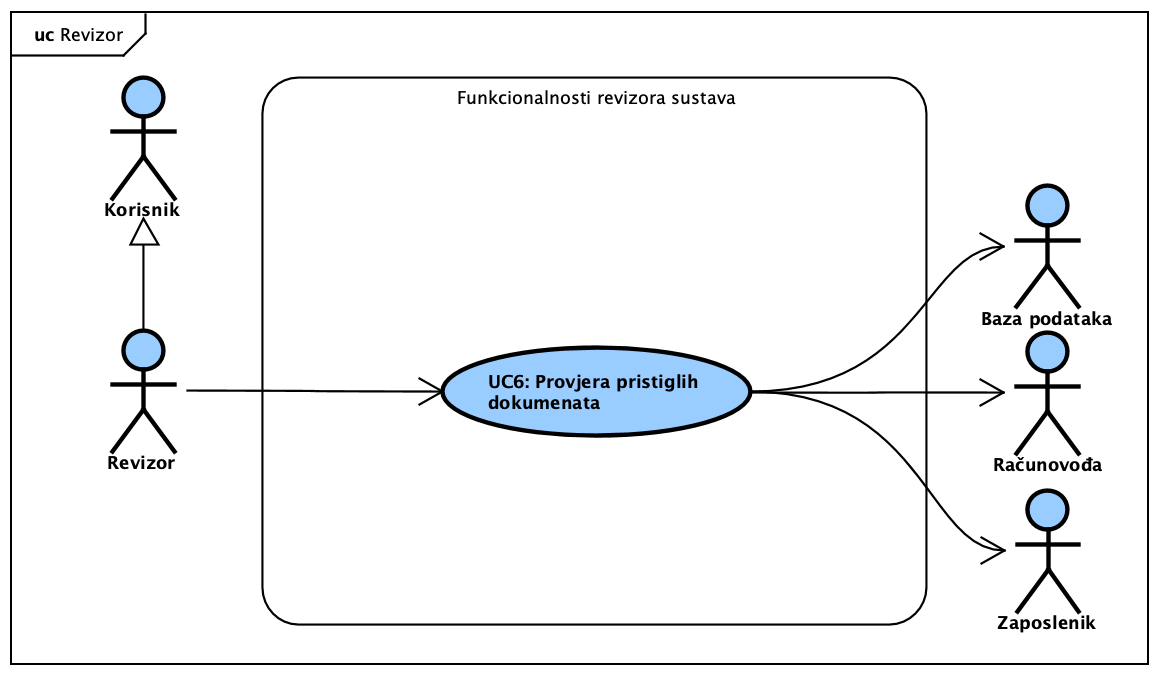
\includegraphics[width=\textwidth]{slike/UseCase_Revizor.png}
						\caption{Dijagram obrasca uporabe, funkcionalnost revizora}
						\label{fig:usecase_revizor}
					\end{figure}

					\begin{figure}[H]
						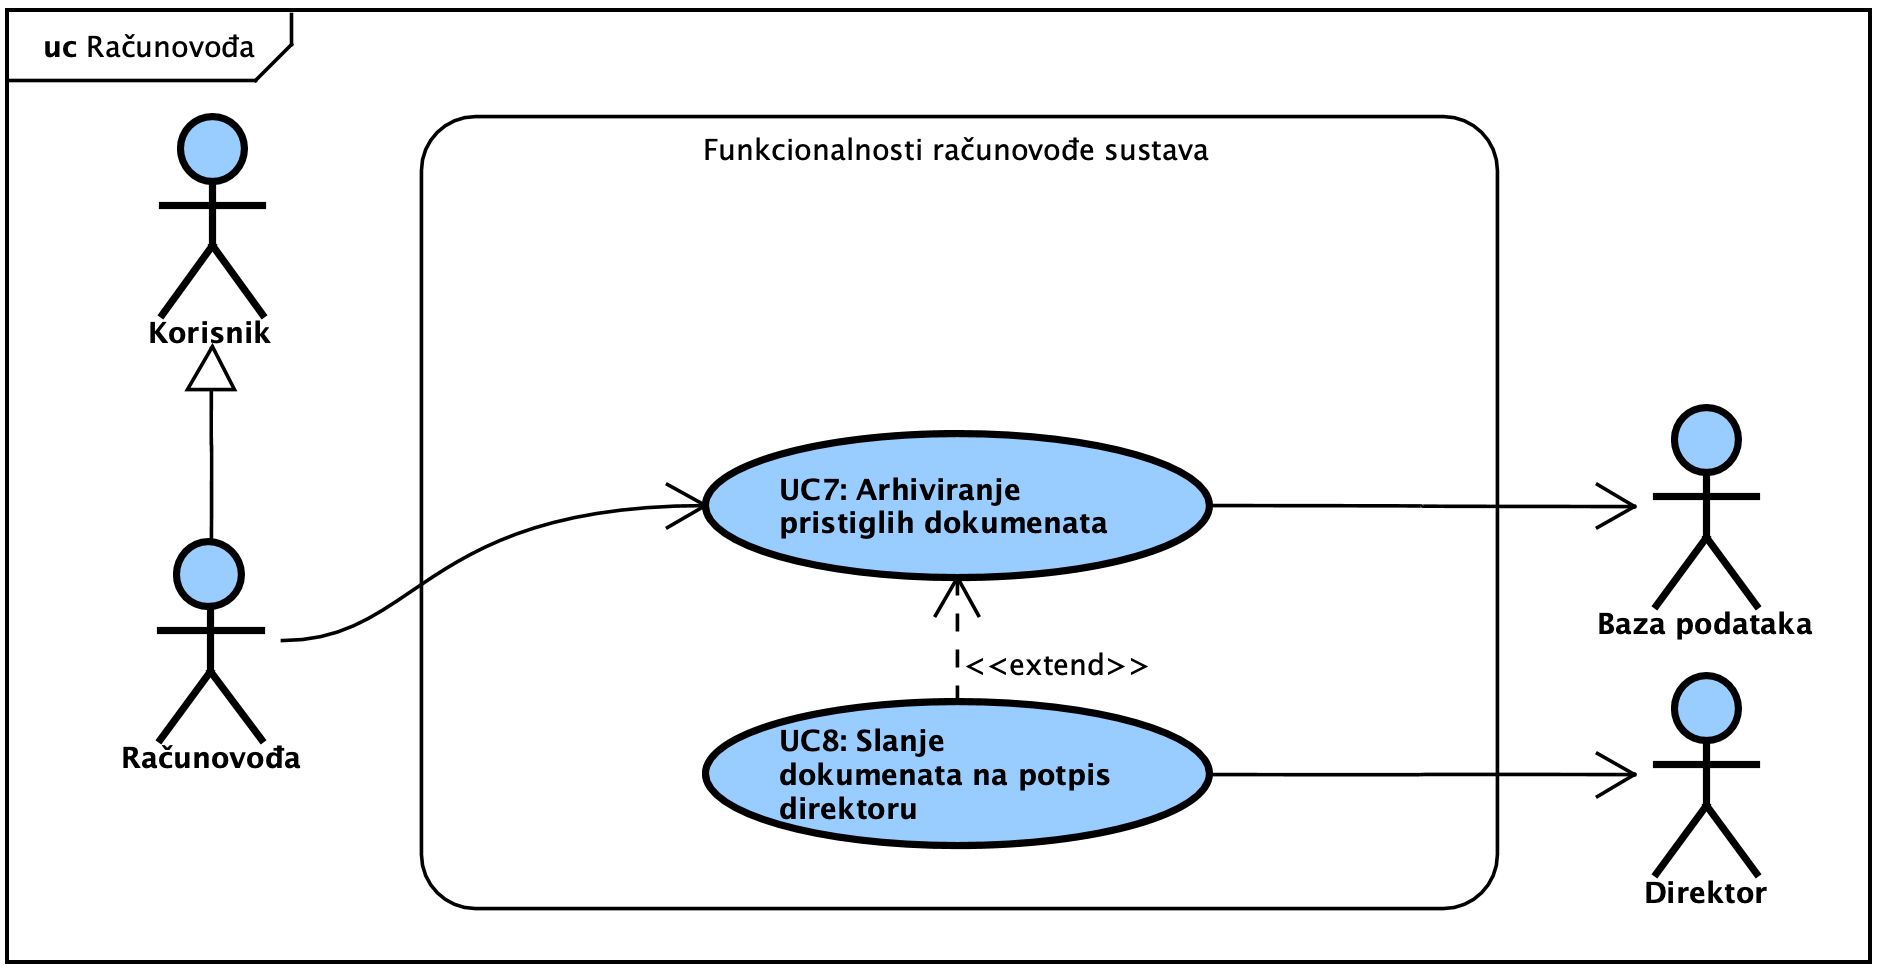
\includegraphics[width=\textwidth]{slike/UseCase_Racunovoda.png}
						\caption{Dijagram obrasca uporabe, funkcionalnost računovođe}
						\label{fig:usecase_racunovoda}
					\end{figure}

					\begin{figure}[H]
						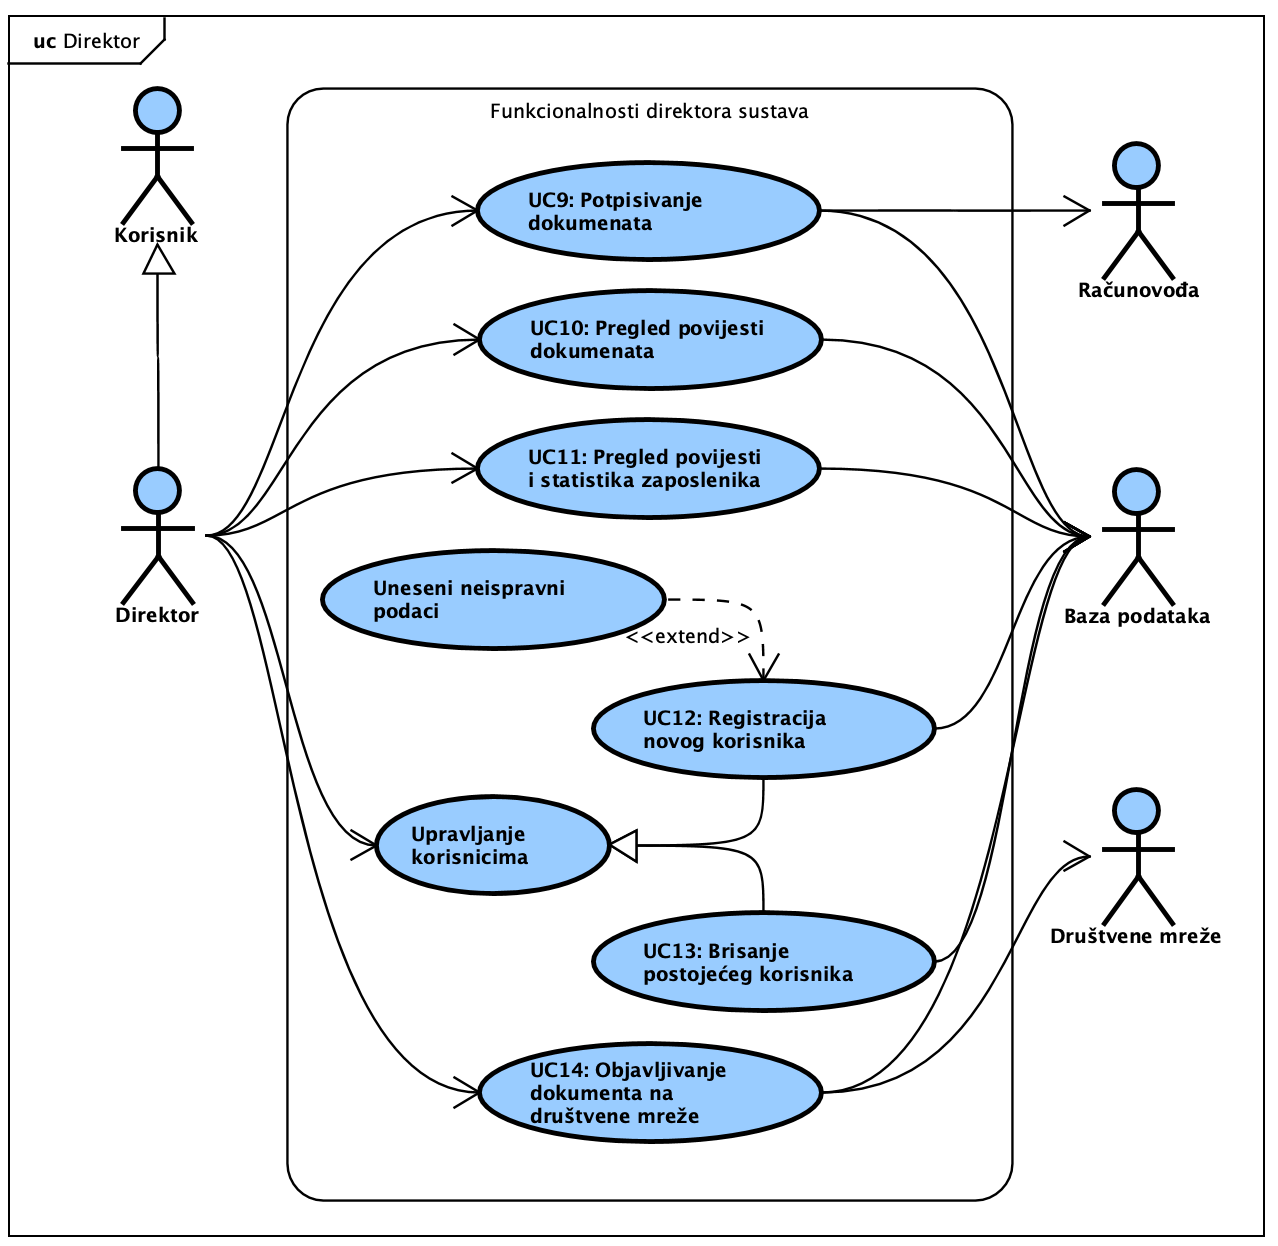
\includegraphics[width=\textwidth]{slike/UseCase_Direktor.png}
						\caption{Dijagram obrasca uporabe, funkcionalnost direktora}
						\label{fig:usecase_direktor}
					\end{figure}
				\eject{}
				
			\subsection{Sekvencijski dijagrami}
				
				\textbf{\textit{dio 1. revizije}}\\
				
				\textit{Nacrtati sekvencijske dijagrame koji modeliraju najvažnije dijelove sustava (max. 4 dijagrama). Ukoliko postoji nedoumica oko odabira, razjasniti s asistentom. Uz svaki dijagram napisati detaljni opis dijagrama.}

				\begin{figure}[H]
						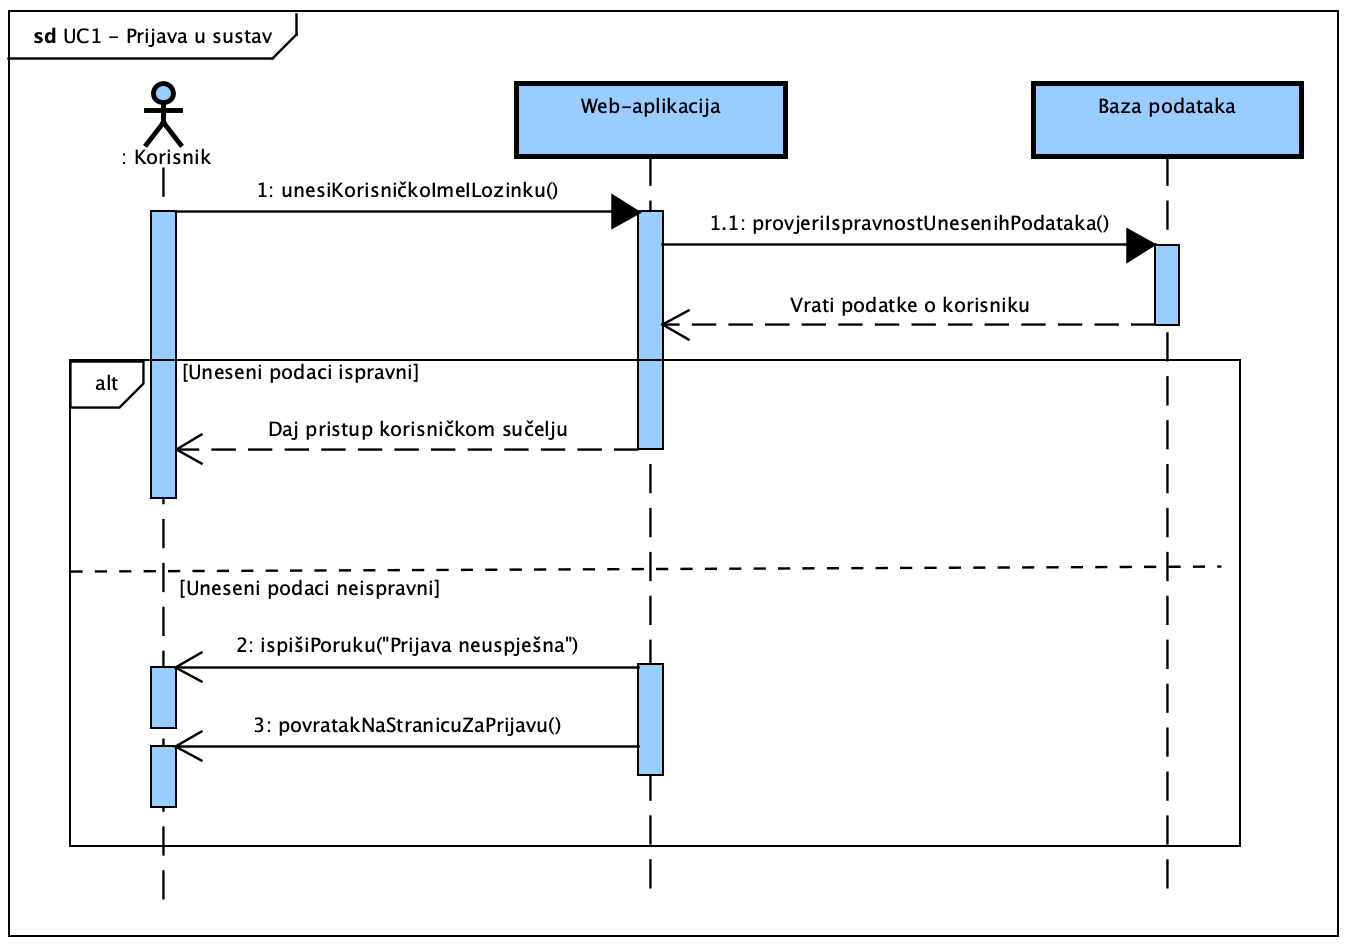
\includegraphics[width=\textwidth]{slike/Sequence_UC01.png}
						\caption{Sekvencijski dijagram za UC01}
						\label{fig:sequence_UC01}
					\end{figure}

					\begin{figure}[H]
						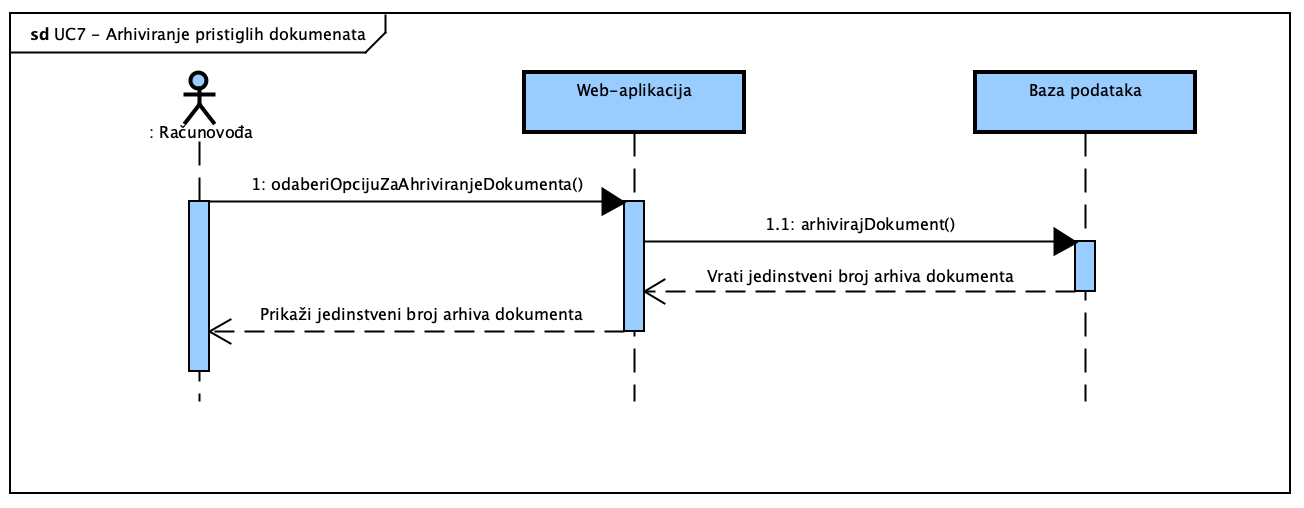
\includegraphics[width=\textwidth]{slike/Sequence_UC07.png}
						\caption{Sekvencijski dijagram za UC07}
						\label{fig:sequence_UC07}
					\end{figure}

					\begin{figure}[H]
						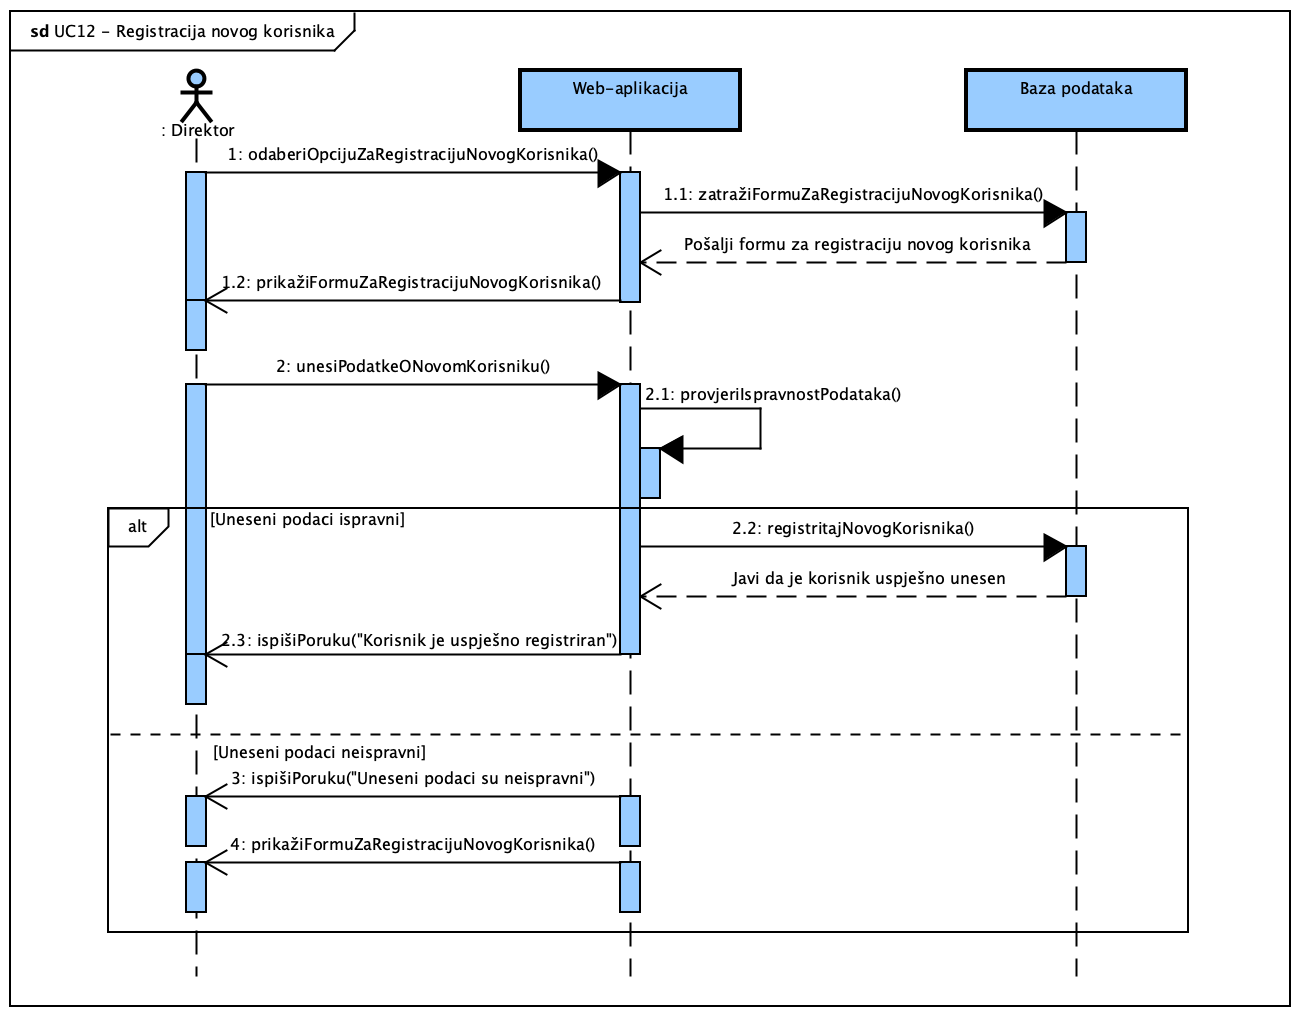
\includegraphics[width=\textwidth]{slike/Sequence_UC12.png}
						\caption{Sekvencijski dijagram za UC12}
						\label{fig:sequence_UC12}
					\end{figure}

					\begin{figure}[H]
						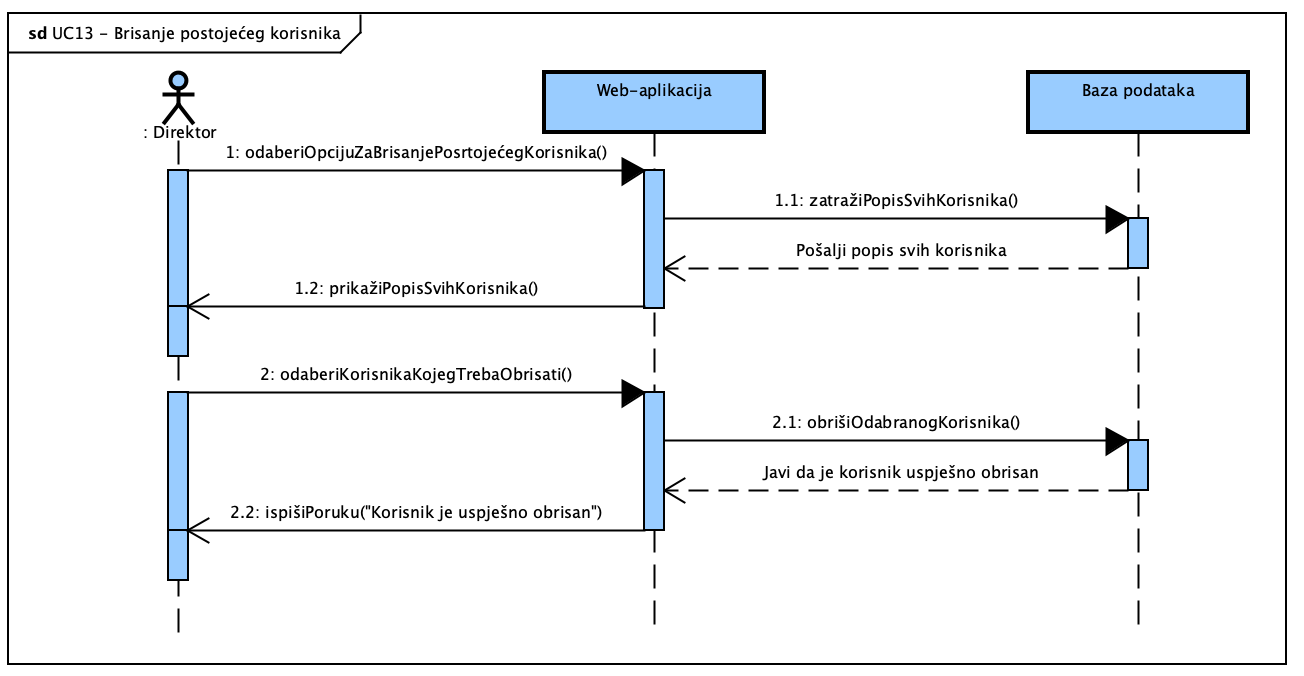
\includegraphics[width=\textwidth]{slike/Sequence_UC13.png}
						\caption{Sekvencijski dijagram za UC13}
						\label{fig:sequence_UC13}
					\end{figure}
			\eject{}
	
		\section{Ostali zahtjevi}
		
			\textbf{\textit{dio 1. revizije}}\\
		 
			\textit{Nefunkcionalni zahtjevi i zahtjevi domene primjene dopunjuju funkcionalne zahtjeve. Oni opisuju \textbf{kako se sustav treba ponašati} i koja \textbf{ograničenja} treba poštivati (performanse, korisničko iskustvo, pouzdanost, standardi kvalitete, sigurnost...). Primjeri takvih zahtjeva u Vašem projektu mogu biti: podržani jezici korisničkog sučelja, vrijeme odziva, najveći mogući podržani broj korisnika, podržane web/mobilne platforme, razina zaštite (protokoli komunikacije, kriptiranje...)... Svaki takav zahtjev potrebno je navesti u jednoj ili dvije rečenice.}
			 
			 
			 
	
	\chapter{Arhitektura i dizajn sustava}
		
		\text{ Arhitektura se može podijeliti na četiri podsustava:}
		\begin{itemize}
			\item 	\text{Web poslužitelj}
			\item 	\text{Web aplikacija}
			\item 	\text{Baza podataka}
			\item 	\text{Domaćin za pohranu slika}
		\end{itemize}

			\begin{figure}[H]
				\includegraphics[scale=0.5]{slike/opis_arhitekture.png} %veličina slike u odnosu na originalnu datoteku i pozicija slike
				\centering
				\caption{Arhitektura sustava}
			\end{figure}
		\textbf{Web preglednik} je alat koji korisniku omogućava pregled web stranica i  svih sadržaja povezanih s isitima. Svaki web preglednik može prevesti kod web aplikacije. Korisnik putem web preglednika šalje zahtjeve na poslužitelj.

		\textbf{Web poslužitelj} ima zadaću vršiti komunikaciju između klijenta i aplikacije. Komunikacija se odvija pomoću HTTP protokola(\textit{Hyper Text Transfer Protocol}). Poslužitelj je ili pokretač web aplikacije, ili server na kojem je web aplikacija postavljena.

		\textbf{Web aplikacija} služi za obradu zahtjeva. Ovisno o zahtjevu, web aplikacija pristupa bazi podataka ili domaćinu za pohranu slika te korisniku vraća generirani HTML dokument koji je vidljiv u web pregledniku.

		Programski jezik koji je korišten za izradu web aplikacije je Pyhton za \textit{backend} i Javascript za \textit{frontend}. Preciznije za \textit{backend} dio koristi se Django, a za \textit{frontend} dio koristi se React. Time smo odvojili \textit{backend} za logiku i obradu podataka, a \textit{frontend} za komunikaciju s korisnikom. Django služi za upravljanje podacima te omogućava definiranje modela podataka i logike aplikacije. React služi za kreiranje korisničkog sučelja. Omogućava brzo i efikasno kreiranje dinamičkih i interaktivnih korisničkih sučelja. Razvojno okruženje u kojem radimo je Microsoft Visual Studio Code.

		\textbf{Domaćin za pohranu slika} je vanjski servis na koji se spremaju slike iz korsničkih zahtjeva poslanih iz web preglednika. Za to koristimo \url{https://imgur.com/}.


				
		\section{Baza podataka}

		Za našu aplikaciju koristit ćemo relacijsku bazu podataka koja će nam olakšati modeliranje samog zadatka. 
		Relacijska baza podataka je baza podataka koja je organizirana u skup tablica koje su međusobno povezane. 
		Svaka tablica predstavlja jednu entitetnu klasu, a svaki redak tablice predstavlja jedan objekt dok stupci predstavljaju atribute. 
		Svaki objekt ima svoj jedinstveni identifikator koji se zove primarni ključ, a može imati i strane ključeve koji su referenca na primarni ključ nekog drugog objekta.
		Baza podataka se koristi za brzu i jednostavnu pohranu podataka koje naknadno možemo lako dohvatiti ili promijeniti.
		Baza podataka naše aplikacije sadrži slijedeće entitete: 

		\begin{packed_item}
			\item  Korisnik
			\item  Pripada
			\item  Grupa
			\item  SpecijalizacijaRačunovođe
			\item  Dokument
			\item  Račun
			\item  Ponuda
			\item  InterniDokument
			\item  NedefiniraniDokument
			\item  Arhiva
			\item  RačunArhiviran
			\item  PonudaArhivirana
			\item  InterniDokumentArhiviran
			\item  NedefiniraniDokumentArhiviran
			\item  Artikl
			\item  NaRačunu
			\item  UPonudi
			\item  NaArhiviranomRačunu
			\item  UArhiviranojPonudi
		\end{packed_item}
		
			\subsection{Opis tablica}
			

				\textbf{Korisnik}: ovaj entitet sadrži sve informacije o korisniku aplikacije. Sadrži atribute: KorisnikId, Ime, Prezime, E-mail, Zaporka, KorisnickoIme, JeAdmin, ZadnjiLogin, JeAktivan, DatumZaposlenja. KorisnikId je primarni ključ.
				Veze s entitetom Korisnik su: One-to-many veza s entitetom Dokument preko atributa KorisnikId,
				One-to-many veza s entitetom Dokument preko atributa KorisnikId (ZaPotvrditiOdDirektoraKorisnikId),
				One-to-many veza s entitetom Dokument preko atributa KorisnikId (ZaPotvrditiOdRevizoraKorisnikId),
				One-to-many veza s entitetom Dokument preko atributa KorisnikId (ZaPotvrditiOdRačunovođeKorisnikId),
				One-to-many veza s entitetom Arhiva preko atributa KorisnikId,
				One-to-many veza s entitetom Arhiva preko atributa KorisnikId (PotvrdioRevizorKorisnikId),
				One-to-many veza s entitetom Arhiva preko atributa KorisnikId (PotvrdioRačunovođaKorisnikId),
				One-to-many veza s entitetom Arhiva preko atributa KorisnikId (PotvrdioDirektorKorisnikId),
				One-to-many veza s entitetom Pripada preko atributa KorisnikId,
				One-to-many veza s entitetom SpecijalizacijaRačunovođe preko atributa KorisnikId.\\
				
				
				\begin{longtblr}[
					label=none,
					entry=none
					]{
						width = \textwidth,
						colspec={|X[8,l]|X[6, l]|X[20, l]|}, 
						rowhead = 1,
					} %definicija širine tablice, širine stupaca, poravnanje i broja redaka naslova tablice
					\hline \SetCell[c=3]{c}{\textbf{Korisnik}}	 \\ \hline[3pt]
					\SetCell{LightGreen}KorisnikId & INT	&  	jedinstveni identifikator korisnika  	\\ \hline
					Ime	& VARCHAR &   ime korisnika	\\ \hline 
					Prezime & VARCHAR &  prezime korisnika \\ \hline 
					E-mail & VARCHAR	&  	E-mail korisnika	\\ \hline 
					Zaporka	& VARCHAR &   hash zaporke	\\ \hline 
					KorisnickoIme	& VARCHAR &   korisničko ime korisnika	\\ \hline 
					JeAdmin	& BOOLEAN &   oznaka je li korisnik admin aplikacije	\\ \hline 
					ZadnjiLogin	& DATETIME &   datum i vrijeme zadnjeg login-a korisnika	\\ \hline 
					JeAktivan	& BOOLEAN &   oznaka je li korisnik i dalje zaposlen	\\ \hline 
					DatumZaposlenja	& DATETIME &  datum i vrijeme kada je korisnik počeo raditi 	\\ \hline 
				\end{longtblr}

				\textbf{Pripada}: ovaj entitet sadrži sve informacije o tome kojem korisniku pripadaju koje grupe. Sadrži atribute: KorisnikId, GrupaId. KorisnikId i GrupaId su strani ključevi te ujedno i primarni ključ.
				Veze s entitetom Pripada su: Many-to-one veza s entitetom Korisnik preko atributa KorisnikId,
				Many-to-one veza s entitetom Grupa preko atributa GrupaId.\\
				
				
				\begin{longtblr}[
					label=none,
					entry=none
					]{
						width = \textwidth,
						colspec={|X[6,l]|X[6, l]|X[20, l]|}, 
						rowhead = 1,
					} %definicija širine tablice, širine stupaca, poravnanje i broja redaka naslova tablice
					\hline \SetCell[c=3]{c}{\textbf{Pripada}}	 \\ \hline[3pt]
					\SetCell{LightBlue}KorisnikId & INT	&  	jedinstveni identifikator korisnika (Korisnik.KorisnikId)  	\\ \hline
					\SetCell{LightBlue}GrupaId	& INT &   jedinstveni identifikator grupe (Grupa.GrupaId)	\\ \hline
				\end{longtblr}

				\textbf{Grupa}: ovaj entitet sadrži sve informacije o grupama. Sadrži atribute: GrupaId, ImeGrupe. GrupaId je primarni ključ.
				Veza s entitetom Grupa je: One-to-many veza s entitetom Pripada preko atributa GrupaId.\\
				
				
				\begin{longtblr}[
					label=none,
					entry=none
					]{
						width = \textwidth,
						colspec={|X[6,l]|X[6, l]|X[20, l]|}, 
						rowhead = 1,
					} %definicija širine tablice, širine stupaca, poravnanje i broja redaka naslova tablice
					\hline \SetCell[c=3]{c}{\textbf{Grupa}}	 \\ \hline[3pt]
					\SetCell{LightGreen}GrupaId & INT	&  	jedinstveni identifikator grupe  	\\ \hline
					imeGrupe	& VARCHAR &   naziv grupe	\\ \hline 
				\end{longtblr}

				\textbf{SpecijalizacijaRačunovođe}: ovaj entitet sadrži sve informacije o specijalizacijama računovođa. Sadrži atribute: SpecijalizacijaId, SpecijalizacijaIme, KorisnikId. SpecijalizacijaId je primarni ključ. KorisnikId je strani ključ.
				Veza s entitetom SpecijalizacijaRačunovođe su: Many-to-one veza s entitetom Korisnik preko atributa KorisnikId.\\
				
				
				\begin{longtblr}[
					label=none,
					entry=none
					]{
						width = \textwidth,
						colspec={|X[8,l]|X[6, l]|X[20, l]|}, 
						rowhead = 1,
					} %definicija širine tablice, širine stupaca, poravnanje i broja redaka naslova tablice
					\hline \SetCell[c=3]{c}{\textbf{SpecijalizacijaRačunovođe}}	 \\ \hline[3pt]
					\SetCell{LightGreen}SpecijalizacijaId & INT	&  	jedinstveni identifikator specijalizacije  	\\ \hline
					SpecijalizacijaIme	& VARCHAR &  naziv specijalizacije 	\\ \hline 
					\SetCell{LightBlue}KorisnikId	& INT &   jedinstveni identifikator računovođe koji je specijaliziran za određenu vrstu dokumenata (Korisnik.KorisnikId)	\\ \hline
				\end{longtblr}

				\textbf{Dokument}: ovaj entitet sadrži sve informacije o dokumentima. Sadrži atribute: DokumentId, TekstDokumenta, LinkSlike, VrijemeSkeniranja, PotpisaoDirektor, PotvrdioRevizor, PregledaoRačunovođa, KorisnikId, ZaPotvrditiOdDirektoraKorisnikId, ZaPotvrditiOdRevizoraKorisnikId, ZaPotvrditiOdRačunovođeKorisnikId. DokumentId je primarni ključ. KorisnikId, ZaPotvrditiOdDirektoraKorisnikId, ZaPotvrditiOdRevizoraKorisnikId, ZaPotvrditiOdRačunovođeKorisnikId su strani ključevi.
				Veze s entitetom Dokument su: Many-to-one veza s entitetom Korisnik preko atributa KorisnikId,
				Many-to-one veza s entitetom Korisnik preko atributa KorisnikId (ZaPotvrditiOdDirektoraKorisnikId),
				Many-to-one veza s entitetom Korisnik preko atributa KorisnikId (ZaPotvrditiOdRevizoraKorisnikId),
				Many-to-one veza s entitetom Korisnik preko atributa KorisnikId (ZaPotvrditiOdRačunovođeKorisnikId),
				One-to-one veza s entitetom Račun preko atributa DokumentId,
				One-to-one veza s entitetom Ponuda preko atributa DokumentId,
				One-to-one veza s entitetom InterniDokument preko atributa DokumentId,
				One-to-one veza s entitetom NedefiniraniDokument preko atributa DokumentId.
				
				
				\begin{longtblr}[
					label=none,
					entry=none
					]{
						width = \textwidth,
						colspec={|X[30,l]|X[8, l]|X[20, l]|}, 
						rowhead = 1,
					} %definicija širine tablice, širine stupaca, poravnanje i broja redaka naslova tablice
					\hline \SetCell[c=3]{c}{\textbf{Dokument}}	 \\ \hline[3pt]
					\SetCell{LightGreen}DokumentId & INT	&  	jedinstveni identifikator dokumenta  	\\ \hline
					TekstDokumenta	& VARCHAR &   tekst skeniranog dokumenta	\\ \hline 
					LinkSlike & VARCHAR &  poveznica s posluzitelja na kojem se nalazi spremljena slika dokumenta\\ \hline 
					VrijemeSkeniranja & DATETIME	&  	datum i vrijeme kada je napravljeno skeniranje slike dokumenta	\\ \hline 
					PotpisaoDirektor & BOOLEAN &  oznaka je li direktor potpisao dokument \\ \hline
					PotvrdioRevizor & BOOLEAN &  oznaka je li revizor potvrdio dokument \\ \hline
					PregledaoRačunovođa & BOOLEAN &  oznaka je li računovođa pregledao dokument \\ \hline
					\SetCell{LightBlue} KorisnikId	& INT &   jedinstveni identifikator korisnika koji je skenirao dokument(Korisnik.KorisnikId)	\\ \hline 
					\SetCell{LightBlue} ZaPotvrditiOdDirektoraKorisnikId	& INT &   jedinstveni identifikator direktora koji mora potvrditi dokument (Korisnik.KorisnikId)	\\ \hline
					\SetCell{LightBlue} ZaPotvrditiOdRevizoraKorisnikId	& INT &   jedinstveni identifikator revizora koji mora potvrditi dokument (Korisnik.KorisnikId)	\\ \hline
					\SetCell{LightBlue} ZaPotvrditiOdRačunovođeKorisnikId	& INT &   jedinstveni identifikator računovođe koji mora potvrditi dokument (Korisnik.KorisnikId)	\\ \hline
				\end{longtblr}

				\textbf{Račun}: ovaj entitet sadrži sve informacije o računima. Sadrži atribute: DokumentId, UkupnaCijena, ImeKlijenta. DokumentId je strani ključ.
				Veze s entitetom Račun su: One-to-one veza s entitetom Dokument preko atributa DokumentId,
				One-to-many veza s entitetom NaRačunu preko atributa DokumentId.
				
				
				\begin{longtblr}[
					label=none,
					entry=none
					]{
						width = \textwidth,
						colspec={|X[6,l]|X[6, l]|X[20, l]|}, 
						rowhead = 1,
					} %definicija širine tablice, širine stupaca, poravnanje i broja redaka naslova tablice
					\hline \SetCell[c=3]{c}{\textbf{Račun}}	 \\ \hline[3pt]
					\SetCell{LightBlue}DokumentId & INT	&  	jedinstveni identifikator dokumenta (Dokument.DokumentId)  	\\ \hline
					UkupnaCijena	& DECIMAL &   ukupna cijena svih artikala na računu	\\ \hline 
					ImeKlijenta & VARCHAR &  ime klijenta \\ \hline 
				\end{longtblr}

				\textbf{Ponuda}: ovaj entitet sadrži sve informacije o ponudama. Sadrži atribute: DokumentId, UkupnaCijena. DokumentId je strani ključ.
				Veze s entitetom Ponuda su: One-to-one veza s entitetom Dokument preko atributa DokumentId,
				One-to-many veza s entitetom UPonudi preko atributa DokumentId.
				
				
				\begin{longtblr}[
					label=none,
					entry=none
					]{
						width = \textwidth,
						colspec={|X[6,l]|X[6, l]|X[20, l]|}, 
						rowhead = 1,
					} %definicija širine tablice, širine stupaca, poravnanje i broja redaka naslova tablice
					\hline \SetCell[c=3]{c}{\textbf{Ponuda}}	 \\ \hline[3pt]
					\SetCell{LightBlue}DokumentId & INT	&  	jedinstveni identifikator dokumenta (Dokument.DokumentId)  	\\ \hline
					UkupnaCijena	& DECIMAL &   ukupna cijena svih artikala u ponudi	\\ \hline
				\end{longtblr}

				\textbf{InterniDokument}: ovaj entitet sadrži sve informacije o internim dokumentima. Sadrži atribut: DokumentId. DokumentId je strani ključ.
				Veze s entitetom InterniDokument su: One-to-one veza s entitetom Dokument preko atributa DokumentId.
				
				
				\begin{longtblr}[
					label=none,
					entry=none
					]{
						width = \textwidth,
						colspec={|X[6,l]|X[6, l]|X[20, l]|}, 
						rowhead = 1,
					} %definicija širine tablice, širine stupaca, poravnanje i broja redaka naslova tablice
					\hline \SetCell[c=3]{c}{\textbf{InterniDokument}}	 \\ \hline[3pt]
					\SetCell{LightBlue}DokumentId & INT	&  	jedinstveni identifikator dokumenta (Dokument.DokumentId)  	\\ \hline
				\end{longtblr}

				\textbf{NedefiniraniDokument}: ovaj entitet sadrži sve informacije o nedefiniranim dokumentima. Sadrži atribut: DokumentId. DokumentId je strani ključ.
				Veze s entitetom NedefiniraniDokument su: One-to-one veza s entitetom Dokument preko atributa DokumentId.
				
				
				\begin{longtblr}[
					label=none,
					entry=none
					]{
						width = \textwidth,
						colspec={|X[6,l]|X[6, l]|X[20, l]|}, 
						rowhead = 1,
					} %definicija širine tablice, širine stupaca, poravnanje i broja redaka naslova tablice
					\hline \SetCell[c=3]{c}{\textbf{NedefiniraniDokument}}	 \\ \hline[3pt]
					\SetCell{LightBlue}DokumentId & INT	&  	jedinstveni identifikator dokumenta (Dokument.DokumentId)  	\\ \hline
				\end{longtblr}

				\textbf{Arhiva}: ovaj entitet sadrži sve informacije o arhiviranim dokumentima. Sadrži atribute: ArhivaId, TekstDokumenta, LinkSlike, VrijemeSkeniranja, DokumentId, VrijemeArhiviranja, PotpisaoDirektor, PotvrdioRevizor, PregledaoRačunovođa, KorisnikId, ZaPotvrditiOdDirektoraKorisnikId, ZaPotvrditiOdRevizoraKorisnikId, ZaPotvrditiOdRačunovođeKorisnikId. ArhivaId je primarni ključ. KorisnikId, ZaPotvrditiOdDirektoraKorisnikId, ZaPotvrditiOdRevizoraKorisnikId, ZaPotvrditiOdRačunovođeKorisnikId su strani ključevi.
				Veze s entitetom Arhiva su: Many-to-one veza s entitetom Korisnik preko atributa KorisnikId,
				Many-to-one veza s entitetom Korisnik preko atributa KorisnikId (ZaPotvrditiOdDirektoraKorisnikId),
				Many-to-one veza s entitetom Korisnik preko atributa KorisnikId (ZaPotvrditiOdRevizoraKorisnikId),
				Many-to-one veza s entitetom Korisnik preko atributa KorisnikId (ZaPotvrditiOdRačunovođeKorisnikId),
				One-to-one veza s entitetom RačunArhiviran preko atributa ArhivaId,
				One-to-one veza s entitetom PonudaArhivirana preko atributa ArhivaId,
				One-to-one veza s entitetom InterniDokumentArhiviran preko atributa ArhivaId,
				One-to-one veza s entitetom NedefiniraniDokumentArhiviran preko atributa ArhivaId.

				
				
				\begin{longtblr}[
					label=none,
					entry=none
					]{
						width = \textwidth,
						colspec={|X[30,l]|X[10, l]|X[20, l]|}, 
						rowhead = 1,
					} %definicija širine tablice, širine stupaca, poravnanje i broja redaka naslova tablice
					\hline \SetCell[c=3]{c}{\textbf{Arhiva}}	 \\ \hline[3pt]
					\SetCell{LightGreen}ArhivaId & INT	&  	jedinstveni identifikator arhive  	\\ \hline
					TekstDokumenta	& VARCHAR &   tekst arhiviranog dokumenta	\\ \hline 
					LinkSlike & VARCHAR &  poveznica s posluzitelja na kojem se nalazi spremljena slika arhiviranog dokumenta \\ \hline 
					VrijemeSkeniranja & DATETIME	&  	datum i vrijeme kada je napravljeno skeniranje slike arhiviranog dokumenta	\\ \hline 
					DokumentId & INT &  jedinstveni identifikator dokumenta  \\ \hline
					VrijemeArhiviranja & DATETIME &  datum i vrijeme kada je dokument arhiviran \\ \hline
					PotpisaoDirektor & BOOLEAN &  oznaka je li direktor potpisao arhivirani dokument \\ \hline
					PotvrdioRevizor & BOOLEAN &  oznaka je li revizor potvrdio arhivirani dokument \\ \hline
					PregledaoRačunovođa & BOOLEAN &  oznaka je li računovođa pregledao arhivirani dokument \\ \hline
					\SetCell{LightBlue} KorisnikId	& INT &   jedinstveni identifikator korisnika koji je skenirao arhivirani dokument(Korisnik.KorisnikId)	\\ \hline 
					\SetCell{LightBlue} ZaPotvrditiOdDirektoraKorisnikId	& INT &   jedinstveni identifikator direktora koji je morao potvrditi dokument prije arhiviranja(Korisnik.KorisnikId)	\\ \hline
					\SetCell{LightBlue} ZaPotvrditiOdRevizoraKorisnikId	& INT &   jedinstveni identifikator revizora koji je morao potvrditi dokument prije arhiviranja (Korisnik.KorisnikId)	\\ \hline
					\SetCell{LightBlue} ZaPotvrditiOdRačunovođeKorisnikId	& INT &   jedinstveni identifikator računovođe koji je morao potvrditi dokument prije arhiviranja (Korisnik.KorisnikId)	\\ \hline
				\end{longtblr}

				\textbf{RačunArhiviran}: ovaj entitet sadrži sve informacije o računima koji su arhivirani. Sadrži atribute: ArhivaId, UkupnaCijena, ImeKlijenta. ArhivaId je strani ključ.
				Veze s entitetom Račun su: One-to-one veza s entitetom Arhiva preko atributa ArhivaId,
				One-to-many veza s entitetom NaArhiviranomRačunu preko atributa ArhivaId.
				
				
				\begin{longtblr}[
					label=none,
					entry=none
					]{
						width = \textwidth,
						colspec={|X[6,l]|X[6, l]|X[20, l]|}, 
						rowhead = 1,
					} %definicija širine tablice, širine stupaca, poravnanje i broja redaka naslova tablice
					\hline \SetCell[c=3]{c}{\textbf{RačunArhiviran}}	 \\ \hline[3pt]
					\SetCell{LightBlue}ArhivaId & INT	&  	jedinstveni identifikator arhive (Arhiva.ArhivaId)  	\\ \hline
					UkupnaCijena	& DECIMAL &   ukupna cijena svih artikala na arhiviranom računu	\\ \hline 
					ImeKlijenta & VARCHAR &  ime klijenta na arhiviranom računu\\ \hline 
				\end{longtblr}

				\textbf{PonudaArhivirana}: ovaj entitet sadrži sve informacije o ponudama koje su arhivirane. Sadrži atribute: ArhivaId, UkupnaCijena. ArhivaId je strani ključ.
				Veze s entitetom Ponuda su: One-to-one veza s entitetom Arhiva preko atributa ArhivaId,
				One-to-many veza s entitetom UArhiviranojPonudi preko atributa ArhivaId.
				
				
				\begin{longtblr}[
					label=none,
					entry=none
					]{
						width = \textwidth,
						colspec={|X[6,l]|X[6, l]|X[20, l]|}, 
						rowhead = 1,
					} %definicija širine tablice, širine stupaca, poravnanje i broja redaka naslova tablice
					\hline \SetCell[c=3]{c}{\textbf{PonudaArhivirana}}	 \\ \hline[3pt]
					\SetCell{LightBlue}ArhivaId & INT	&  	jedinstveni identifikator arhive (Arhiva.ArhivaId)   	\\ \hline
					UkupnaCijena	& DECIMAL &   ukupna cijena svih artikala u arhiviranoj ponudi	\\ \hline
				\end{longtblr}

				\textbf{InterniDokumentArhiviran}: ovaj entitet sadrži sve informacije o internim dokumentima koji su arhivirani. Sadrži atribut: ArhivaId. ArhivaId je strani ključ.
				Veze s entitetom InterniDokument su: One-to-one veza s entitetom Arhiva preko atributa ArhivaId.
				
				
				\begin{longtblr}[
					label=none,
					entry=none
					]{
						width = \textwidth,
						colspec={|X[6,l]|X[6, l]|X[20, l]|}, 
						rowhead = 1,
					} %definicija širine tablice, širine stupaca, poravnanje i broja redaka naslova tablice
					\hline \SetCell[c=3]{c}{\textbf{InterniDokumentArhiviran}}	 \\ \hline[3pt]
					\SetCell{LightBlue}ArhivaId & INT	&  	jedinstveni identifikator arhive (Arhiva.ArhivaId)  	\\ \hline
				\end{longtblr}

				\textbf{NedefiniraniDokumentArhiviran}: ovaj entitet sadrži sve informacije o nedefiniranim dokumentima koji su arhivirani. Sadrži atribut: ArhivaId. ArhivaId je strani ključ.
				Veze s entitetom NedefiniraniDokument su: One-to-one veza s entitetom Arhiva preko atributa ArhivaId.
				
				
				\begin{longtblr}[
					label=none,
					entry=none
					]{
						width = \textwidth,
						colspec={|X[6,l]|X[6, l]|X[20, l]|}, 
						rowhead = 1,
					} %definicija širine tablice, širine stupaca, poravnanje i broja redaka naslova tablice
					\hline \SetCell[c=3]{c}{\textbf{NedefiniraniDokumentArhiviran}}	 \\ \hline[3pt]
					\SetCell{LightBlue}ArhivaId & INT	&  	jedinstveni identifikator arhive (Arhiva.ArhivaId)  	\\ \hline
				\end{longtblr}

				\textbf{Artikl}: ovaj entitet sadrži sve informacije o artiklima. Sadrži atribute: ImeArtikla, Cijena. ImeArtikla je primarni ključ.
				Veze s entitetom Artikl su: One-to-many veza s entitetom NaRačunu preko atributa ImeArtikla,
				One-to-many veza s entitetom UPonudi preko atributa ImeArtikla,
				One-to-many veza s entitetom NaArhiviranomRačunu preko atributa ImeArtikla,
				One-to-many veza s entitetom UArhiviranojPonudi preko atributa ImeArtikla.
				
				
				\begin{longtblr}[
					label=none,
					entry=none
					]{
						width = \textwidth,
						colspec={|X[6,l]|X[6, l]|X[20, l]|}, 
						rowhead = 1,
					} %definicija širine tablice, širine stupaca, poravnanje i broja redaka naslova tablice
					\hline \SetCell[c=3]{c}{\textbf{Artikl}}	 \\ \hline[3pt]
					\SetCell{LightGreen}ImeArtikla & VARCHAR	&  	jedinstveno ime artikla  	\\ \hline
					Cijena	& DECIMAL &   cijena artikla	\\ \hline 
				\end{longtblr}

				\textbf{NaRačunu}: ovaj entitet sadrži sve informacije o tome koji artikli se nalaze na računu. Sadrži atribute: DokumentId, ImeArtikla. DokumentId i ImeArtikla su strani ključevi.
				Veze s entitetom NaRačunu su: Many-to-one veza s entitetom Račun preko atributa DokumentId,
				Many-to-one veza s entitetom Artikl preko atributa ImeArtikla.
				
				
				\begin{longtblr}[
					label=none,
					entry=none
					]{
						width = \textwidth,
						colspec={|X[6,l]|X[6, l]|X[20, l]|}, 
						rowhead = 1,
					} %definicija širine tablice, širine stupaca, poravnanje i broja redaka naslova tablice
					\hline \SetCell[c=3]{c}{\textbf{NaRačunu}}	 \\ \hline[3pt]
					\SetCell{LightBlue}DokumentId & INT	&  	jedinstveni identifikator dokumenta (Dokument.DokumentId)  	\\ \hline
					\SetCell{LightBlue}ImeArtikla & VARCHAR	&  	jedinstveno ime artikla (Artikl.ImeArtikla)  	\\ \hline
				\end{longtblr}

				\textbf{UPonudi}: ovaj entitet sadrži sve informacije o tome koji artikli se nalaze u ponudi. Sadrži atribute: DokumentId, ImeArtikla. DokumentId i ImeArtikla su strani ključevi.
				Veze s entitetom UPonudi su: Many-to-one veza s entitetom Ponuda preko atributa DokumentId,
				Many-to-one veza s entitetom Artikl preko atributa ImeArtikla.
				
				
				\begin{longtblr}[
					label=none,
					entry=none
					]{
						width = \textwidth,
						colspec={|X[6,l]|X[6, l]|X[20, l]|}, 
						rowhead = 1,
					} %definicija širine tablice, širine stupaca, poravnanje i broja redaka naslova tablice
					\hline \SetCell[c=3]{c}{\textbf{UPonudi}}	 \\ \hline[3pt]
					\SetCell{LightBlue}DokumentId & INT	&  	jedinstveni identifikator dokumenta (Dokument.DokumentId)  	\\ \hline
					\SetCell{LightBlue}ImeArtikla & VARCHAR	&  	jedinstveno ime artikla (Artikl.ImeArtikla)  	\\ \hline
				\end{longtblr}

				\textbf{NaArhiviranomRačunu}: ovaj entitet sadrži sve informacije o tome koji artikli se nalaze na arhiviranom računu. Sadrži atribute: ArhivaId, ImeArtikla. ArhivaId i ImeArtikla su strani ključevi.
				Veze s entitetom NaArhiviranomRačunu su: Many-to-one veza s entitetom RačunArhiviran preko atributa ArhivaId,
				Many-to-one veza s entitetom Artikl preko atributa ImeArtikla.
				
				
				\begin{longtblr}[
					label=none,
					entry=none
					]{
						width = \textwidth,
						colspec={|X[6,l]|X[6, l]|X[20, l]|}, 
						rowhead = 1,
					} %definicija širine tablice, širine stupaca, poravnanje i broja redaka naslova tablice
					\hline \SetCell[c=3]{c}{\textbf{NaArhiviranomRačunu}}	 \\ \hline[3pt]
					\SetCell{LightBlue}ArhivaId & INT	&  	jedinstveni identifikator arhive (Arhiva.ArhivaId)  	\\ \hline
					\SetCell{LightBlue}ImeArtikla & VARCHAR	&  	jedinstveno ime artikla (Artikl.ImeArtikla)  	\\ \hline
				\end{longtblr}

				\textbf{UArhiviranojPonudi}: ovaj entitet sadrži sve informacije o tome koji artikli se nalaze u arhiviranoj ponudi. Sadrži atribute: ArhivaId, ImeArtikla. ArhivaId i ImeArtikla su strani ključevi.
				Veze s entitetom UArhiviranojPonudi su: Many-to-one veza s entitetom PonudaArhivirana preko atributa ArhivaId,
				Many-to-one veza s entitetom Artikl preko atributa ImeArtikla.
				
				
				\begin{longtblr}[
					label=none,
					entry=none
					]{
						width = \textwidth,
						colspec={|X[6,l]|X[6, l]|X[20, l]|}, 
						rowhead = 1,
					} %definicija širine tablice, širine stupaca, poravnanje i broja redaka naslova tablice
					\hline \SetCell[c=3]{c}{\textbf{UArhiviranojPonudi}}	 \\ \hline[3pt]
					\SetCell{LightBlue}ArhivaId & INT	&  	jedinstveni identifikator arhive (Arhiva.ArhivaId)  	\\ \hline
					\SetCell{LightBlue}ImeArtikla & VARCHAR	&  	jedinstveno ime artikla (Artikl.ImeArtikla)  	\\ \hline
				\end{longtblr}
				
				
			
			\subsection{Dijagram baze podataka}

			\begin{figure}[H]
				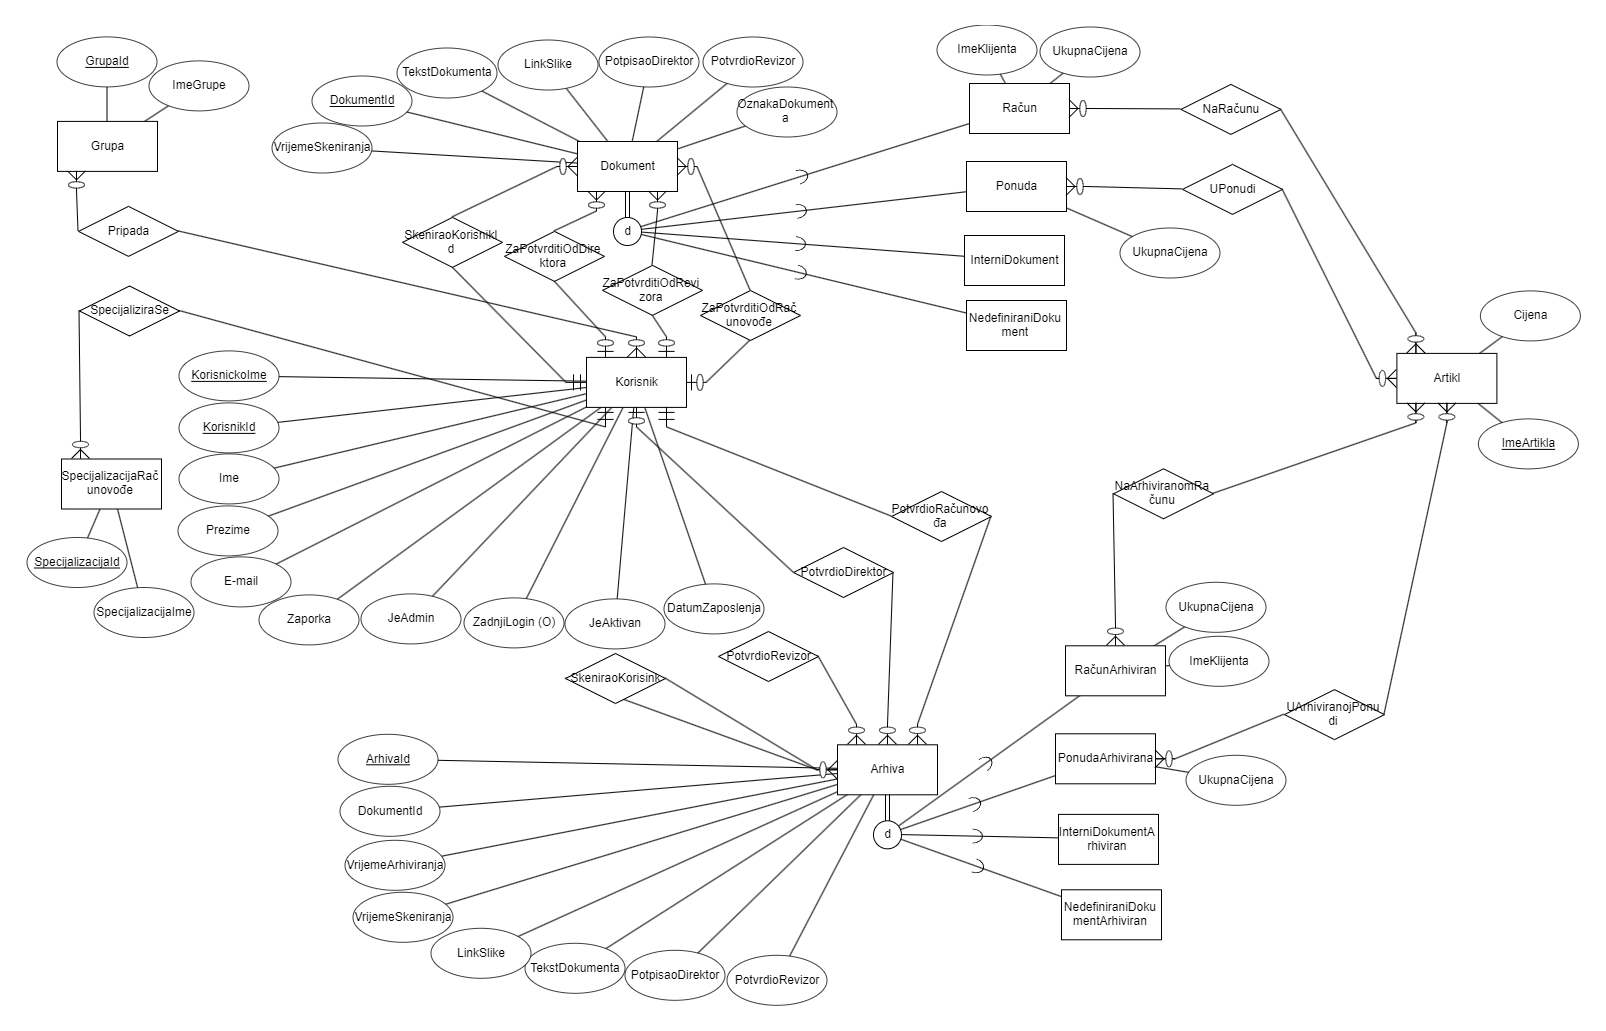
\includegraphics[width=\textwidth]{slike/ER_dijagram.png} %veličina u odnosu na širinu linije
				\caption{ER dijagram baze podataka}
				\label{fig:er_diagram} %label mora biti drugaciji za svaku sliku
			\end{figure}

			\begin{figure}[H]
				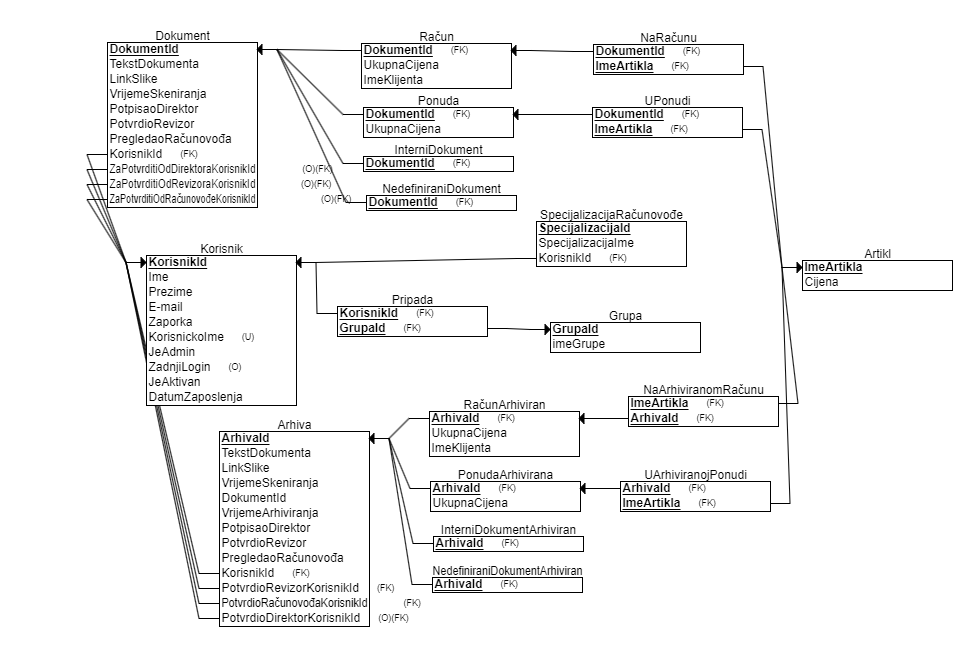
\includegraphics[width=\textwidth]{slike/Relacijska_shema.png} %veličina u odnosu na širinu linije
				\caption{Relacijska shema baze podataka}
				\label{fig:relacijska_shema} %label mora biti drugaciji za svaku sliku
			\end{figure}

			\eject
			
			
		\section{Dijagram razreda}
		
			Na dijagramu razreda Models (slika 4.4) prikazani su razredi unutar datoteke models.py te
			odnosi među njima. U datoteci postoji ukupno 12 razreda. Dokument je nadrazred 4 od tih razreda, a Arhiva
			je također nadrazred 4 od tih razreda.
			\newline
			Dijagram razreda Permissions (slika 4.5) prikazuje razred Permissions,
			koji je nadrazred razredima PripadaDirektorima, PripadaRačunovođama i PripadaRevizorima. Ti se
			razredi nalaze unutar datoteke permissions.py te definiraju kojoj grupi korisnik mora pripadati
			da bi mogao koristiti određeni prikaz web-aplikacije.
			\newline
			Razred Views nalazi se unutar datoteke views.py, u kojoj se također nalazi i razred
			MyTokenObtainPairSerializer kojemu je Views nadrazred. Views koristi taj razred kako bi
			serveru bilo preneseno koje dozvole su prisutne tijekom pokušaja pristupa aplikaciji.
			Na dijagramu razreda Views (slika 4.6) prikazan je odnos između ta dva razreda. 
			
			\begin{figure}[H]
				\
				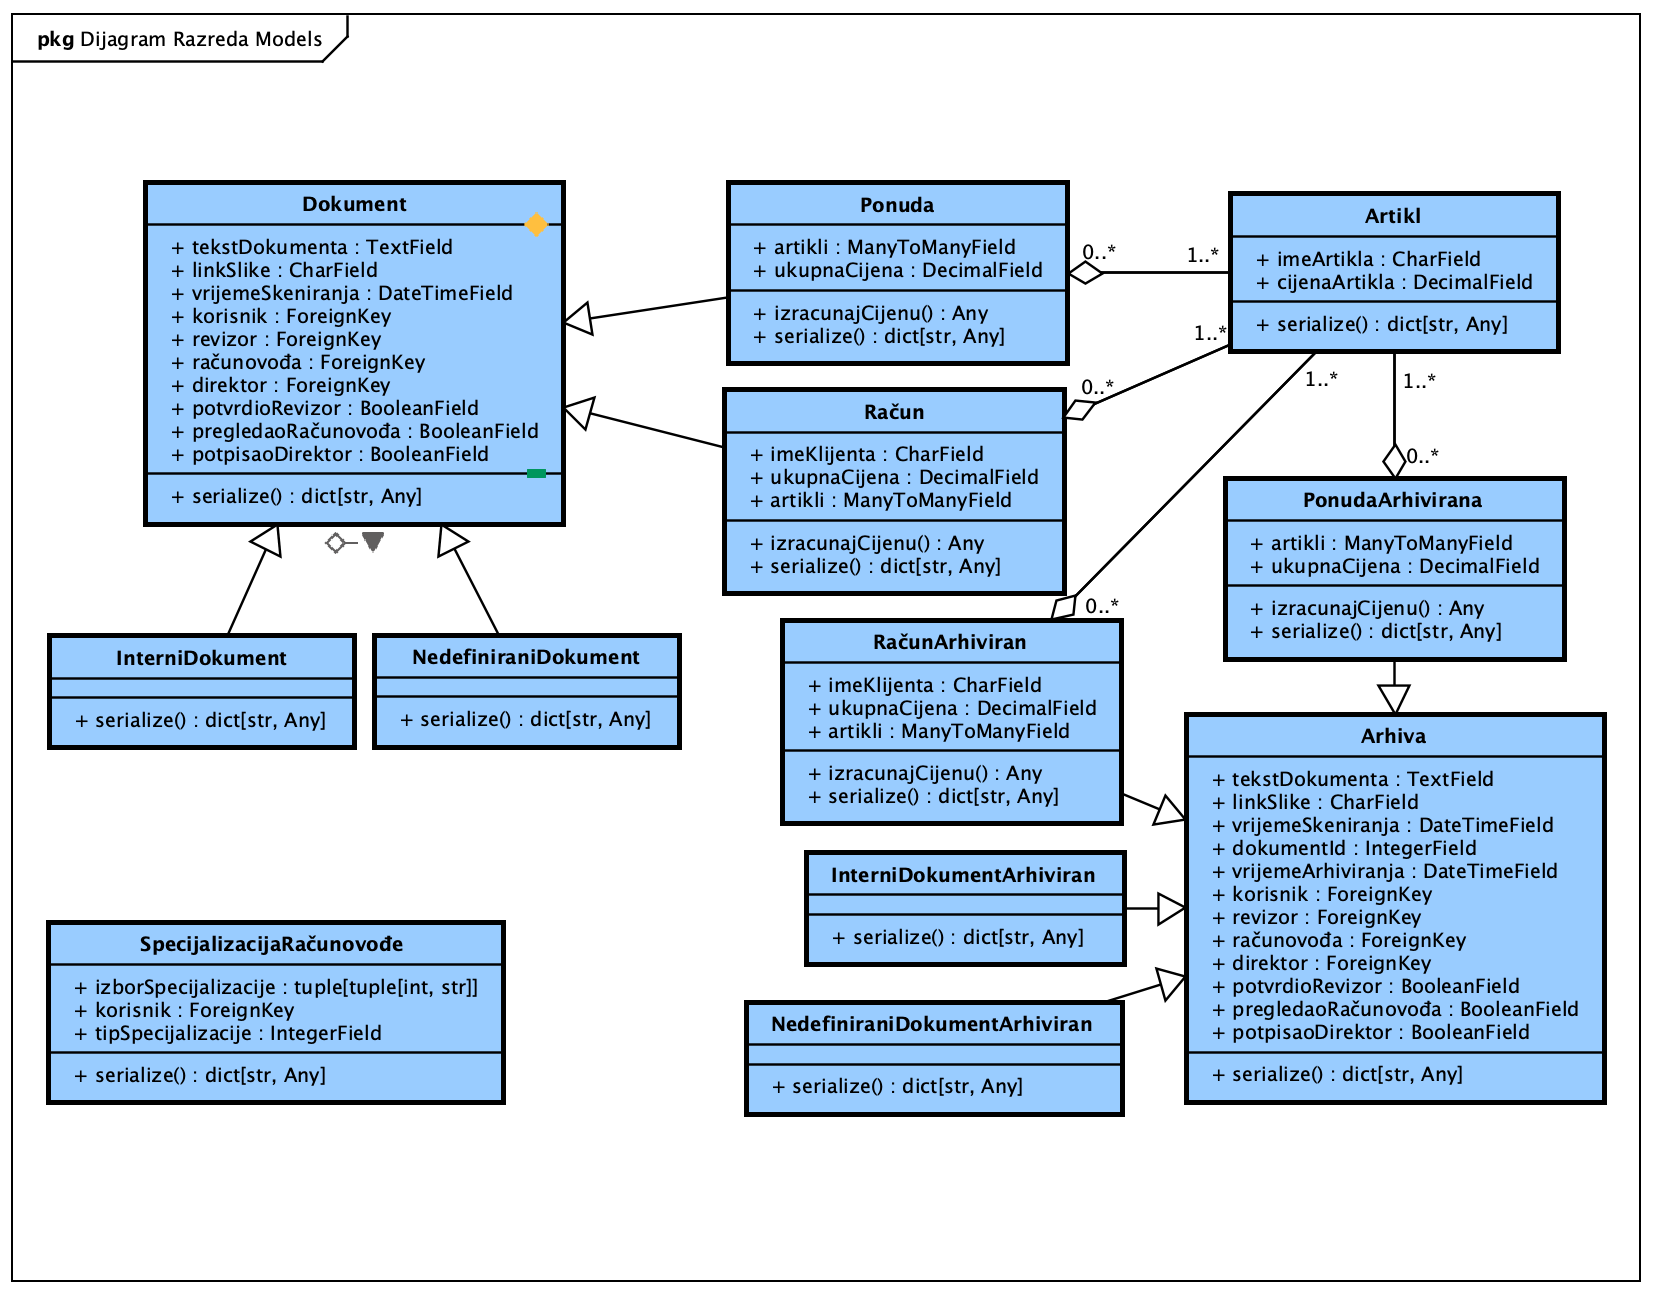
\includegraphics[width=\textwidth]{slike/Class_Models.png}
				\caption{Dijagram razreda - dio Models}
				\label{fig:class_models}
			\end{figure}

			\begin{figure}[H]
				\
				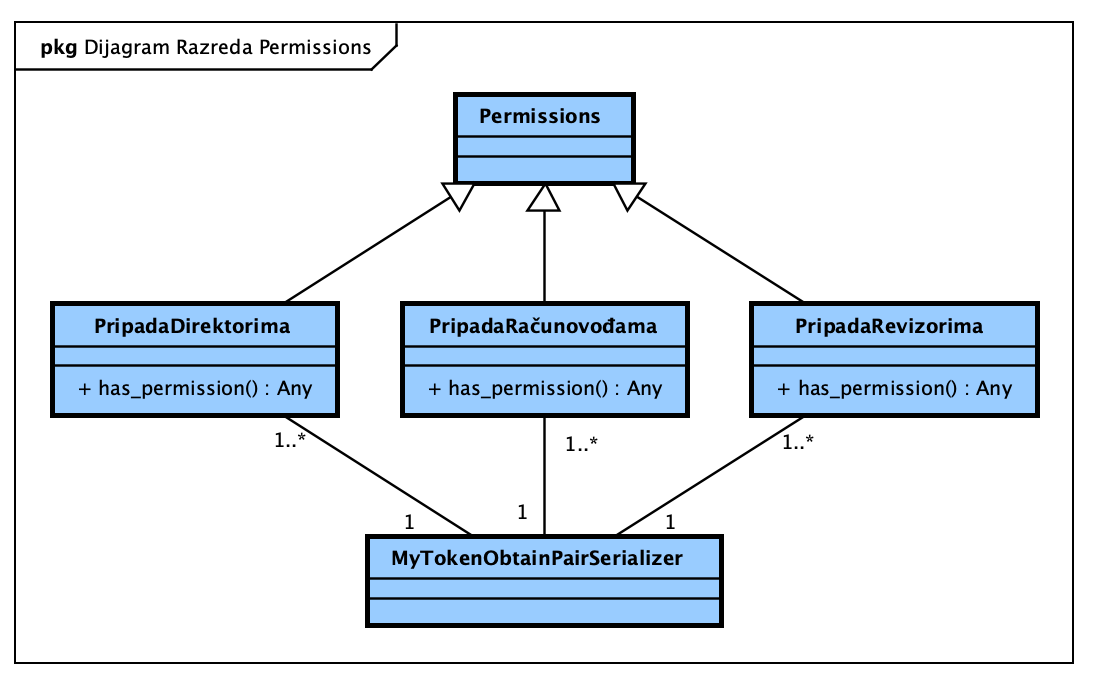
\includegraphics[width=\textwidth]{slike/Class_Permissions.png}
				\caption{Dijagram razreda - dio Permissions}
				\label{fig:class_permissions}
			\end{figure}

			\begin{figure}[H]
				\
				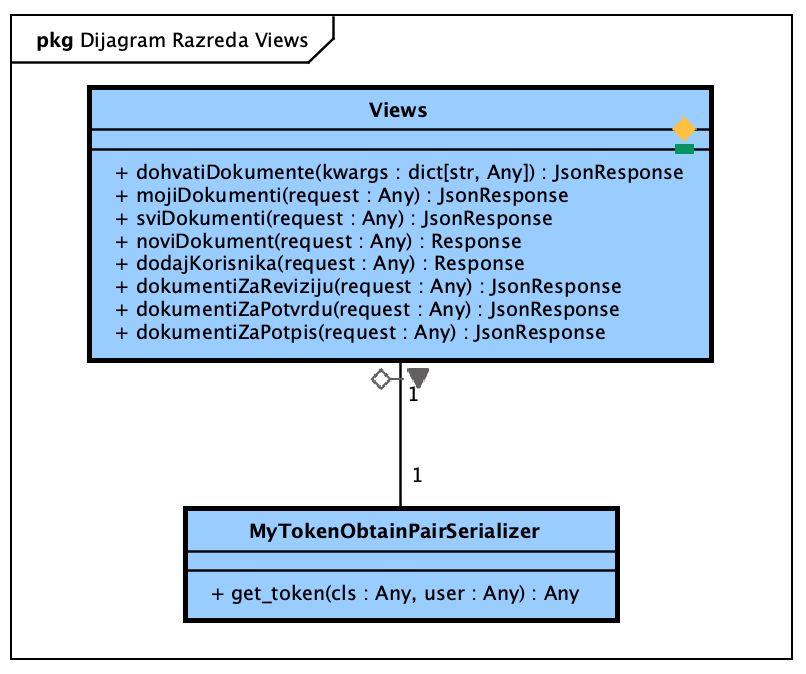
\includegraphics[width=\textwidth]{slike/Class_Views.png}
				\caption{Dijagram razreda - dio Views}
				\label{fig:class_views}
			\end{figure}

			
			\eject
		
		\section{Dijagram stanja}
			
			\begin{figure}[H]
				Na slici 4.7 prikazan je dijagram stanja za direktora nakon obavljene prijave. Prvo što se direktoru prikazuje je početna stranica, koja se također
				prikaže i kada se klikne na "Povijest skeniranja". Klikom na "Skeniraj novi dokument" otvara se prikaz za odabira novog dokumenta s računala te se
				za odabrani dokument nudi opcija njegova učitavanja. Osim toga, s početne se stranice može ući u pregled pristiglih dokumenata te pregled statistike
				dokumenata svakog postojećeg korisnika, koja uključuje dijeljenje dokumenata na jednu od ponuđenih društvenih mreža. Odabirom "Dodaj novog zaposlenika"
				također je moguće dodati i spremiti novog zaposlenika s odgovarajućom ulogom.
				\newline
				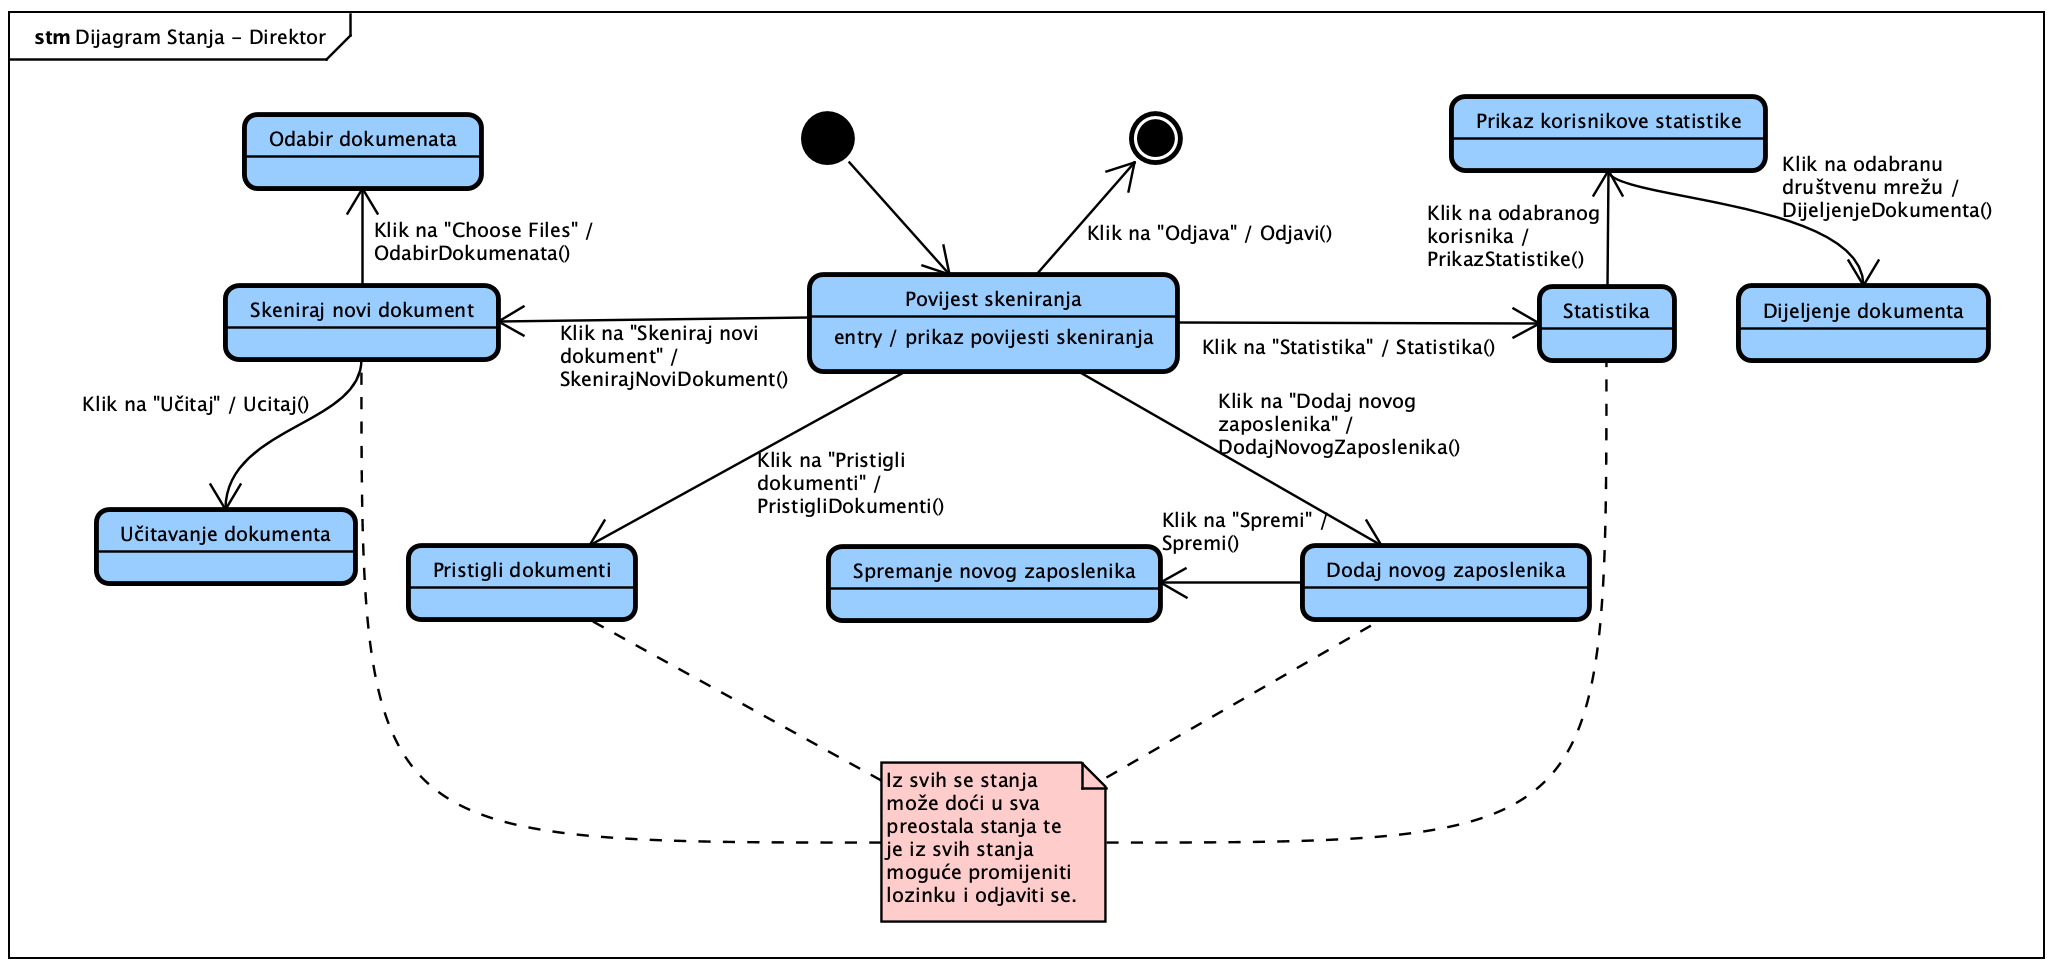
\includegraphics[width=\textwidth]{slike/StateMachine.png}
				\caption{Dijagram stanja}
				\label{fig:StateMachine}
			\end{figure}
			\eject 
		
		\section{Dijagram aktivnosti}
			\begin{figure}[H]
			Dijagramom aktivnosti na slici 4.8 jednostavno je prikazan tok za direktorovu prijavu u sustav te upravljanje dokumentima. Aktivnosti na dijagramu
			odvijaju se slijedno, bez preklapanja. Nakon što se direktor uspješno prijavi u sustav, on dobiva svoj token pomoću kojega web-aplikacija može odrediti
			ulogu prijavljenog korisnika te mu omogućiti odgovarajući prikaz dokumenata. Direktor zatim može napraviti odabranu radnju nad dokumentima između potvrde,
			arhiviranja i potpisivanja. Nakon izvršavanja neke od tih radnji, direktoru se prikazuje ažurirano stanje dokumenata.
			\end{figure}
			\begin{figure}[H]
				\centering
				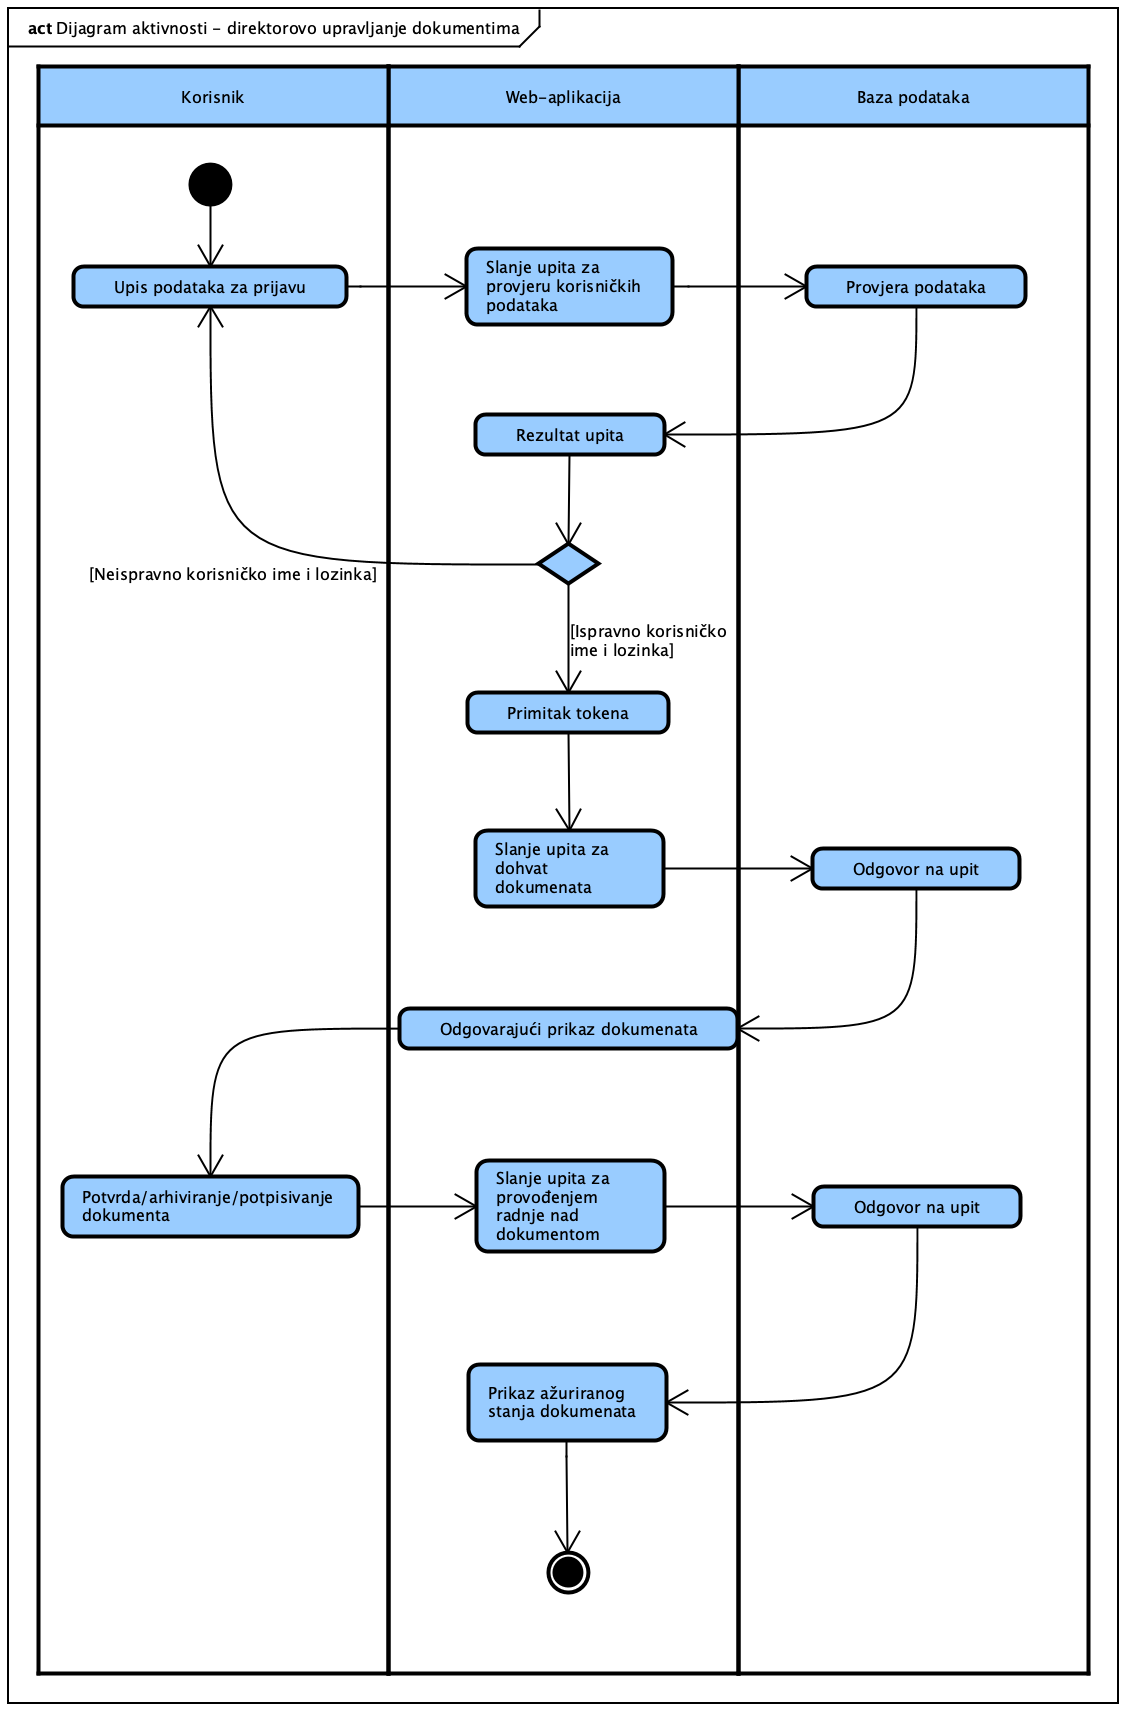
\includegraphics[scale=0.5]{slike/Activity.png}
				\caption{Dijagram aktivnosti}
				\label{fig:Activity}
			\end{figure}
			
			\eject

		\section{Dijagram komponenti}
		
			\begin{figure}[H]
				Na slici 4.9 prikazan je dijagram komponenti. Korisnik pristupa Django backend aplikaciji koristeći React frontend aplikaciju i sučelje REST\_API. Django
				backen aplikacija organizirana je modularno; modul URLs komunicira s modulom Views. On komunicira s modulom Models koji je zadužen za dohvat podataka iz
				baze preko sučelja SQL\_API. Komponenta Hash router unutar React frontend aplikacije na temelju URL-a određuje hoće li se na sučelje poslužiti Login ili
				Main aplikacija. Main aplikacija sastoji se od nekoliko JavaScript datoteka koje određuju prikaze određenih elemenata na stranici za prijavljenog korisnika.
				\newline
				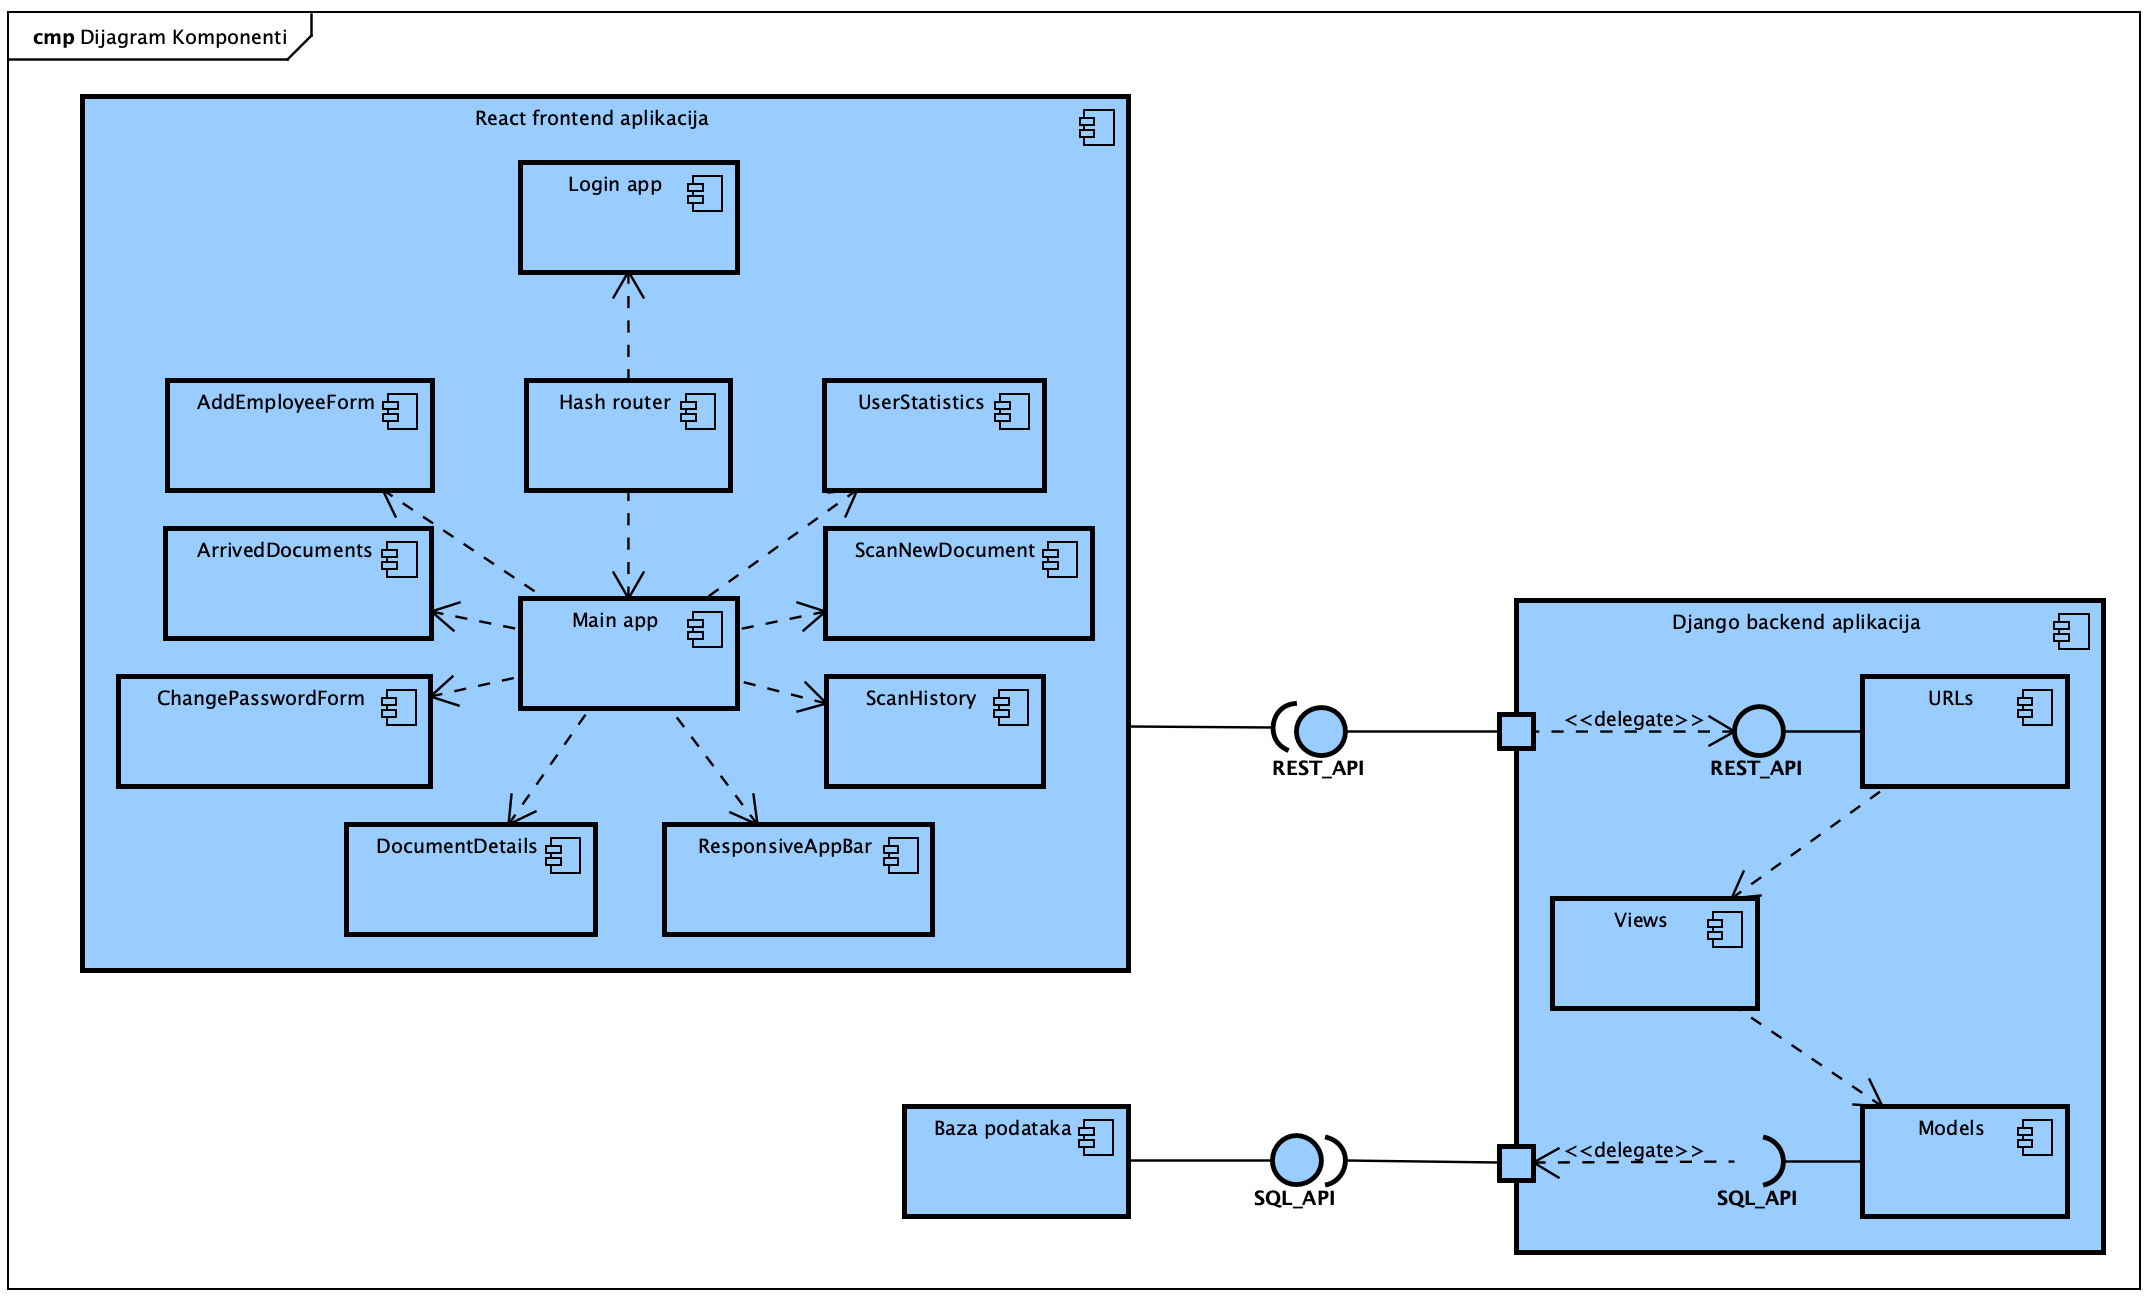
\includegraphics[width=\textwidth]{slike/Component.png}
				\caption{Dijagram komponenti}
				\label{fig:Component}
			\end{figure}
	\chapter{Implementacija i korisničko sučelje}
		
		
		\section{Korištene tehnologije i alati}
		
			
			Svi članovi tima su sudjelovali u odabiru tehnologija i alata koji će se koristiti za izradu aplikacije. Kao sredstvo komunikacije, odabrana je aplikacija 
			\underbar{WhatsApp}\footnote{\url{https://www.whatsapp.com/}}. Pomoću WhatsApp-a, članovi tima su mogli komunicirati u stvarnom vremenu, razmjenjivati datoteke,
			te se dogovarati o terminima sastanaka. Za izradu UML dijagrama korišten je alat \underbar{Astah Professional}\footnote{\url{http://astah.net/editions/professional}}
			dok se \underbar{Git}\footnote{\url{https://git-scm.com/}} koristio kao sustav za upravljanje izvornim kodom. Na web platformi \underbar{GitHub}\footnote{\url{https://github.com/}} je dostupan udaljeni repozitorij projekta.
			Za izradu dokumentacije korišten je \underbar{LaTeX}\footnote{\url{https://www.latex-project.org/}}.
			Za razvojno okruženje korišten je \underbar{Visual Studio Code}\footnote{\url{https://code.visualstudio.com/}} budući da je vrlo popularan za razvoj web i mobilnih aplikacija kao i drugih programa te je vrlo pregledan i jednostavan za korištenje.
			Za izradu naše web aplikacije korišteni su biblioteka \underbar{React}\footnote{\url{https://reactjs.org/}} i jezik \underbar{Javascript}\footnote{\url{https://www.javascript.com/}} za izradu frontenda.
			React je biblioteka za izradu korisničkih sučelja koja je održavana od strane Facebooka. 
			React se koristi za izradu jednostraničnih aplikacija (engl. single-page application) ili mobilnih aplikacija.
			React se fokusira na izradu korisničkog sučelja, dok se za ostale funkcionalnosti aplikacije koristi JavaScript - dinamički tipizirani programski jezik koji je jedan od najpopularnijih na svijetu za izradu web aplikacija.
			Za izradu backenda korišten je jezik \underbar{Python}\footnote{\url{https://www.python.org/}} i biblioteka \underbar{Django}\footnote{\url{https://www.djangoproject.com/}}.
			Django, web framework za Python, poslužio je za razvoj backend dijela aplikacije, dok se za ostale funkcionalnosti koristi Python - još jedan dinamički tipizirani programski jezik često korišten za izradu web aplikacija.

			
			\eject 
		
	
		\section{Ispitivanje programskog rješenja}
			

			\subsection{Ispitivanje komponenti}
\begin{lstlisting}[breaklines=true]
class ViewTest(TestCase):
	def setUp(self):
		Group.objects.create(name='Zaposlenici')
		Group.objects.create(name='Direktori')

		self.base_url = "/api/"
		self.zaposlenik = User.objects.create_user(username='test', password='test')
		Group.objects.get(name='Zaposlenici').user_set.add(self.zaposlenik)
		self.direktor = User.objects.create_user(username='test2', password='test2')
		Group.objects.get(name='Direktori').user_set.add(self.direktor)

		self.client = Client()
		self.zaposlenik_token = self.client.post(self.base_url + 'token/', {'username': 'test', 'password': 'test'}).data.get('access')
		self.direktor_token = self.client.post(self.base_url + 'token/', {'username': 'test2', 'password': 'test2'}).data.get('access')

		self.interni_dokument1 = InterniDokument.objects.create(tekstDokumenta='tekst 1', linkSlike='link 1', vrijemeSkeniranja=timezone.datetime(2021, 5, 5, 10, 10, 10, tzinfo=pytz.UTC), korisnik=self.direktor)
		self.interni_dokument2 = InterniDokument.objects.create(tekstDokumenta='tekst 2', linkSlike='link 2', vrijemeSkeniranja=timezone.datetime(2021, 5, 5, 10, 10, 10, tzinfo=pytz.UTC), korisnik=self.zaposlenik)


	# Testovi funckionalnosti korisnika

	def test_promijeni_lozinku(self):
		self.assertTrue(self.zaposlenik.check_password('test'))

		response = self.client.put(
			self.base_url + 'promijeniLozinku/',
			{"trenutnaLozinka": "test", "novaLozinka": "test"},
			HTTP_AUTHORIZATION='Bearer ' + self.zaposlenik_token,
			content_type='application/json'
		)
		self.assertEquals(response.status_code, 418)

		response = self.client.put(
			self.base_url + 'promijeniLozinku/',
			{"trenutnaLozinka": "test", "novaLozinka": "new_password"},
			HTTP_AUTHORIZATION='Bearer ' + self.zaposlenik_token,
			content_type='application/json'
		)
		self.assertEquals(response.status_code, 200)
		self.zaposlenik.refresh_from_db()
		self.assertFalse(self.zaposlenik.check_password('test'))
		self.assertTrue(self.zaposlenik.check_password('new_password'))

	def test_dodaj_korisnika(self):
		response = self.client.post(
			self.base_url + 'dodajKorisnika/',
			{"username": "test3", "password": "test3"},
			HTTP_AUTHORIZATION='Bearer ' + self.zaposlenik_token,
			content_type='application/json'
		)
		self.assertEquals(response.status_code, 403)

		response = self.client.post(
			self.base_url + 'dodajKorisnika/',
			{"username": "test3", "password": "test3", "email": "abc@example.com", "ime": "test", "prezime": "test", "group": "Zaposlenici"},
			HTTP_AUTHORIZATION='Bearer ' + self.direktor_token,
			content_type='application/json'
		)
		self.assertEquals(response.status_code, 201)
		self.assertTrue(User.objects.filter(username="test3").exists())
		user = User.objects.get(username="test3")
		self.assertTrue(Group.objects.get(name='Zaposlenici').user_set.filter(username="test3").exists())
		self.assertTrue(user.check_password('test3'))
		self.assertEquals(user.email, "abc@example.com")
		self.assertEquals(user.first_name, "test")
		self.assertEquals(user.last_name, "test")
		
	def test_dohvati_korisnike_grupe(self):
		response = self.client.get(
			self.base_url + 'dohvatiKorisnikeGrupe/Zaposlenici',
			HTTP_AUTHORIZATION='Bearer ' + self.zaposlenik_token,
			content_type='application/json'
		)
		
		self.assertEqual(response.status_code, 200)
		data = response.json()
		self.assertEqual(data['korisnici'], [{'id': self.zaposlenik.id, 'username': 'test'}])
		
		response = self.client.get(
			self.base_url + 'dohvatiKorisnikeGrupe/Direktori',
			HTTP_AUTHORIZATION='Bearer ' + self.direktor_token,
			content_type='application/json'
		)
		
		self.assertEqual(response.status_code, 200)
		data = response.json()
		self.assertEqual(data['korisnici'], [{'id': self.direktor.id, 'username': 'test2'}])
		
	def test_dohvati_specijalizirane_racunovodje(self):
		Group.objects.create(name='Računovođe')
		računovođa = User.objects.create_user(username='test3', password='test3')
		Group.objects.get(name='Računovođe').user_set.add(računovođa)

		SpecijalizacijaRačunovođe.objects.create(korisnik=računovođa, tipSpecijalizacije=0)
		
		response = self.client.get(
			self.base_url + 'dohvatiSpecijaliziraneRačunovođe/abc',
			HTTP_AUTHORIZATION='Bearer ' + self.zaposlenik_token,
			content_type='application/json'
		)
		self.assertEqual(response.status_code, 400)
		
		response = self.client.get(
			self.base_url + 'dohvatiSpecijaliziraneRačunovođe/Računi',
			HTTP_AUTHORIZATION='Bearer ' + self.zaposlenik_token,
			content_type='application/json'
		)
		
		self.assertEqual(response.status_code, 200)
		data = response.json()
		self.assertEqual(data['korisnici'], [{'id': računovođa.id, 'username': 'test3'}])
		
		response = self.client.get(
			self.base_url + 'dohvatiSpecijaliziraneRačunovođe/Ponude',
			HTTP_AUTHORIZATION='Bearer ' + self.zaposlenik_token,
			content_type='application/json'
		)
		
		self.assertEqual(response.status_code, 200)
		data = response.json()
		self.assertEqual(data['korisnici'], [])
		
		
	# Testovi funkcionalnosti rada s dokumentima
	
	def test_moji_dokumenti(self):
		response = self.client.get(
			self.base_url + 'mojiDokumenti/',
			HTTP_AUTHORIZATION='Bearer ' + self.direktor_token,
			content_type='application/json'
		)
		self.assertEqual(response.status_code, 200)
		data = response.json()
		self.assertEqual(len(data['dokumenti']), 1)
		self.assertEqual(data['dokumenti'][0]['id'], self.interni_dokument1.id)
		
	def test_svi_dokumenti(self):
		response = self.client.get(
			self.base_url + 'sviDokumenti/',
			HTTP_AUTHORIZATION='Bearer ' + self.direktor_token,
			content_type='application/json'
		)
		self.assertEqual(response.status_code, 200)
		data = response.json()
		self.assertEqual(len(data['dokumenti']), 2)
		self.assertEqual(data['dokumenti'][0]['id'], self.interni_dokument1.id)
		self.assertEqual(data['dokumenti'][1]['id'], self.interni_dokument2.id)

	def test_označi_točnost_skeniranja(self):
		self.assertFalse(self.interni_dokument2.točnoSkeniran)
		response = self.client.put(
			self.base_url + 'označiTočnostSkeniranja/' + str(self.interni_dokument2.id),
			{"tocnost": True},
			HTTP_AUTHORIZATION='Bearer ' + self.zaposlenik_token,
			content_type='application/json'
		)
		self.assertEqual(response.status_code, 200)
		self.interni_dokument2.refresh_from_db()
		self.assertTrue(self.interni_dokument2.točnoSkeniran)
		
	def test_potpiši(self):
		self.assertFalse(self.interni_dokument1.potpisaoDirektor)
		response = self.client.put(
			self.base_url + 'potpiši/' + str(self.interni_dokument1.id),
			HTTP_AUTHORIZATION='Bearer ' + self.direktor_token,
			content_type='application/json'
		)
		
		self.assertEqual(response.status_code, 200)
		self.interni_dokument1.refresh_from_db()
		self.assertTrue(self.interni_dokument1.potpisaoDirektor)
		
	def test_dodijeli_revizora(self):
		revizori = Group.objects.create(name='Revizori')
		revizor = User.objects.create_user(username='test3', password='test3')
		revizori.user_set.add(revizor)
		
		self.assertIsNone(self.interni_dokument1.revizor)
		response = self.client.put(
			self.base_url + 'dodijeliRevizora/' + str(self.interni_dokument1.id),
			{"korisnik_id": revizor.id},
			HTTP_AUTHORIZATION='Bearer ' + self.zaposlenik_token,
			content_type='application/json'
		)
		
		self.assertEqual(response.status_code, 200)
		self.interni_dokument1.refresh_from_db()
		self.assertEqual(self.interni_dokument1.revizor, revizor)
		
		response = self.client.put(
			self.base_url + 'dodijeliRevizora/' + str(self.interni_dokument1.id),
			{"korisnik_id": self.direktor.id},
			HTTP_AUTHORIZATION='Bearer ' + self.zaposlenik_token,
			content_type='application/json'
		)
		self.assertEqual(response.status_code, 400)
		
		response = self.client.put(
			self.base_url + 'dodijeliRevizora/' + '0',
			{"korisnik_id": revizor.id},
			HTTP_AUTHORIZATION='Bearer ' + self.zaposlenik_token,
			content_type='application/json'
		)
		self.assertEqual(response.status_code, 404)
		
	def test_arhiviraj(self):
		Group.objects.create(name='Računovođe')
		računovođa = User.objects.create_user(username='test3', password='test3')
		Group.objects.get(name='Računovođe').user_set.add(računovođa)
		
		računovođa_token = self.client.post(self.base_url + 'token/', {'username': 'test3', 'password': 'test3'}).data.get('access')
		
		pk = self.interni_dokument1.pk
		tekst = self.interni_dokument1.tekstDokumenta
		self.assertTrue(InterniDokument.objects.filter(pk=pk).exists())
		self.assertFalse(InterniDokumentArhiviran.objects.filter(dokumentId=pk).exists())
		response = self.client.put(
			self.base_url + 'arhiviraj/' + str(self.interni_dokument1.id),
			HTTP_AUTHORIZATION='Bearer ' + računovođa_token,
			content_type='application/json'
		)

		self.assertEqual(response.status_code, 200)
		self.assertFalse(InterniDokument.objects.filter(pk=pk).exists())
		
		documents = InterniDokumentArhiviran.objects.filter(dokumentId=pk)
		self.assertTrue(documents.exists())
		self.assertTrue(len(documents) == 1)
		self.assertTrue(documents[0].tekstDokumenta == tekst)
		
		
Rezultat izvođenja u vscodeu:
Found 10 test(s).
Creating test database for alias 'default'...
System check identified no issues (0 silenced).
..........
----------------------------------------------------------------------
Ran 10 tests in 11.969s

OK
Destroying test database for alias 'default'...
\end{lstlisting}
			
			
			\subsection{Ispitivanje sustava}
			
			Test 1 (test\_login\_fail):\\
			Otvorimo URI web stranice. Pokušamo se ulogirati s neispravnom kombinacijom korisničkog imena i zaporke.
			Osiguramo da se pojavi alert s tekstom "Pogrešno korisničko ime ili lozinka".\\
			\\
			Test 2 (test\_login\_and\_logout):\\
			Otvorimo URI web stranice. Ulogiramo se s ispravnim korisničkim imenom i lozinkom. Izlogiramo se.
			Osiguramo da smo opet završili na login stranici.\\
			\\
			Test 3 (test\_change\_password):\\
			Otvorimo URI web stranice. Ulogiramo se s ispravnim korisničkim imenom i lozinkom. Pokušamo promijeniti
			lozinku korisnika pri čemu unesemo pogrešnu trenutnu lozinku. Osiguramo da se pojavi alert teksta
			"Unesite ispravnu trenutnu lozinku" i da se lozinka korisnika nije promijenila. Ponovimo isto ali s
			ispravnom trenutnom lozinkom i novom lozinkom istom kao i starom. Osiguramo da se pojavi alert teksta
			"Nova lozinka mora biti različita od stare" i da se lozinka korisnika nije promijenila. Ponovimo isto s
			ispravnom trenutnom lozinkom i novom lozinkom različitom od stare. Osiguramo da se pojavio alert teksta
			"Lozinka uspješno promijenjena" i da lozinka korisnika promijenila. Vratimo lozinku na staru.\\
			\\
			Test 4 (test\_add\_new\_employee):\\
			Otvorimo URI web stranice. Ulogiramo se s ispravnim direktorovim korisničkim imenom i lozinkom.
			Otvorimo stranicu za dodavanje novog zaposlenika. Pokušamo dodati novog zaposlenika s istim korisničkim
			imena kao neki već postojeći. Osiguramo da se pojavi alert teksta "Greška prilikom dodavanja zaposlenika".
			Ponovimo isto ali s ispravim korisničkim imenom. Osiguramo da se pojavi alert teksta "Zaposlenik uspješno
			dodan". Osiguramo da se novi korisnik pojavio u bazi sa svim potrebnim atributima. Izbrišemo novonastalog
			korisnika.
			
			\eject 
		
		
		\section{Dijagram razmještaja}
			
			\begin{figure}[H]
				Dijagram razmještaja na slici 5.1 prikazuje topologiju sklopovlja i programsku potporu web-aplikacije. Sustav je baziran na arhitekturi
				"klijent-poslužitelj". Komunikacija između računala korisnika i frontend poslužiteljskog računala, kao i između frontend i backend poslužiteljskog
				računala, odvija se preko HTTP veze. Korisnici pristupaju web-aplikaciji koristeći web preglednik te im frontend poslužiteljsko računalo, na kojem
				se nalazi frontend web poslužitelj, daje odgovarajući prikaz. Na backend poslužiteljskom računalu nalazi se Docker u kojemu se nalaze backend web
				poslužitelj i Tesseract, a Postgres baza nalazi se na poslužiteljskom računalu baze podataka koje je povezano s backend poslužiteljskim računalom.
				\newline
				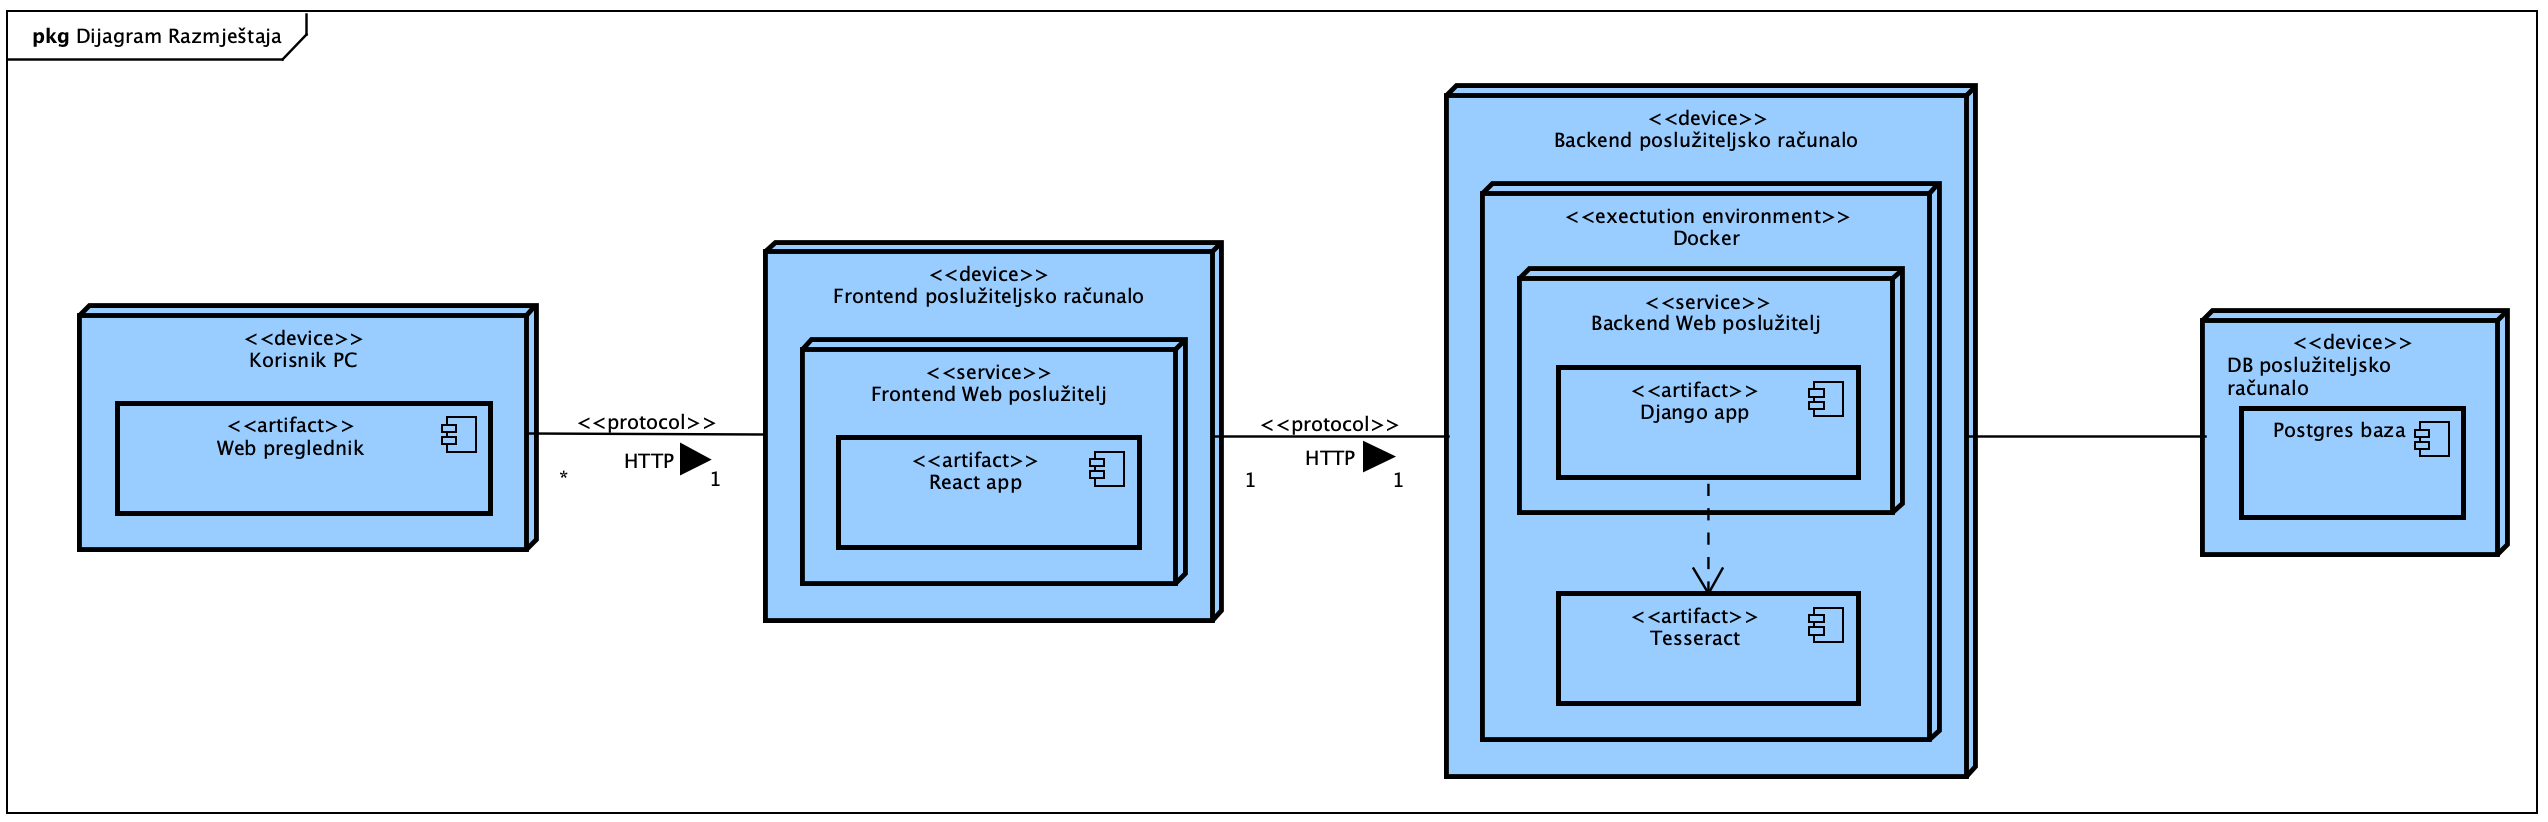
\includegraphics[width=\textwidth]{slike/Deployment.png}
				\caption{Dijagram razmještaja}
				\label{fig:Deployment}
			\end{figure}
			\eject 
		
		\section{Upute za puštanje u pogon}
		
			\subsubsection{Baza Podataka}

			Za puštanje web aplikacije u pogon potrebno je prvo pronaći online uslugu koji pruža uslugu posluživanja baze podataka.

			Na tom servisu potrebno je stvoriti novu PostgreSQL bazu te korisnika koji ima pristup bazi. Nije potrebno inicijalizirati
			tablice u bazi. Potreban je samo URL.

			\begin{figure}[H]
				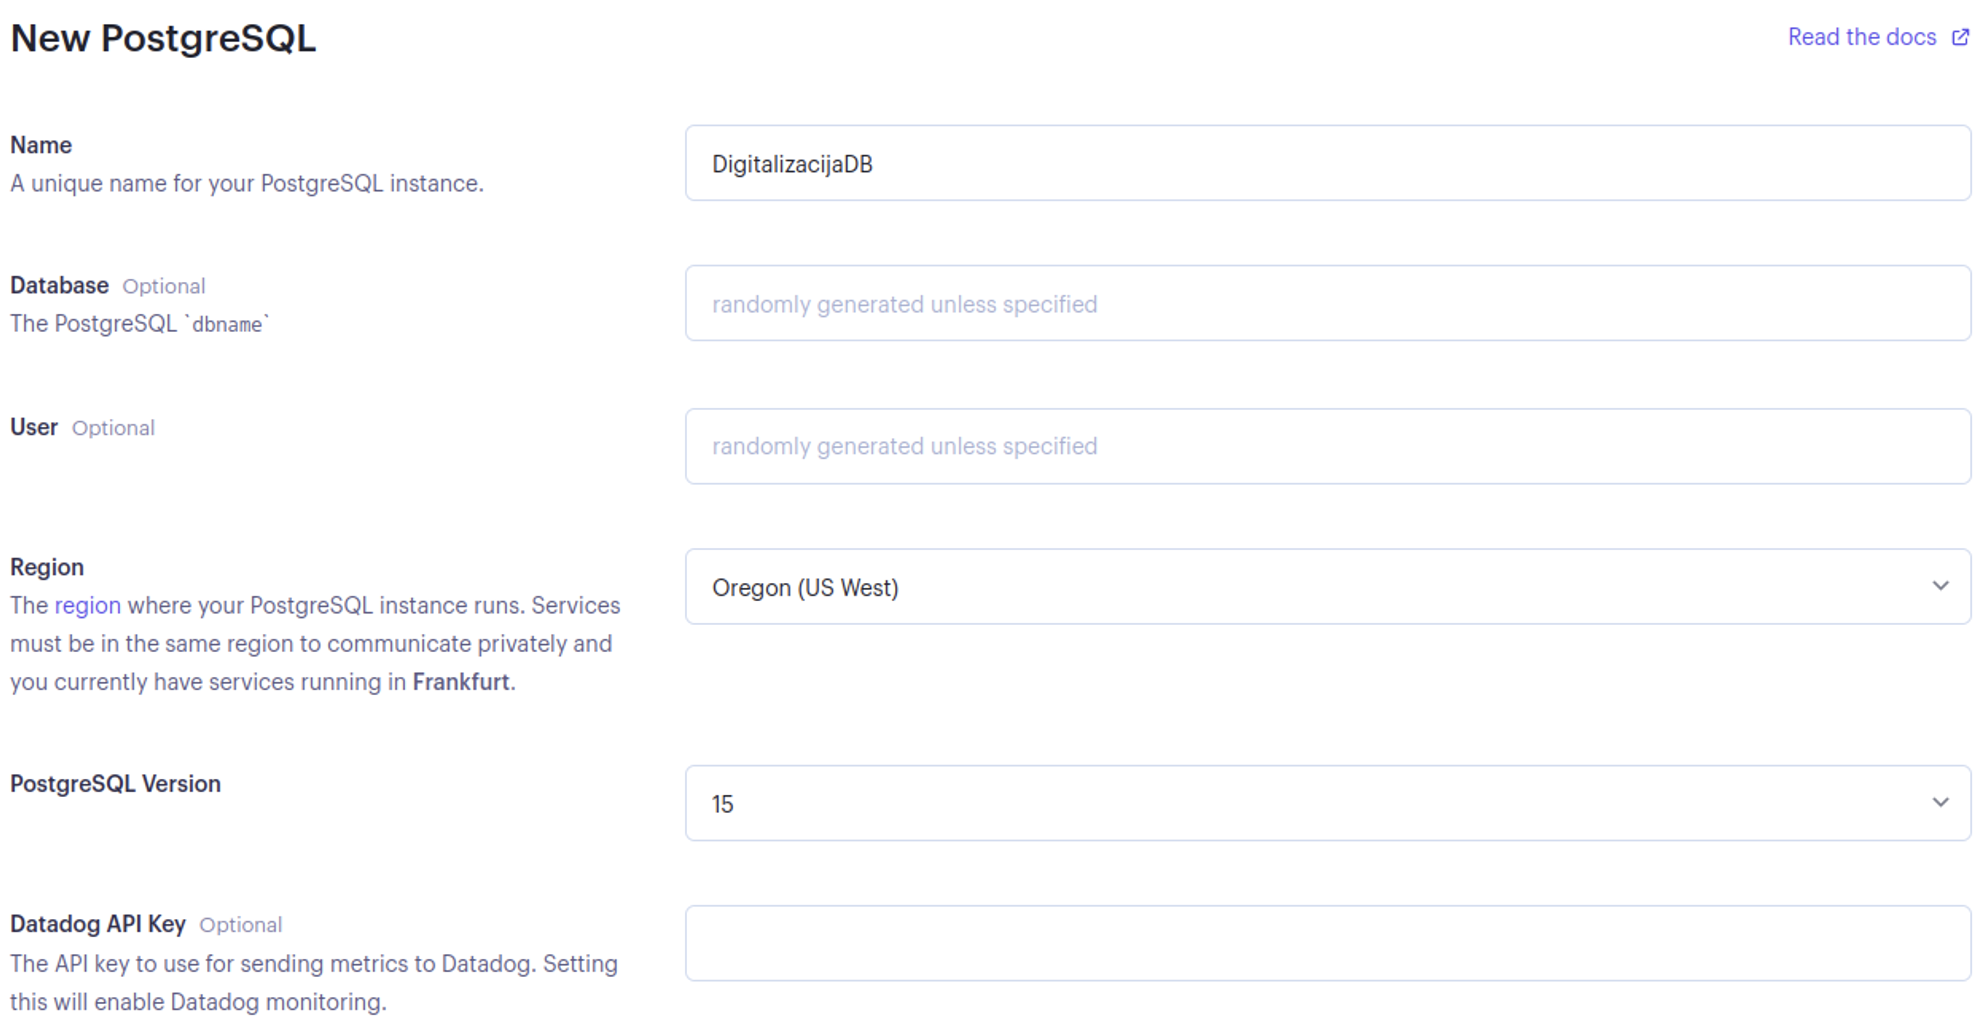
\includegraphics[width=\textwidth]{slike/creatingDB.png}
				\caption{Primjer stvaranja baze podataka na render.com}
				\label{fig:stvaranje_baze}
			\end{figure}


			\subsubsection{Backend}

			Za puštanje backenda u pogon potrebno je na Git-u podesiti datoteku „IzvorniKod/Digitalizacija/Digitalizacija/.env“
			tako da u njoj postavite varijablu okoline DATABASE_URL na URL baze podataka stvorene u prijašnjem koraku.

			\begin{figure}[H]
				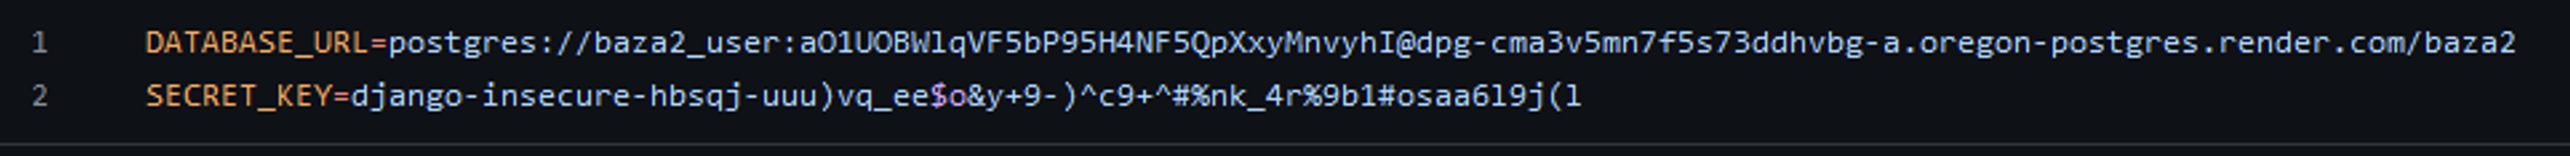
\includegraphics[width=\textwidth]{slike/envFile.png}
				\caption{Primjer .env datoteke}
				\label{fig:env_datoteka}
			\end{figure}

			Nakon toga potrebno je pronaći uslugu koji omogućava puštanje web servisa u pogon na temelju Dockerfile-a na Git-u.
			Bitno je da korijenski direktorij iz kojeg pogonimo ovaj servis bude postavljen na „IzvorniKod/Digitalizacija/“. 

			\begin{figure}[H]
				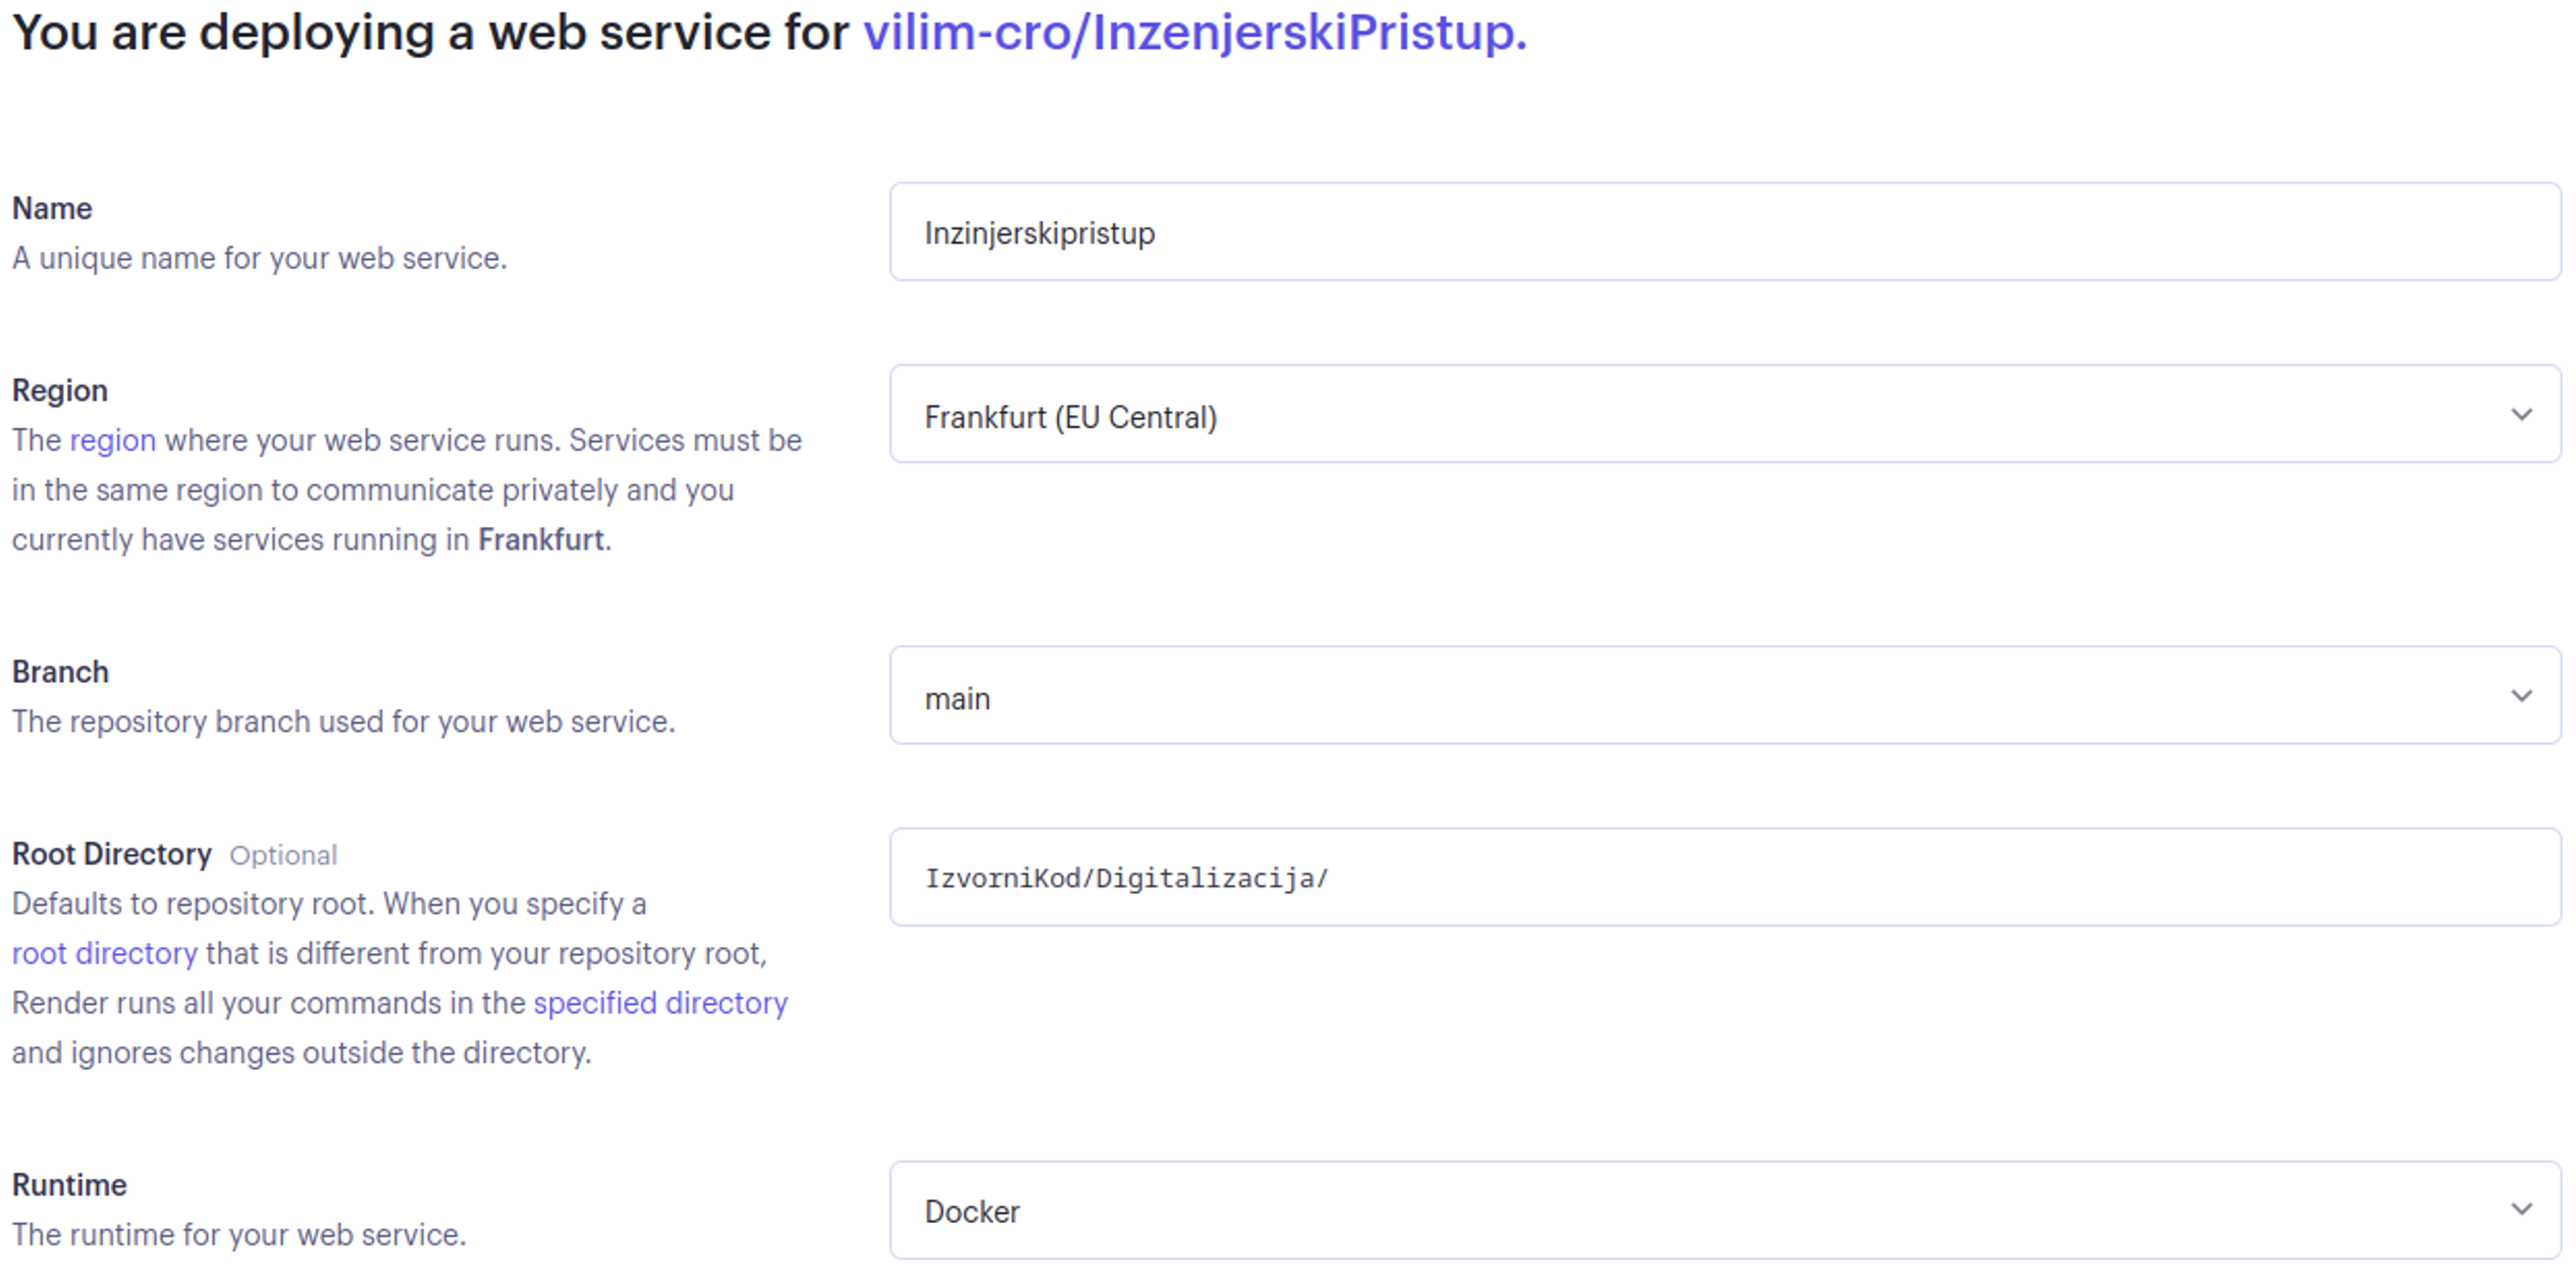
\includegraphics[width=\textwidth]{slike/deployingBackend.png}
				\caption{Primjer puštanja backenda u pogon na render.com}
				\label{fig:deploying-backend}
			\end{figure}

			Jednom kad smo postavili sve postavke, web usluga će na temelju Dockerfile-a upogoniti backend.

			Ako želimo backend uslugu pokrenuti lokalno, potrebno je instalirati docker. On se može instalirati prema uputama
			koje se mogu naći ovdje https://docs.docker.com/get-docker/.
			Nakon toga, potrebno je klonirati sadržaj prije navedenog direktorija te u njemu pokrenuti naredbu
			„docker build -t digitalizacija .“ te pričekati da se izgradi slika. Nakon toga backend možemo pokrenuti naredbom
			„docker run -p 8000:8000 digitalizacija“.

			\begin{figure}[H]
				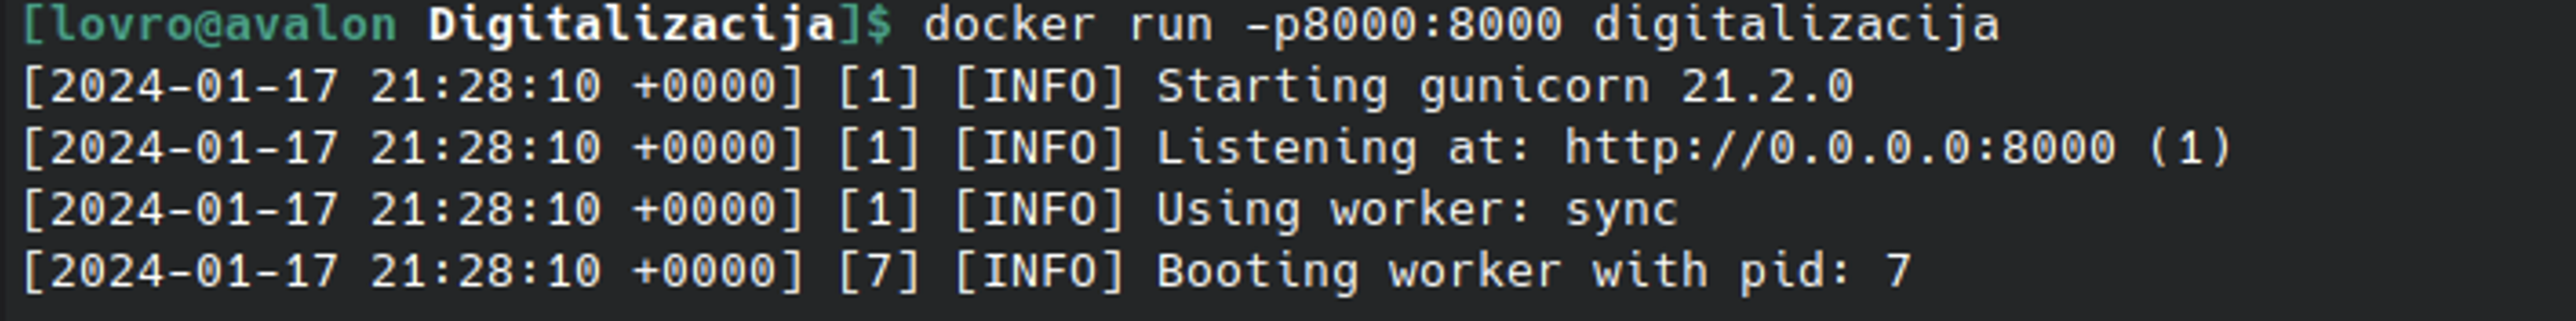
\includegraphics[width=\textwidth]{slike/runBackendLocal.png}
				\caption{Primjer lokalnog pokretanja backenda}
				\label{fig:lokalno-pokretanje-backenda}
			\end{figure}


			\subsubsection{Frontend}

			Za puštanje frontenda u pogon potrebno je pronaći web uslugu koja može posluživati našu React web aplikaciju.

			Potrebno je kao korijenski direktorij postaviti „IzvorniKod/reactapp/“ te osigurati da se pri pokretanju koriste
			naredbe „npm install“ te „npm run build“. Izvršnu izgradnju možemo jednostavno staviti u direktorij „build“. 

			\begin{figure}[H]
				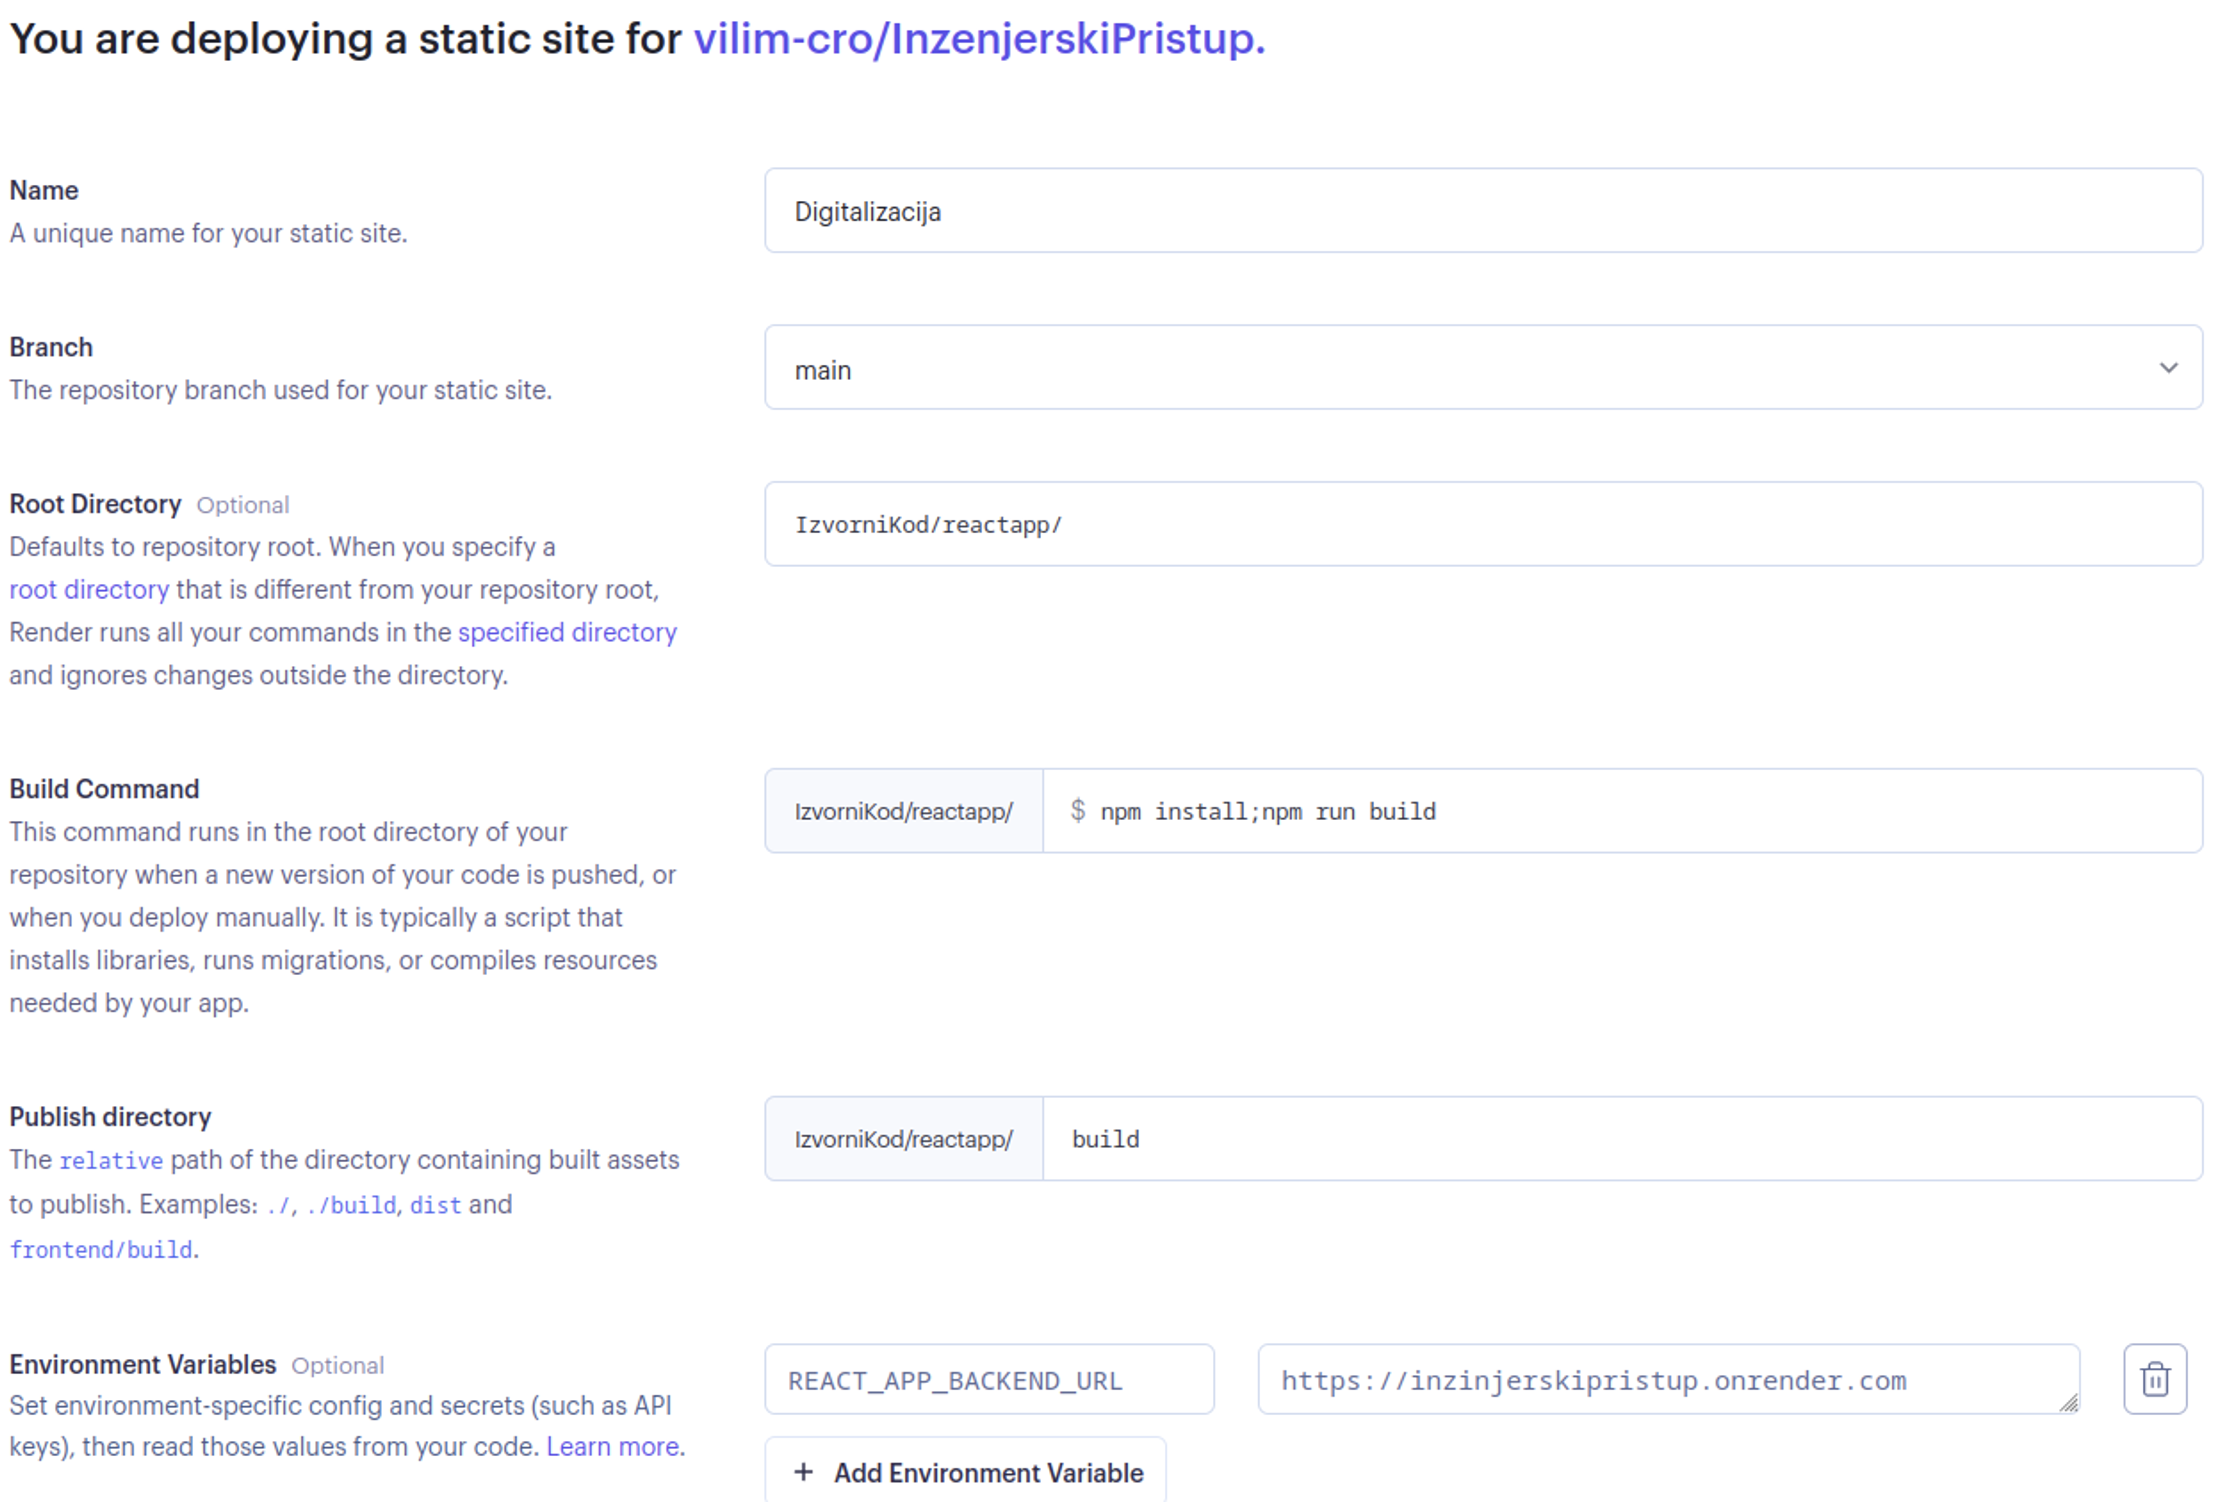
\includegraphics[width=\textwidth]{slike/deployingFrontend.png}
				\caption{Primjer puštanja frontenda u pogon na render.com}
				\label{fig:lokalno-pokretanje-backenda}
			\end{figure}

			Konačno, prije puštanja frontenda u pogon, moramo mu putem varijable okoline REACT_APP_BACKEND_URL prenijeti URL
			backenda koji smo stvorili u prošlom koraku.

			Ako želimo frontend pokrenuti lokalno potrebno je prvo instalirati node.js i npm. Njih možemo instalirati prema ovim
			uputama https://docs.npmjs.com/downloading-and-installing-node-js-and-npm.
			Nakon toga potrebno je klonirati sadržaj direktorija „IzvorniKod/reactapp/“ na Git-u. Također je potrebno u ljusci
			postaviti varijablu okoline te pokrenuti naredbe „npm install“ i „npm run build“. Frontend sada možemo pokrenuti
			naredbom „serve -s build“. 

			Nakon toga na URL-u na kojem smo pogonili frontend možemo pristupiti aplikaciji.
			
			\eject 
	\chapter{Zaključak i budući rad}
		
		\textbf{\textit{dio 2. revizije}}\\
		
		 \textit{U ovom poglavlju potrebno je napisati osvrt na vrijeme izrade projektnog zadatka, koji su tehnički izazovi prepoznati, jesu li riješeni ili kako bi mogli biti riješeni, koja su znanja stečena pri izradi projekta, koja bi znanja bila posebno potrebna za brže i kvalitetnije ostvarenje projekta i koje bi bile perspektive za nastavak rada u projektnoj grupi.}
		
		 \textit{Potrebno je točno popisati funkcionalnosti koje nisu implementirane u ostvarenoj aplikaciji.}
		
		\eject 
	\chapter*{Popis literature}
		\addcontentsline{toc}{chapter}{Popis literature}
	 	
 		
		
		\begin{enumerate}
			
			
			\item  Programsko inženjerstvo, FER ZEMRIS, \url{http://www.fer.hr/predmet/proinz}
			
			\item  I. Sommerville, "Software engineering", 8th ed, Addison Wesley, 2007.
			
			\item  T.C.Lethbridge, R.Langaniere, "Object-Oriented Software Engineering", 2nd ed. McGraw-Hill, 2005.
			
			\item  I. Marsic, Software engineering book``, Department of Electrical and Computer Engineering, Rutgers University, \url{http://www.ece.rutgers.edu/~marsic/books/SE}
			
			\item  The Unified Modeling Language, \url{https://www.uml-diagrams.org/}
			
			\item  Astah Community, \url{http://astah.net/editions/uml-new}
			
			\item CS50’s Web Programming with Python and JavaScript, \url{https://cs50.harvard.edu/web/2020/weeks/3/}
			
			\item Django, \url{https://www.djangoproject.com/}
			
			\item React Course - Beginner's Tutorial for React JavaScript Library [2022], \url{https://www.youtube.com/watch?v=bMknfKXIFA8}
			
			\item Stack overflow, \url{https://stackoverflow.com/}
		\end{enumerate}
		
		 
	
	
	\begingroup
	\renewcommand*\listfigurename{Indeks slika i dijagrama}
	%\renewcommand*\listtablename{Indeks tablica}
	%\let\clearpage\relax
	\listoffigures
	%\vspace{10mm}
	%\listoftables
	\endgroup
	\addcontentsline{toc}{chapter}{Indeks slika i dijagrama}


	
	\eject{}
		
	\chapter*{Dodatak: Prikaz aktivnosti grupe}
		\addcontentsline{toc}{chapter}{Dodatak: Prikaz aktivnosti grupe}
		
		\section*{Dnevnik sastajanja}
		
		
		
		\begin{packed_enum}
			\item  sastanak
			
			\item[] \begin{packed_item}
				\item Datum: 20.\ listopada 2023.
				\item Prisustvovali: svi
				\item Teme sastanka:
				\begin{packed_item}
					\item  odabir razvojnih alata i tehnologija
					\item  generalna podjela poslova
				\end{packed_item}
			\end{packed_item}
			
			\item  sastanak
			\item[] \begin{packed_item}
				\item Datum: 25.\ listopada 2023.
				\item Prisustvovali: svi
				\item Teme sastanka:
				\begin{packed_item}
					\item  detaljnija podjela poslova
					\item  rasprava oko funkcionalnih i nefunkcionalnih zahtjeva
				\end{packed_item}
			\end{packed_item}

			\item  sastanak
			\item[] \begin{packed_item}
				\item Datum: 26.\ listopada 2023.
				\item Prisustvovali: Filip Krilčić, Vilim Branica, Lovro Mužar
				\item Teme sastanka:
				\begin{packed_item}
					\item  organizacija baze podataka
					\item  dijagrami i implementacija baze podataka
				\end{packed_item}
			\end{packed_item}
			
			\item  sastanak
			\item[] \begin{packed_item}
				\item Datum: 27.\ listopada 2023.
				\item Prisustvovali: Filip Krilčić, Vilim Branica, Zvonimir Pipić, Nika Miličević, Marko Šelendić, Lovro Mužar
				\item Teme sastanka:
				\begin{packed_item}
					\item  završavanje prošlo podijeljenih poslova te provjera prethodno završenog posla
					\item  podijela novih poslova - OCR demo, dokumentacija (Sekvencijski dijagrami te opis projekta), opis baze i početna stranica, te određivanje roka za završetak istih
				\end{packed_item}
			\end{packed_item}
			
			\item  sastanak
			\item[] \begin{packed_item}
				\item Datum: 28.\ listopada 2023.
				\item Prisustvovali: Filip Krilčić, Vilim Branica i Zvonimir Pipić
				\item Teme sastanka:
				\begin{packed_item}
					\item  podjela poslova na backendu
				\end{packed_item}
			\end{packed_item}
			
			\item  sastanak
			\item[] \begin{packed_item}
				\item Datum: 4.\ studenoga 2023.
				\item Prisustvovali: Filip Krilčić, Vilim Branica, Zvonimir Pipić, Nika Miličević, Marko Šelendić, Tomislav Čupić
				\item Teme sastanka:
				\begin{packed_item}
					\item  analiza commitanih fileova
					\item  prezentacija izrađenih osnovnih funkcionalnosti backenda
				\end{packed_item}
			\end{packed_item}

			\item  sastanak
			\item[] \begin{packed_item}
				\item Datum: 12.\ prosinca 2023.
				\item Prisustvovali: svi
				\item Teme sastanka:
				\begin{packed_item}
					\item  podjela bodova 1. revizije
					\item  analiza riješenih zadataka
					\item  određivanje preostalih zadataka 
				\end{packed_item}
			\end{packed_item}

   			\item  sastanak
			\item[] \begin{packed_item}
				\item Datum: 16.\ prosinca 2023.
				\item Prisustvovali: Marko Šelendić, Tomislav Čupić, Zvonimir Pipić
				\item Teme sastanka:
				\begin{packed_item}
					\item  podjela poslova na frontendu
				\end{packed_item}
			\end{packed_item}

			\item  sastanak
			\item[] \begin{packed_item}
				\item Datum: 13.\ siječnja 2024.
				\item Prisustvovali: svi
				\item Teme sastanka:
				\begin{packed_item}
					\item  pregled svih napravljenih funkcionalnosti, provjera rada aplikacije i ispravljanje sitnih grešaka 
				\end{packed_item}
			\end{packed_item}

		\end{packed_enum}
		
		\eject{}
		\section*{Tablica aktivnosti}
		
			\textbf{\textit{Kontinuirano osvježavanje}}\\
			
			 \textit{Napomena: Doprinose u aktivnostima treba navesti u satima po članovima grupe po aktivnosti.}

			\begin{longtblr}[
					label=none,
				]{
					vlines,hlines,
					width = \textwidth,
					colspec={X[7, l]X[1, c]X[1, c]X[1, c]X[1, c]X[1, c]X[1, c]X[1, c]}, 
					vline{1} = {1}{text=\clap{}},
					hline{1} = {1}{text=\clap{}},
					rowhead = 1,
				} 
			
				\SetCell[c=1]{c}{} & \SetCell[c=1]{c}{\rotatebox{90}{\textbf{Vilim Branica}}} & \SetCell[c=1]{c}{\rotatebox{90}{\textbf{Tomislav Čupić}}} &	\SetCell[c=1]{c}{\rotatebox{90}{\textbf{Filip Krilčić}}} & \SetCell[c=1]{c}{\rotatebox{90}{\textbf{Nika Miličević}}} &	\SetCell[c=1]{c}{\rotatebox{90}{\textbf{Lovro Mužar}}} & \SetCell[c=1]{c}{\rotatebox{90}{\textbf{Zvonimir Pipić}}} &	\SetCell[c=1]{c}{\rotatebox{90}{\textbf{Marko Šelendić}}} \\  
				Upravljanje projektom 		& 6 &  &  &  &  &  & \\ 
				Opis projektnog zadatka 	&  & 2 &  &  &  &  & \\ 
				
				Funkcionalni zahtjevi       & 1 & 3 &  &  & 1 & 1 & 3 \\ 
				Opis pojedinih obrazaca 	&  &  &  &  &  &  & 3 \\ 
				Dijagram obrazaca 			&  &  &  & 6 &  &  &  \\ 
				Sekvencijski dijagrami 		&  &  &  & 7 &  &  &  \\ 
				Opis ostalih zahtjeva 		&  & 1 &  &  &  &  &  \\ 

				Arhitektura i dizajn sustava	 &  &  &  &  &  & 4 &  \\ 
				Baza podataka				&  &  & 5 &  &  &  &   \\ 
				Dijagram razreda 			&  &  &  & 12 &  &  &   \\ 
				Dijagram stanja				&  &  &  &  &  &  &  \\ 
				Dijagram aktivnosti 		&  &  &  &  &  &  &  \\ 
				Dijagram komponenti			&  &  &  &  &  &  &  \\ 
				Korištene tehnologije i alati 		&  &  &  &  &  &  &  \\ 
				Ispitivanje programskog rješenja 	&  &  &  &  &  &  &  \\ 
				Dijagram razmještaja			&  &  &  &  &  &  &  \\ 
				Upute za puštanje u pogon 		&  &  &  &  &  &  &  \\  
				Dnevnik sastajanja 			&  & 2 &  &  &  &  & 1 \\ 
				Zaključak i budući rad 		&  &  &  &  &  &  &  \\  
				Popis literature 			&  &  &  &  &  &  &  \\  
				&  &  &  &  &  &  &  \\ \hline 
				\textit{Frontend} 	&  &  &  &  &  &  & 15 \\  
				\textit{Backend (views i slično)} 	& 15 &  & 15 &  &  &  & \\ 
    				\textit{Povezivanje frontenda i backenda} 	& 20 &  &  &  &  &  & 15 \\  
				\textit{Izrada opisa baze} 	& 10 &  & 10 &  & 4 & 2 &  \\ 
				\textit{Implementacije baze} 	& 8 &  & 5 &  &  &  &  \\ 
				\textit{Povezivanje na vanjski API za upload slike} &  &  & 5 &  &  & 10 &  \\
				\textit{Implementacija OCR-a} 	&  &  &  &  & 15 &  &  \\
				\textit{Deployment} 	& 10 &  &  &  & 15 &  & 10 \\
			\end{longtblr}
					
					
		\eject
		\section*{Dijagrami pregleda promjena}
		
		\textbf{\textit{dio 2. revizije}}\\
		
		\textit{Prenijeti dijagram pregleda promjena nad datotekama projekta. Potrebno je na kraju projekta generirane grafove s gitlaba prenijeti u ovo poglavlje dokumentacije. Dijagrami za vlastiti projekt se mogu preuzeti s gitlab.com stranice, u izborniku Repository, pritiskom na stavku Contributors.}
		
	



\end{document} %naredbe i tekst nakon ove naredbe ne ulaze u izgrađen dokument 


